\begin{flushright} {\tiny {\color{gray} chapter4.tex}} \end{flushright}

\subsection{Numerical integration} \label{sec:quadrature}As we will see later, using the Finite Element method to solve problems involves computing integrals which are more often than not too complex to be computed analytically/exactly. We will then need to compute them numerically.

[wiki] In essence, 
the basic problem in numerical integration is to compute an approximate solution to a definite integral
\[
\int_a^b f(x) dx
\]
to a given degree of accuracy.
This problem has been widely studied and we know that 
if $f(x)$ is a smooth function, and the domain of integration is bounded, there are many methods for approximating the integral to the desired precision.

There are several reasons for carrying out numerical integration.
\begin{itemize}
\item The integrand $f(x)$ may be known only at certain points, such as obtained by sampling. Some embedded systems and other computer applications may need numerical integration for this reason.
\item A formula for the integrand may be known, but it may be difficult or impossible to find an antiderivative that is an elementary function. An example of such an integrand is $f(x)=exp(-x^2)$, the antiderivative of which (the error function, times a constant) cannot be written in elementary form.
\item It may be possible to find an antiderivative symbolically, but it may be easier to compute a numerical approximation than to compute the antiderivative. That may be the case if the antiderivative is given as an infinite series or product, or if its evaluation requires a special function that is not available.
\end{itemize}

%-----------------------------
\subsubsection{in 1D - theory}

The simplest method of this type is to let the interpolating function be a constant function (a polynomial of degree zero) that passes through the point $((a+b)/2, f((a+b)/2))$.

This is called the midpoint rule \index{midpoint rule} or rectangle rule. \index{rectangle rule}
\[
\int_a^b f(x)dx \simeq (b-a) f(\frac{a+b}{2})
\]

\improvement[inline]{insert here figure}

The interpolating function may be a straight line (an affine function, i.e. a polynomial of degree 1)
passing through the points $(a, f(a))$ and $(b, f(b))$.

This is called the trapezoidal rule. \index{trapezoidal rule} 
\[
\int_a^b f(x)dx \simeq (b-a) \frac{f(a)+f(b)}{2}
\]

\improvement[inline]{insert here figure}

For either one of these rules, we can make a more accurate approximation by breaking up the interval [a, b] into some number n of subintervals, computing an approximation for each subinterval, then adding up all the results. This is called a composite rule, extended rule, or iterated rule. For example, the composite trapezoidal rule can be stated as

\[
\int_a^b f(x)dx \simeq \frac{b-a}{n} \left( \frac{f(a)}{2}  
+\sum_{k=1}^{n-1} f(a+k\frac{b-a}{n})
   +\frac{f(b)}{2} \right)
\]

where the subintervals have the form $[kh,(k+1)h]$, with $h=(b-a)/n$ and $k=0,1,2,\dots,n-1$.


\begin{center}
a)\includegraphics[width=7cm]{images/quadrature/int1}
b)\includegraphics[width=7cm]{images/quadrature/int2}\\
The interval $[-2,2]$ is broken into 16 sub-intervals. The blue lines correspond to the 
approximation of the red curve by means of a) the midpoint rule,  b) the trapezoidal rule.
\end{center}

There are several algorithms for numerical integration (also commonly called 'numerical quadrature', or
simply 'quadrature') \index{quadrature}.
Interpolation with polynomials evaluated at equally spaced points in $[a,b]$
yields the Newton–Cotes formulas, of which the rectangle rule and the trapezoidal rule are examples. \index{Newton-Cotes}
If we allow the intervals between interpolation points to vary, we find another group of quadrature formulas, such as 
the Gauss(ian) quadrature formulas. \index{Gauss quadrature}
A Gaussian quadrature rule is typically more accurate than a Newton–Cotes rule, 
which requires the same number of function evaluations, if the integrand is smooth 
(i.e., if it is sufficiently differentiable).


An $n-$point Gaussian quadrature rule, named after Carl Friedrich Gauss, is a quadrature rule constructed
to yield an exact result for polynomials of degree $2n-1$ or less by a suitable choice of the points $x_i$
and weights $w_i$ for $i=1,\dots,n$.

The domain of integration for such a rule is conventionally taken as $[-1,1]$, so the rule is stated as
\[
\int_{-1}^{+1} f(x) dx = \sum_{i_q=1}^n w_{i_q} f(x_{i_q})
\]
In this formula the $x_{i_q}$ coordinate is 
the $i$-th root of the Legendre polynomial $P_n(x)$. \index{Legendre polynomial}

It is important to note that a Gaussian quadrature will only produce good results if the function $f(x)$
is well approximated by a polynomial function within the range $[-1,1]$.
As a consequence, the method is not, for example, suitable for functions with singularities.

\begin{center}
\includegraphics[width=5.cm]{images/quadrature/gq2}\\
Gauss-Legendre points and their weights.
\end{center}

As shown in the above table, it can be shown that the weight values must fulfill the following condition:
\begin{equation}
\sum_{i_q} w_{i_q}=2 \label{gq23}
\end{equation}
and it is worth noting that all quadrature point coordinates are symmetrical around the origin.

Since most quadrature formula are only valid on a specific interval, we now must address the problem 
of their use outside of such intervals. The solution turns out to be quite simple: one 
must carry out a change of variables from the interval $[a,b]$ to $[-1,1]$.

We then consider the reduced coordinate $r\in[-1,1]$ such that 
\[
r=\frac{2}{b-a}(x-a)-1 
\]
This relationship can be reversed such that when $r$ is known, its equivalent coordinate 
$x\in[a,b]$ can be computed:
\[
x=\frac{b-a}{2}(1+r)+a
\]
From this it follows that
\[
dx=\frac{b-a}{2}dr
\]
and then 
\[
\int_a^b f(x) dx  = \frac{b-a}{2} \int_{-1}^{+1} f(r) dr \simeq 
\frac{b-a}{2} \sum_{i_q=1}^n w_{i_q} f(r_{i_q})
\]

%--------------------
\subsubsection{in 1D - examples}

\paragraph{example 1}

Since we know how to carry out any required change of variables, we choose for simplicity 
$a=-1$, $b=+1$.
Let us take for example $f(x)=\pi$. Then we can compute the integral of this function 
over the interval $[a,b]$ exactly:
\[
I=\int_{-1}^{+1} f(x) dx = \pi \int_{-1}^{+1}dx  = 2 \pi
\]
We can now use a Gauss-Legendre formula to compute this same integral:
\[
I_{gq}=\int_{-1}^{+1} f(x) dx 
= \sum_{i_q=1}^{n_q} w_{i_q} f(x_{i_q}) 
= \sum_{i_q=1}^{n_q} w_{i_q} \pi
= \pi \underbrace{\sum_{i_q=1}^{n_q} w_{i_q} }_{=2}
= 2 \pi
\]
where we have used the property of the weight values of Eq.(\ref{gq23}).
Since the actual number of points was never specified, this result is valid for all 
quadrature rules.


\paragraph{example 2}

Let us now take $f(x)=m x+ p$ and repeat the same exercise:
\[
I=\int_{-1}^{+1} f(x) dx = \int_{-1}^{+1} (mx+p) dx  =  [\frac{1}{2} m x^2 + p x ]_{-1}^{+1} =2p
\]
\[
I_{gq}=\int_{-1}^{+1} f(x) dx 
\!= \sum_{i_q=1}^{n_q} w_{i_q} f(x_{i_q}) 
\!= \sum_{i_q=1}^{n_q} w_{i_q} (m x_{i_q} + p)  
\!= m \underbrace{\sum_{i_q=1}^{n_q} w_{i_q} x_{i_q}}_{=0}  + p \underbrace{\sum_{i_q=1}^{n_q} w_{i_q}}_{=2}  = 2p
\]
since the quadrature points are symmetric w.r.t. to zero on the x-axis.
Once again the quadrature is able to compute the exact value of this integral: this makes sense since 
an $n$-point rule exactly integrates a $2n-1$ order polynomial such that a 1 point quadrature exactly 
integrates a first order polynomial like the one above.



\paragraph{example 3}

Let us now take $f(x)=x^2$. We have 
\[
I=\int_{-1}^{+1} f(x) dx = \int_{-1}^{+1} x^2 dx  =  [\frac{1}{3}x^3 ]_{-1}^{+1} =  \frac{2}{3} 
\]
and 
\[
I_{gq}=\int_{-1}^{+1} f(x) dx 
\!= \sum_{i_q=1}^{n_q} w_{i_q} f(x_{i_q}) 
\!= \sum_{i_q=1}^{n_q} w_{i_q} x_{i_q}^2 
\]

\begin{itemize}
\item $n_q=1$: $x_{iq}^{(1)}=0$, $w_{i_q}=2$. $I_{gq}=0$
\item $n_q=2$: $x_{q}^{(1)}=-1/\sqrt{3}$, $x_{q}^{(2)}=1/\sqrt{3}$, $w_{q}^{(1)}=w_{q}^{(2)}=1$. $I_{gq}=\frac{2}{3}$
\item It also works $\forall n_q>2$ !
\end{itemize}

%-----------------------------
\subsubsection{in 2D/3D - theory}


Let us now turn to a two-dimensional integral of the form
\[
I=\int_{-1}^{+1} \int_{-1}^{+1} f(x,y) dx dy
\]
The equivalent Gaussian quadrature writes:
\[
I_{gq}
\simeq \sum_{i_q=1}^{n_q}\sum_{j_q}^{n_q} f(x_{i_q},y_{j_q}) w_{i_q} w_{j_q}
\]


%----------------------------------------
\subsubsection{quadrature on tetrahedra}

Quadrature rules on tetrahedra take the form:
\[
\int\int\int_{el} f(x,y,z) dxdydz = V_{el} \sum_{iq=1}^{nqel} w_{iq} f(\xi^{iq}_1,\xi^{iq}_2,\xi^{iq}_3,\xi^{iq}_4) 
\]
or, that is to say:
\[
\int\int\int_{el} f(x,y,z) dxdydz = \sum_{iq=1}^{nqel} (w_{iq}V_{el}) f(\xi^{iq}_1,\xi^{iq}_2,\xi^{iq}_3,\xi^{iq}_4) 
\]
with in our case $V_{el}=1/6$.

In the literature it can be found that a one point quadrature is characterised by 
\[
w_{iq}=1 \quad\quad\quad \xi^{iq}_1=\xi^{iq}_2=\xi^{iq}_3=\xi^{iq}_4=0.25
\]
i.e, the coordinates of the single point are given by:
\[
x_{iq}=\sum_{i=1}^4 \xi_i^{iq} x_i = \frac{1}{4} (x_1+x_2+x_3+x_4)
\]
Same for $y$ and $z$ coordinates. 

A four-point quadrature rule is characterised by $w_{iq}=0.25$ and 

\begin{tabular}{lcccc}
 & $\xi_1$ & $\xi_2$ & $\xi_3$ & $\xi_4$ \\
iq=1 & 0.585410196624969 & 0.138196601125011 & 0.138196601125011 & 0.138196601125011 \\
iq=2 & 0.138196601125011 & 0.585410196624969 & 0.138196601125011 & 0.138196601125011 \\
iq=3 & 0.138196601125011 & 0.138196601125011 & 0.585410196624969 & 0.138196601125011 \\
iq=4 & 0.138196601125011 & 0.138196601125011 & 0.138196601125011 & 0.585410196624969 
\end{tabular}
We then have:
\[
r_{iq}=\sum_{i=1}^4 \xi_i^{iq} x_i 
= (\xi_1^{iq},\xi_2^{iq},\xi_3^{iq},\xi_4^{iq})\cdot(r_1,r_2,r_3,r_4) 
= (\xi_1^{iq},\xi_2^{iq},\xi_3^{iq},\xi_4^{iq})\cdot(0,1,0,0) 
= \xi_2^{iq}
\]
\[
s_{iq}=\sum_{i=1}^4 \xi_i^{iq} y_i 
= (\xi_1^{iq},\xi_2^{iq},\xi_3^{iq},\xi_4^{iq})\cdot(s_1,s_2,s_3,s_4) 
= (\xi_1^{iq},\xi_2^{iq},\xi_3^{iq},\xi_4^{iq})\cdot(0,0,1,0) 
= \xi_3^{iq}
\]
\[
t_{iq}=\sum_{i=1}^4 \xi_i^{iq} z_i 
= (\xi_1^{iq},\xi_2^{iq},\xi_3^{iq},\xi_4^{iq})\cdot(t_1,t_2,t_3,t_4) 
= (\xi_1^{iq},\xi_2^{iq},\xi_3^{iq},\xi_4^{iq})\cdot(0,0,0,1) 
= \xi_4^{iq}
\]
Finally:

\begin{tabular}{llll}
     & $r$ & $s$ & $t$ \\
iq=1 & 0.138196601125011 & 0.138196601125011 & 0.138196601125011\\
iq=2 & 0.585410196624969 & 0.138196601125011 & 0.138196601125011\\
iq=3 & 0.138196601125011 & 0.585410196624969 & 0.138196601125011\\
iq=4 & 0.138196601125011 & 0.138196601125011 & 0.585410196624969\\
\end{tabular}





 %----------------------
\newpage
\subsection{A bit of FE terminology} 
We introduce here some terminology for efficient element descriptions \cite{grsa}:
\begin{itemize}
\item For triangles/tetrahedra, the designation 
$P_m \times P_n$ \index{general}{$P_m \times P_n$}
means that each component of the velocity
is approximated by continuous piecewise \index{general}{Piecewise} complete Polynomials of degree $m$ and
pressure by continuous piecewise complete Polynomials of degree  $n$.
For example $P_2 \times P_1$ means 
\[
u \sim a_1 + a_2 x + a_3 y + a_4 xy + a_5 x^2 + a_6 y^2
\]
with similar approximations for $v$, and 
\[
p \sim b_1 + b_2x + b_3 y
\]
Both velocity and pressure are continuous across element boundaries, 
and each triangular element contains 6 velocity nodes and three pressure nodes.

\item For the same families, \index{general}{$P_m \times P_{-n}$} 
$P_m \times P_{-n}$
is as above, except that pressure is approximated via 
piecewise {\sl discontinuous} polynomials of degree $n$. For instance, $P_2 \times P_{-1}$ is the same 
as $P_2P_1$ except that pressure is now an independent linear function in each element and therefore 
discontinuous at element boundaries.

\item For quadrilaterals/hexahedra, the designation 
\index{general}{$Q_m \times Q_n$}  $Q_m \times Q_n$
means that each component of the velocity
is approximated by a continuous piecewise polynomial of degree $m$ {\sl in each direction} on the quadrilateral
and likewise for pressure, except that the polynomial is of degree $n$.
For instance,  $Q_2 \times Q_1$ \index{general}{$Q_2 \times Q_1$} means
\[
u \sim a_1 + a_2 x + a_3 y + a_4 xy + a_5 x^2 + a_6 y^2 + a_7 x^2y + a_8 xy^2 + a_9 x^2y^2
\]
and 
\[
p \sim b_1 + b_2x + b_3 y + b_4 xy
\]
\item For these same families, $Q_m \times Q_{-n}$ is as above, except that the pressure approximation 
is not continuous at element boundaries. \index{general}{$Q_m \times Q_{-n}$}

\item Again for the same families, \index{general}{$Q_m \times P_{-n}$} $Q_m \times P_{-n}$
 indicates the same velocity approximation 
with a pressure approximation that is a discontinuous complete piecewise polynomial of degree $n$
(not of degree $n$ in each direction !)

\item The designation $P_m^+$ or $Q_m^+$ means that some sort of bubble function \index{general}{Bubble Function}
was added to the polynomial approximation for the velocity. You may also find the term 'enriched element'
in the literature.

\item Finally, for $n=0$, we have piecewise-constant pressure, and we omit the minus sign for simplicity.
\end{itemize}

Another point which needs to be clarified is the use of so-called 'conforming elements' 
(or 'non-conforming elements'). \index{general}{Conforming Element} \index{general}{Non-Conforming Element}
Following again \cite{grsa}, conforming velocity elements are those for which the basis functions for a subset 
of $H^1$ for the continuous problem (the first derivatives and their squares are integrable in $\Omega$).
For instance, the rotated $Q_1 \times P_0$ element of Rannacher and Turek (see section \ref{pair}) is such that 
the velocity is discontinous across element edges, so that the derivative does not exist there. Another
typical example of non-conforming element is the Crouzeix-Raviart element \cite{crra73}.

 


 %-----------------------------------------
\newpage
\subsection{Elements and basis functions in 1D}\label{sec:elts1D} \begin{flushright} {\tiny {\color{gray} elements1D.tex}} \end{flushright}


%------------------------------------------
\subsection{Linear basis functions ($Q_1$) \label{sec:bf1}}
\index{general}{$Q_1$}

Let $f(r)$ be a $C^1$ function on the interval $[-1:1]$ with $f(-1)=f_1$  and $f(1)=f_2$.
\begin{center}
\includegraphics[width=8cm]{images/linshapefct.png}
\end{center}
Let us assume that the function $f(r)$ is to be approximated on $[-1,1]$ by the first order polynomial 
\begin{equation}
f^h(r)=a+br \label{eqquad1}
\end{equation}
Then it must fulfil
\begin{eqnarray}
f^h(r=-1)&=&a-b =f_1 \nonumber\\
f^h(r=+1)&=&a+b =f_2 \nonumber
\end{eqnarray}
This leads to  
\begin{eqnarray}
a&=&\frac{1}{2}(f_1+f_2)  \nn\\
b&=&\frac{1}{2}(-f_1+f_2)  
\end{eqnarray}
and then replacing $a,b$ in Eq.~\eqref{eqquad1} by the above values one gets
\[
f^h(r) = \left[  \frac{1}{2}(1-r)\right] f_1 + \left[ \frac{1}{2}(1+r) \right] f_2
\]
or
\[
f^h(r)=\sum_{i=1}^2 N_i(r) f_1
\]
with
\begin{mdframed}[backgroundcolor=blue!5]
\begin{eqnarray}
N_1(r) &=& \frac{1}{2} (1-r) \nonumber\\
N_2(r) &=& \frac{1}{2} (1+r)
\end{eqnarray}
\end{mdframed}

\begin{center}
\includegraphics[width=8cm]{images/basis1D/linear.pdf}\\
{\captionfont Plot of the two linear functions $N_1(r)$ and $N_2(r)$.}
\end{center}

\newpage
%------------------------------------------
\subsection{Quadratic basis functions ($Q_2$) \label{sec:bf2}}
\index{general}{$Q_2$}

Let $f(r)$ be a $C^1$ function on the interval $[-1:1]$ with $f(-1)=f_1$, $f(0)=f_2$ and $f(1)=f_3$.
\begin{center}
\includegraphics[width=8cm]{images/quadshapefct.png}
\end{center}
Let us assume that the function $f(r)$ is to be approximated on $[-1,1]$ by the second order polynomial 
$f^h(r)$:
\begin{equation}
f(r)=a+br+cr^2 \label{eqquad}
\end{equation}
Then it must fulfil
\begin{eqnarray}
f^h(r=-1)&=&a-b+c = f_1 \nonumber\\
f^h(r=0) &=&a\quad\quad\quad\;     = f_2 \nonumber\\
f^h(r=+1)&=&a+b+c = f_3 \nonumber
\end{eqnarray}
This leads to
\begin{eqnarray}
a&=&f_2   \nn\\
b&=&\frac{1}{2}(-f_1+f_3)  \nn\\
c&=&\frac{1}{2}(f_1+f_3-2f_2) 
\end{eqnarray}
and then replacing $a,b,c$ in Eq.~\eqref{eqquad} by the above values on gets
\[
f^h(r)=\left[\frac{1}{2}r(r-1)\right] f_1 + (1-r^2) f_2 + \left[\frac{1}{2}r(r+1)\right] f_3
\]
or,
\[
\boxed{
f^h(r) = \sum_{i=1}^3 N_i(r) f_i
}
\]
with
\begin{mdframed}[backgroundcolor=blue!5]
\begin{eqnarray}
N_1(r) &=& \frac{1}{2}r(r-1) \nonumber\\
N_2(r) &=& (1-r^2) \nonumber\\ 
N_3(r) &=& \frac{1}{2}r(r+1) 
\end{eqnarray}
\end{mdframed}

\begin{center}
\includegraphics[width=8cm]{images/basis1D/quadratic.pdf}\\
{\captionfont Plot of the three quadratic functions $N_1(r)$, $N_2(r)$ and $N_3(r)$.}
\end{center}
Note that $Q_2$ basis functions can take negative values. 

We will later need the first-order derivatives of these functions:
\begin{mdframed}[backgroundcolor=blue!5]
\begin{eqnarray}
\frac{\partial N_1}{\partial r} &=& r-\frac{1}{2} \nonumber\\
\frac{\partial N_2}{\partial r} &=& -2r \nonumber\\ 
\frac{\partial N_3}{\partial r} &=& r+\frac{1}{2}
\end{eqnarray}
\end{mdframed}


%------------------------------------------
\subsection{Cubic basis functions ($Q_3$) \label{sec:bf3}}
\index{general}{$Q_3$}

We proceed as previously by assuming that the third-order 
polynomial representation of function $f(r)$ is given by
\[
f^h(r)=a+br+cr^2+dr^3
\]
with the nodes at position -1,-1/3, +1/3 and +1.
It then must fulfil all four conditions:
\begin{eqnarray}
f(-1)   &=& a-b+c-d = f_1 \nonumber\\
f(-1/3) &=& a-\frac{b}{3}+\frac{c}{9}-\frac{d}{27} = f_2 \nonumber\\
f(+1/3) &=& a-\frac{b}{3}+\frac{c}{9}-\frac{d}{27} = f_3 \nonumber\\
f(+1)   &=& a+b+c+d = f_4 \nonumber
\end{eqnarray}
Adding the first and fourth equation and the second and third, one arrives at
\[
f_1+f_4 = 2a+2c \quad\quad\quad f_2+f_3=2a+\frac{2c}{9}
\]
and finally:
\[
a=\frac{1}{16} \left( -f_1 + 9f_2 + 9f_3 - f_4  \right)
\]
\[
c=\frac{9}{16}\left(f_1-f_2-f_3+f_4\right)
\]
Combining the original 4 equations in a different way yields
\[
2b+2d=f_4-f_1 
\quad\quad\quad
\frac{2b}{3} + \frac{2d}{27} = f_3-f_2
\]
so that
\[
b=\frac{1}{16} \left( f_1 - 27f_2 + 27f_3 -f_4   \right)
\]
\[
d=\frac{9}{16} \left( -f_1 + 3f_2 - 3f_3 + f_4 \right)
\]
Finally,
\begin{eqnarray}
f^h(r) 
&=& a+b+cr^2+dr^3 \nonumber\\
&=& \frac{1}{16} (-1+  r +9r^2 - 9r^3 )f_1 \nonumber\\ 
&+& \frac{1}{16} ( 9-27r -9r^2 +27r^3 )f_2 \nonumber\\ 
&+& \frac{1}{16} ( 9+27r -9r^2 -27r^3 )f_3 \nonumber\\ 
&+& \frac{1}{16} (-1-  r +9r^2 + 9r^3 )f_4 \nonumber\\ 
&=& \sum_{i=1}^4 N_i(r) f_i \nonumber
\end{eqnarray}
where (see also for example \cite[p49]{li06})
\begin{mdframed}[backgroundcolor=blue!5]
\begin{eqnarray}
N_1&=& \frac{1}{16} (-1+  r+9r^2- 9r^3 ) \nonumber\\ 
N_2&=& \frac{1}{16} ( 9-27r-9r^2+27r^3 ) \nonumber\\ 
N_3&=& \frac{1}{16} ( 9+27r-9r^2-27r^3 ) \nonumber\\ 
N_4&=& \frac{1}{16} (-1-  r+9r^2+ 9r^3 ) \nonumber
\end{eqnarray}
\end{mdframed}

\begin{center}
\includegraphics[width=8cm]{images/basis1D/cubic.pdf}\\
{\captionfont Plot of the four cubic functions $N_1(r)$, $N_2(r)$, $N_3(r)$ and $N_4(r)$.}
\end{center}

Let us now verify that these functions can represent any polynomial function up to third order:

\begin{itemize}
\item
Let us assume $f(r)=C$, then
\[
f^h(r) = \sum N_i(r) f_i = \sum_i N_i C = C \sum_i N_i  = C
\]
so that a constant function is exactly reproduced, as expected.
This is a very important property of the $N_i$ functions: They must fulfil $\sum\limits_i N_i =1$.

\item
Let us assume $f(r)= r$, then $f_1=-1$, $f_2=-1/3$, $f_3=1/3$ and $f_4=+1$. We then have
\begin{eqnarray}
f^h(r) 
&=& \sum N_i(r) f_i  \nonumber\\
&=& - N_1(r) -\frac{1}{3}N_2(r) + \frac{1}{3}N_3(r)  + N_4(r) \nonumber\\
&=& [-(-1+  r+9r^2- 9r^3 ) \nn\\
&&- \frac{1}{3} ( 9-27r-9r^2-27r^3 ) \nn\\
&&+ \frac{1}{3} ( 9+27r-9r^2+27r^3 ) \nn\\
&&+ (-1-  r+9r^2+ 9r^3 )]/16 \nonumber\\
&=& [-r +9r + 9r -r]/16  + ... 0 ... \nonumber\\
&=& r   
\end{eqnarray}

\item The cases $f(r)=r^2$ and $f(r)=r^3$ are left as exercise.

\end{itemize}

The basis functions first-order derivatives are given by
\begin{mdframed}[backgroundcolor=blue!5]
\begin{eqnarray}
\frac{\partial N_1}{\partial r}&=& \frac{1}{16}  (  1 +18r - 27r^2 ) \nonumber\\ 
\frac{\partial N_2}{\partial r}&=& \frac{1}{16}  (-27 -18r + 81r^2 ) \nonumber\\ 
\frac{\partial N_3}{\partial r}&=& \frac{1}{16}  (+27 -18r - 81r^2 ) \nonumber\\ 
\frac{\partial N_4}{\partial r}&=& \frac{1}{16}  ( -1 +18r + 27r^2 ) \nonumber
\end{eqnarray}
\end{mdframed}

We can also verify that the derivatives are also properly approximated:

\begin{itemize}
\item
Let us assume $f(r)=C$, then
\begin{eqnarray}
\frac{\partial f^h}{\partial r} 
&=& \sum_i \frac{\partial N_i}{\partial r} f_i  \nonumber\\
&=&  C \sum_i \frac{\partial N_i}{\partial r}  \nonumber\\
&=& \frac{C}{16} [  (  1 +18r - 27r^2 ) 
+ (-27 -18r + 81r^2 )  
+  (+27 -18r - 81r^2 ) 
+ ( -1 +18r + 27r^2 ) ]  \nonumber\\
&=& 0 \nonumber
\end{eqnarray}

\item
Let us assume $f(r)= r$, then $f_1=-1$, $f_2=-1/3$, $f_3=1/3$ and $f_4=+1$. We then have
\begin{eqnarray}
\frac{\partial f^h}{\partial r} 
&=& \sum_i \frac{\partial N_i}{\partial r} f_i  \nonumber\\
&=& \frac{1}{16} [  -(  1 +18r - 27r^2 ) 
 -\frac{1}{3} (-27 -18r + 81r^2 )  
 +\frac{1}{3} (27 -18r - 81r^2 )
 + ( -1 +18r + 27r^2 ) ]  \nonumber\\
&=& \frac{1}{16} [-2 + 18 + 54r^2 - 54r^2] \nonumber\\
&=& 1 \nonumber
\end{eqnarray}

\item
Let us assume $f(r)= r^2$, then $f_1=1$, $f_2=1/9$, $f_3=1/9$ and $f_4=1$. We then have
\begin{eqnarray}
\frac{\partial f^h}{\partial r} 
&=& \sum_i \frac{\partial N_i}{\partial r} f_i  \nonumber\\
&=& \frac{1}{16} \left[  
(  1 +18r - 27r^2 ) 
+\frac19 (-27 -18r + 81r^2 )  
+\frac19  (27 -18r - 81r^2 )
+ ( -1 +18r + 27r^2 ) \right]  \nonumber\\
&=& \frac{1}{16}(32r) \nn\\
&=& 2r
\end{eqnarray}
as expected.




\end{itemize}

%---------------------------------------------------------------
\subsection{Quartic basis functions ($Q_4$) \label{sec:bf4}}
\index{general}{$Q_4$}

The 1D basis polynomial is given by
\[
f_h(r)=a+br+cr^2+dr^3+er^4
\]
with the nodes at position -1,-1/2, 0, +1/2 and +1.
The function $f^h(r)$ must then fulfil 
\begin{eqnarray}
f_h(-1)   &=& a-b+c-d+e = f_1 \nonumber\\
f_h(-1/2) &=& a-\frac{b}{2}+\frac{c}{4}-\frac{d}{8}+\frac{e}{16} = f_2 \nonumber\\
f_h(0)    &=& a = f_3 \nonumber\\
f_h(+1/2) &=& a-\frac{b}{2}+\frac{c}{4}-\frac{d}{8}+\frac{e}{16} = f_4 \nonumber\\
f_h(+1)   &=& a+b+c+d+e = f_5 \nonumber
\end{eqnarray}
or, 
\begin{equation}
\left(
\begin{array}{ccccc}
 1  &  -1  &  1 &  -1 &  1 \\ 
 1  &  -1/2  &  1/4 &  -1/8 &  1/16 \\ 
 1  &   0    &  0   &   0   & 0 \\
 1  &  1/2  &  1/4 &  1/8 &  1/16 \\ 
 1  &  1  &  1 &  1 &  1 
\end{array}
\right)
\left(
\begin{array}{c}
a \\ b \\ c \\ d \\ e
\end{array}
\right)
=
\left(
\begin{array}{c}
f_1 \\ f_2 \\ f_3 \\ f_4 \\ f_5
\end{array}
\right)
\end{equation}
The third line gives $a=f_3$ so that
\begin{equation}
\underbrace{
\left(
\begin{array}{ccccc}
-1  &  1   &  -1 &  1 \\ 
-1/2 &  1/4 & -1/8 &  1/16 \\ 
 1/2 &  1/4 &  1/8 &  1/16 \\ 
 1  &  1   &  1 &  1 
\end{array}
\right)}_{A}
\left(
\begin{array}{c}
b \\ c  \\ d \\ e
\end{array}
\right)
=
\left(
\begin{array}{c}
f_1 -f_3 \\ f_2 -f_3\\ f_4-f_3 \\ f_5 -f_3
\end{array}
\right)
\end{equation}
The inverse of the matrix $A$ is:
\[
A^{-1}=
\frac{1}{6}
\left(
\begin{array}{ccccc}
1 & -8 & 8 & -1 \\
-1 & 16 & 16 & -1 \\
-4 & 8 & -8 & 4 \\
4 & -16 & -16 & 4
\end{array}
\right)
\]
so that 
\[
\left(
\begin{array}{c}
b \\ c \\ d \\ e
\end{array}
\right)
=
\frac{1}{6}
\left(
\begin{array}{ccccc}
1 & -8 & 8 & -1 \\
-1 & 16 & 16 & -1 \\
-4 & 8 & -8 & 4 \\
4 & -16 & -16 & 4
\end{array}
\right)
\cdot
\left(
\begin{array}{c}
f_1 -f_3 \\ f_2 -f_3\\ f_4-f_3 \\ f_5 -f_3
\end{array}
\right)
\]
and then 
\begin{eqnarray}
b &=& \frac{1}{6} \left( f_1 -8f_2 +8 f_4 -f_5     \right) \\
c &=& \frac{1}{6} \left( -f_1 +16f_2 -30f_3    + 16f_4- f_5   \right) \\
d &=& \frac{1}{6} \left( -4f_1 +8f_2     -8f_4+ 4 f_5   \right) \\
e &=& \frac{1}{6} \left( 4f_1 -16f_2 +24f_3 -16f_4+ 4 f_5   \right) 
\end{eqnarray}
Finally
\begin{eqnarray}
f_h(r) 
&=& a+br+cr^2+dr^3+er^4 \nn\\
&=& f_3 + 
\frac{1}{6} \left( f_1 -8f_2 +8 f_4 -f_5     \right)  r  +
\frac{1}{6} \left( -f_1 +16f_2 -30f_3    + 16f_4- f_5   \right) r^2 + \nn\\ &&
\frac{1}{6} \left( -4f_1 +8f_2     -8f_4+ 4 f_5   \right) r^3 +
\frac{1}{6} \left( 4f_1 -16f_2 +24f_3 -16f_4+ 4 f_5   \right) r^4 \nn\\
&=& \frac{1}{6} \left(  r- r^2 -4r^3 +4r^4\right) f_1 \nn\\
&+& \frac{1}{6} \left(  -8r+16 r^2 +8r^3 -16 r^4\right) f_2 \nn\\
&+& \left( 1 -5r^2+4r^4  \right) f_3 \nn\\
&+& \frac{1}{6} \left(  8r+16 r^2 -8r^3 -16 r^4\right) f_4 \nn\\
&+& \frac{1}{6} \left(  -r- r^2 +4r^3 +4r^4\right) f_5 \nn
\end{eqnarray}
with 
\begin{mdframed}[backgroundcolor=blue!5]
\begin{eqnarray}
N_1(r)&=& \frac{1}{6} \left(  r- r^2 -4r^3 +4r^4\right) \nn\\
N_2(r)&=& \frac{1}{6} \left(  -8r+16 r^2 +8r^3 -16 r^4\right)  \nn\\
N_3(r)&=& \left( 1 -5r^2+4r^4  \right) \nn \\
N_4(r)&=& \frac{1}{6} \left(  8r+16 r^2 -8r^3 -16 r^4\right)  \nn\\
N_5(r)&=& \frac{1}{6} \left(  -r- r^2 +4r^3 +4r^4\right) 
\end{eqnarray}
\end{mdframed}

\begin{center}
\includegraphics[width=8cm]{images/basis1D/quartic.pdf}\\
{\captionfont Plot of the 5 quartic basis functions.}
\end{center}

The basis functions derivative are given by
\begin{mdframed}[backgroundcolor=blue!5]
\begin{eqnarray}
\frac{\partial N_1}{\partial r}&=& \frac{1}{6}(1-2r-12r^2+16r^3) \nn\\
\frac{\partial N_2}{\partial r}&=& \frac{1}{6}(-8+32r+24r^2-64r^3) \nn\\
\frac{\partial N_3}{\partial r}&=& -10r+16r^3 \nn\\
\frac{\partial N_4}{\partial r}&=& \frac{1}{6} (8+32r-24r^2-64r^3) \nn\\
\frac{\partial N_5}{\partial r}&=& \frac{1}{6} (-1-2r+12r^2+16r^3) 
\end{eqnarray}
\end{mdframed}


%---------------------------------------------------------------
\subsection{Fifth-order basis functions ($Q_5$) \label{sec:bf5}}
\index{general}{$Q_5$}

Following the methodology presented hereafter for $Q_6$, we arrive at 

\begin{eqnarray}
\bN_1(r) &=& -\frac{625}{768}(r+\frac35)(r+\frac15)(r-\frac15)(r-\frac35)(r-1) \nn\\
\bN_2(r) &=&  \frac{3125}{768}(r+1)(r+\frac15)(r-\frac15)(r-\frac35)(r-1) \nn\\
\bN_3(r) &=& -\frac{3125}{384}(r+1)(r+\frac35)(r-\frac15)(r-\frac35)(r-1) \nn\\
\bN_4(r) &=&  \frac{3125}{384}(r+1)(r+\frac35)(r+\frac15)(r-\frac35)(r-1) \nn\\
\bN_5(r) &=& -\frac{3125}{768}(r+1)(r+\frac35)(r+\frac15)(r-\frac15)(r-1) \nn\\
\bN_6(r) &=&  \frac{625}{768}(r+1)(r+\frac35)(r+\frac15)(r-\frac15)(r-\frac35) 
\end{eqnarray}

or, 

\begin{mdframed}[backgroundcolor=blue!5]
\begin{eqnarray}
\bN_1(r) &=& -\frac{1}{768} (625r^5-625r^4-250r^3+250r^2+9r-9) \nn\\
\bN_2(r) &=& \frac{25}{768} (125r^5-75r^4-130r^3+78r^2+5r-3) \nn\\
\bN_3(r) &=& -\frac{25}{384} (125r^5-25r^4-170r^3+34r^2+45r-9) \nn\\
\bN_4(r) &=& \frac{25}{384} (125r^5+25r^4-170r^3-34r^2+45r+9) \nn\\
\bN_5(r) &=& -\frac{25}{768} (125r^5+75r^4-130r^3-78r^2+5r+3) \nn\\
\bN_6(r) &=& \frac{1}{768} (625r^5+625r^4-250r^3-250r^2+9r+9) 
\end{eqnarray}
\end{mdframed}

with the derivatives given by

\begin{mdframed}[backgroundcolor=blue!5]
\begin{eqnarray}
\frac{\partial N_1}{\partial r}&=& -\frac{1}{768}(3125r^4-2500r^3-750r^2+500r+9 ) \nn\\ 
\frac{\partial N_2}{\partial r}&=& \frac{25}{768}(625r^4-300r^3-390r^2+156r+5  ) \nn\\ 
\frac{\partial N_3}{\partial r}&=& -\frac{25}{384}(625r^4-100r^3-510r^2+68r+45  ) \nn\\ 
\frac{\partial N_4}{\partial r}&=& \frac{25}{384}(625r^4+100r^3-510r^2-68r+45  ) \nn\\ 
\frac{\partial N_5}{\partial r}&=& -\frac{25}{768}(625r^4+300r^3-390r^2-156r+5  ) \nn\\ 
\frac{\partial N_6}{\partial r}&=& \frac{1}{768}(3125r^4+2500r^3-750r^2-500r+9 ) 
\end{eqnarray}
\end{mdframed}




\begin{center}
\includegraphics[width=11cm]{images/basis1D/Q5.pdf}\\
{\captionfont Plot of the 6 fifth-order basis functions.}
\end{center}


These functions are used in \stone~\ref{f152}.

%---------------------------------------------------------------
\subsection{Sixth-order basis functions ($Q_6$) \label{sec:bf6}}
\index{general}{$Q_6$}

The 1D basis polynomial is given by
\[
f_h(r)=a+br+cr^2+dr^3+er^4+fr^5+gr^6
\]
with the nodes at position -1,-2/3, -1/3, 0, +1/3, +2/3 and +1.
The function $f^h(r)$ must then fulfil 
%\begin{eqnarray}
%f_h(-1)   &=&  a -        b +         c -            d +e -f +g =f_1 \nn\\
%f_h(-2/3) &=&  a -\frac23 b + \frac49 c -\frac{8}{27}d +e -f +g =f_2\nn\\
%f_h(-1/3) &=&  a -\frac13 b + \frac19 c -\frac{1}{27}d +e -f +g =f_3\nn\\
%f_h(0)    &=&  a                                                = f_4 \nn\\
%f_h(+1/3) &=&  a +\frac13 b + \frac19 c +\frac{1}{27}d +e +f +g =f_5\nn\\
%f_h(+2/3) &=&  a +\frac23 b + \frac49 c +\frac{8}{27}d +e +f =g =f_6\nn\\
%f_h(+1)   &=&  a +        b +         c +            d +e +f +g =f_7 \nn
%\end{eqnarray}


\[
\left(
\begin{array}{ccccccc}
1& -1       & 1       & -1           & 1 & -1 & 1  \\
1& -\frac23 & \frac49 & -\frac{8}{27}& \frac{16}{81} & -\frac{32}{243} & \frac{64}{729}  \\
1& -\frac13 & \frac19 & -\frac{1}{27}& \frac{1}{81}  & -\frac{1}{243}  & \frac{1}{729}  \\
1& 0        & 0       & 0            &0 & 0 & 0 \\
1& \frac13  & \frac19 & \frac{1}{27} & \frac{1}{81}  & \frac{1}{243}  & \frac{1}{729}  \\
1& \frac23  & \frac49 & \frac{8}{27} & \frac{16}{81} & \frac{32}{243} & \frac{64}{729}  \\
1& 1        & 1       & 1            & 1 & 1 & 1  
\end{array}
\right)
\cdot
\left(
\begin{array}{c}
a \\ b \\ c \\ d \\ e \\ f \\ g
\end{array}
\right)
=
\left(
\begin{array}{c}
f_1 \\ f_2 \\ f_3 \\ f_4 \\ f_5 \\ f_6 \\ f_7
\end{array}
\right)
\]


The middle line yields $a=f_4$, so that we have:

\[
\left(
\begin{array}{cccccc}
 -1       & 1       & -1           & 1 & -1 & 1  \\
 -\frac23 & \frac49 & -\frac{8}{27}& \frac{16}{81} & -\frac{32}{243} & \frac{64}{729}  \\
 -\frac13 & \frac19 & -\frac{1}{27}& \frac{1}{81}  & -\frac{1}{243}  & \frac{1}{729}  \\
 \frac13  & \frac19 & \frac{1}{27} & \frac{1}{81}  & \frac{1}{243}  & \frac{1}{729}  \\
 \frac23  & \frac49 & \frac{8}{27} & \frac{16}{81} & \frac{32}{243} & \frac{64}{729}  \\
 1        & 1       & 1            & 1 & 1 & 1  
\end{array}
\right)
\cdot
\left(
\begin{array}{c}
b \\ c \\ d \\ e \\ f \\ g
\end{array}
\right)
=
\left(
\begin{array}{c}
f_1 -f_4 \\ f_2 -f_4\\ f_3 -f_4 \\ f_5 -f_4\\ f_6 -f_4\\ f_7-f_4
\end{array}
\right)
\]
Multiplying all lines by 729, we obtain:

\[
\frac{1}{729}
\left(
\begin{array}{cccccc}
 -729 & 729 & -729 & 729 & -729 & 729  \\
 -486 & 324 & -216 & 144 & -96  & 64  \\
 -243 & 81  & -27  & 9   & -3   & 1  \\
 243  & 81  & 27   & 9   & 3    & 1  \\
 486  & 324 & 216  & 144 & 96   & 64  \\
729   & 729 & 729  & 729 & 729  & 729  
\end{array}
\right)
\cdot
\left(
\begin{array}{c}
b \\ c \\ d \\ e \\ f \\ g
\end{array}
\right)
=
\left(
\begin{array}{c}
f_1 -f_4 \\ f_2 -f_4\\ f_3 -f_4 \\ f_5 -f_4\\ f_6 -f_4\\ f_7-f_4
\end{array}
\right)
\]

The inverse\footnote{\url{https://physandmathsolutions.com/Matrices/matrix_inverse/matrix_inverse_6x6.php}} of this matrix is:

\begin{verbatim}
-0.00006859 	0.00061728 	-0.00308642 	0.00308642 	-0.00061728 	0.00006859
0.00006859 	-0.00092593 	0.00925926 	0.00925926 	-0.00092593 	0.00006859
0.00077160 	-0.00617284 	0.01003086 	-0.01003086 	0.00617284 	-0.00077160
-0.00077160 	0.00925926 	-0.03009259 	-0.03009259 	0.00925926 	-0.00077160
-0.00138889 	0.00555556 	-0.00694444 	0.00694444 	-0.00555556 	0.00138889
0.00138889 	-0.00833333 	0.02083333 	0.02083333 	-0.00833333 	0.00138889
\end{verbatim}

Obviously, this is not a very practical approach anymore. One could 
solve the system by hand, making sure to keep fractions but it will be 
cumbersome. Let us turn to another approach.

The nodes inside the reference element are as follows:

\begin{verbatim}
(1) (2)  (3) (4) (5)  (6) (7)
-|---|----|---+---|----|---|-
-1 -2/3 -1/3  0  1/3  2/3  1
\end{verbatim}

Basis function $\bN_1(r)$ is a 6th order polynomial expression 
that should be 1 at node 1, and 0 at others,
i.e. at $r=-2/3,-1/3,0,1/3,2/3,1$. It must then be of the form:
\[
\bN_1(r) = \alpha(r+\frac23)(r+\frac13)(r)(r-\frac13)(r-\frac23)(r-1)
\]
When evaluated at $r=-1$, we get
\[
\bN_1(r=-1) 
= \alpha(-\frac13)(-\frac23)(-1)(-\frac43)(-\frac53)(-2)
= \alpha\frac{80}{81}
\]
Since this quantity must be 1, we have
\[
1 = \alpha \frac{80}{81}
\quad
\rightarrow
\quad
\alpha=\frac{81}{80}
\]
so that 
\begin{eqnarray}
\bN_1(r)
&=& \frac{81}{80}(r+\frac23)(r+\frac13)(r)(r-\frac13)(r-\frac23)(r-1) \nn\\
&=& \frac{81}{80} \frac{1}{81} (3r+2)(3r+1)(r)(3r-1)(3r-2)(r-1) \nn\\
&=& \frac{1}{80} (9r^2-4)(9r^2-1)(r^2-r) \nn\\
&=& \frac{1}{80} (81r^4 -45r^2 +4)(r^2-r) 
\end{eqnarray}

Moving to $\bN_2(r)$, we have
\[
\bN_2(r)= \alpha(r+1)(r+\frac13)(r)(r-\frac13)(r-\frac23)(r-1)
\]
which must be equal to 1 for $r=-2/3$:
\begin{eqnarray}
\bN_2(r=-2/3)
&=& \alpha(-\frac23+1)(-\frac23+\frac13)(-\frac23)(-\frac23-\frac13)(-\frac23-\frac23)(-\frac23-1)\nn\\
&=& \alpha (\frac13)(-\frac13)(-\frac23)(-1)(-\frac43)(-\frac53)\nn\\
&=& -\alpha \frac{40}{243}
\end{eqnarray}
so that 
\[
\bN_2(r)= -\frac{243}{40}(r+1)(r+\frac13)(r)(r-\frac13)(r-\frac23)(r-1)
\]

Moving to $\bN_3(r)$, we have
\[
\bN_3(r)= \alpha(r+1)(r+\frac23)(r)(r-\frac13)(r-\frac23)(r-1)
\]
which must be equal to 1 for $r=-1/3$:
\begin{eqnarray}
\bN_3(r=-1/3)
&=& \alpha(-\frac13+1)(-\frac13+\frac23)(-\frac13)(-\frac13-\frac13)(-\frac13-\frac23)(-\frac13-1) \nn\\
&=& \alpha(\frac23)(\frac13)(-\frac13)(-\frac23)(-1)(-\frac43) \nn\\
&=& \alpha \frac{16}{243}
\end{eqnarray}
so that 
\[
\bN_3(r)= \frac{243}{16}(r+1)(r+\frac23)(r)(r-\frac13)(r-\frac23)(r-1)
\]
Likewise, we arrive at the rest of the basis functions. In the end:

\begin{eqnarray}
\bN_1(r) &=& \frac{81}{80}(r+\frac23)(r+\frac13)(r)(r-\frac13)(r-\frac23)(r-1) \nn\\
\bN_2(r) &=& -\frac{243}{40}(r+1)(r+\frac13)(r)(r-\frac13)(r-\frac23)(r-1) \nn\\
\bN_3(r) &=& \frac{243}{16}(r+1)(r+\frac23)(r)(r-\frac13)(r-\frac23)(r-1) \nn\\
\bN_4(r) &=& -\frac{81}{4}(r+1)(r+\frac23)(r+\frac13)(r-\frac13)(r-\frac23)(r-1) \nn\\
\bN_5(r) &=& \frac{243}{16}(r+1)(r+\frac23)(r+\frac13)(r)(r-\frac23)(r-1) \nn\\
\bN_6(r) &=& -\frac{243}{40}(r+1)(r+\frac23)(r+\frac13)(r)(r-\frac13)(r-1) \nn\\
\bN_7(r) &=& \frac{81}{80}(r+1)(r+\frac23)(r+\frac13)(r)(r-\frac13)(r-\frac23)
\end{eqnarray}
or 

\begin{mdframed}[backgroundcolor=blue!5]
\begin{eqnarray}
\bN_1(r) &=& \frac{1}{80}(81r^6-81r^5-45r^4+45r^3+4r^2-4r) \nn\\
\bN_2(r) &=& -\frac{9}{40}(27r^6 -18r^5 -30r^4 +20r^3 +3r^2 -2r) \nn\\ 
\bN_3(r) &=& \frac{9}{16} (27r^6 -9r^5 -39r^4 +13r^3 +12r^2 -4r) \nn\\ 
\bN_4(r) &=& -\frac{1}{4} (81r^6 - 126r^4+49r^2 -4) \nn\\ 
\bN_5(r) &=& \frac{9}{16} (27r^6 +9r^5 -39r^4 -13r^3 +12r^2 +4r) \nn\\ 
\bN_6(r) &=& -\frac{9}{40}(27r^6 +18r^5 -30r^4 -20r^3 +3r^2 +2r) \nn\\ 
\bN_7(r) &=&  \frac{1}{80}(81r^6+81r^5-45r^4-45r^3+4r^2+4r) 
\end{eqnarray}
\end{mdframed}

\begin{center}
\includegraphics[width=11cm]{images/basis1D/Q6.pdf}\\
{\captionfont Plot of the 7 six-order basis functions.}
\end{center}

Using WolframAlpha\footnote{\url{https://www.wolframalpha.com/}}, we arrive at 

\begin{eqnarray}
\frac{d \bN_1}{dr} &=& \frac{1}{80} (486r^5 - 405r^4 - 180r^3 + 135 r^2 +8r-4) \nn\\
\frac{d \bN_2}{dr} &=& -\frac{9}{20} (81r^5 - 45r^4 -60r^3 + 30r^2 +3r -1) \nn\\ 
\frac{d \bN_3}{dr} &=& \frac{9}{16} (162r^5-45r^4 -156r^3 +39r^2 +24r -4) \nn\\ 
\frac{d \bN_4}{dr} &=& \frac{1}{2} (-243r^5+252r^3-49r) \nn\\
\frac{d \bN_5}{dr} &=& \frac{9}{16} (162r^5 +45r^4 -156r^3 -39r^2 +24r +4) \nn\\ 
\frac{d \bN_6}{dr} &=& -\frac{9}{20} (81r^5 +45r^4 -60r^3 - 30r^2 +3r +1) \nn\\ 
\frac{d \bN_7}{dr} &=& \frac{1}{80} (486r^5 + 405r^4 - 180r^3 -135r^2 +8r+4) 
\end{eqnarray}

These functions are used in \stone~\ref{f152}.





%---------------------------------------------------------------
\subsection{A generic approach to 1D basis functions \label{sec:bfgeneric}}

In order to define basis functions of order $n$ each element 
must have $n+1$ nodes.
The $i-th$ basis function for an $n-th$ order approximation
is given by:
\[
\bN_i(r) = 
\frac{
\prod_{j=0,j \ne i}^n (r-r_j)
}
{
\prod_{j=0,j \ne i}^n (r_i-r_j)
}
\]

Let us see in practice how this works and start with $n=2$ (i.e. $Q_2$ basis functions).
In the reference element we have $r_0=-1$, $r_1=0$ and $r_2=+1$, so that 
\begin{eqnarray}
\bN_0 
&=& \frac{(r-r_1)(r-r_2)}{(r_0-r_1)(r_0-r_2)} \nn\\
&=& \frac{(r-0)(r-1)}{(-1-0)(-1-1)} \nn\\
&=& \frac12 r(r-1) \nn\\
\bN_1
&=& \frac{(r-r_0)(r-r_2)}{(r_1-r_0)(r_1-r_2)} \nn\\
&=& \frac{(r+1)(r-1)}{(0+1)(0-1)} \nn\\
&=& 1-r^2 \nn\\
\bN_2 
&=& \frac{(r-r_0)(r-r_1)}{(r_2-r_0)(r_2-r_1)} \nn\\
&=& \frac{(r+1)(r-0)}{(1+1)(1-0)} \nn\\
&=& \frac12 r(r+1) 
\end{eqnarray}
These are the basis functions obtained in Section~\ref{sec:bf2}.

\todo[inline]{What about derivatives?}












\newpage

Remark:

According to Guermond\footnote{\url{https://people.tamu.edu/~guermond/M661_FALL_2015/chap2.pdf}}:
``While the choice of equidistant nodes appears somewhat natural, it is appro-
priate only when working with low-degree polynomials. The main difficulty
comes from the oscillatory nature of the Lagrange polynomials as the num-
ber of interpolation nodes grows. This phenomenon is often referred to as the
Runge phenomenon [359] (see also Meray [313]''
 %-------------
\newpage
\subsection{Elements and basis functions in 2D}\label{sec:shpfct2d} \begin{flushright} {\tiny {\color{gray} elements2D.tex}} \end{flushright}


Let us for a moment consider a single quadrilateral element in the $xy$-plane, 
as shown on the following figure:
\begin{center}
\includegraphics[width=5.8cm]{images/shape}
\end{center}
Let us assume that we know the values of a given field $u$ at the four vertices.
For a given point $M$ inside the element in the plane, what is the value of the 
field $u$ at this point?
It makes sense to postulate that $u_M$ will be given  by 
\[
u_M= \phi(u_1,u_2,u_3,u_4,x_M,y_M) 
\]
where $\phi$ is a function to be determined. Although $\phi$ is not unique, we can 
decide to express the value $u_M$ as a weighed sum of the values at the vertices $u_i$.
One option could be to assign all four vertices the same weight, say $1/4$ so that 
$u_M=(u_1+u_2+u_3+u_4)/4$, i.e. $u_M$ is simply given by the arithmetic mean 
of the vertices values. 
If the function $u(x,y)$ is such that it is a constant function, say $u(x,y)=C$, 
then $u_M=(u_1+u_2+u_3+u_4)/4=(C+C+C+C)/4=C$ and the result is exact.
However, for any other function $u$ the value $u_M$ will not be as accurate.
Also, this approach suffers from a major drawback as it does
not use the location of point $M$ inside the element. For instance, when 
$(x_M,y_M) \rightarrow (x_2,y_2)$ we expect $u_M \rightarrow u_2$ but $u_M$ would 
remain equal to $(u_1+u_2+u_3+u_4)/4$.

In light of this, we could now assume that the weights would depend on the position 
of $M$ in a continuous fashion:
\begin{equation}
u(x_M,y_M) = \sum_{i=1}^4 \bN_i(x_M,y_M)\;  u_i
= \bN_1(x_M,y_M) u_1 + \bN_2(x_M,y_M) u_2 + \bN_3(x_M,y_M) u_3 + \bN_4(x_M,y_M) u_4 
\end{equation}
where the $N_i$ are continuous (and also "well behaved") functions which have the property:
\[
\bN_i(x_j,y_j)=\delta_{ij}
\]
or, in other words: 
\begin{eqnarray}
\bN_3(x_1,y_1) &=& 0 \nn\\
\bN_3(x_2,y_2) &=& 0 \nn\\
\bN_3(x_3,y_3) &=& 1 \nn\\
\bN_3(x_4,y_4) &=& 0 
\end{eqnarray}
The functions $\bN_i$ are commonly called basis functions. \index{general}{basis functions}

Omitting the $M$ subscripts, the velocity components $u$ and $v$ for a point inside the element
 are given by:
\begin{eqnarray}
u^h(x,y) &=& \sum_{i=1}^4 \bN_i(x,y)\;  u_i \\
v^h(x,y) &=& \sum_{i=1}^4 \bN_i(x,y)\;  v_i \label{bf01}
\end{eqnarray}
where we have added the superscript $h$ to denote that it is an approximation of the functions 
of this element of diameter $h$. 

One can now easily compute velocity gradients (and therefore the 
strain rate tensor) since we have assumed the basis functions to be "well behaved" 
(in this case first-order differentiable):
\begin{eqnarray}
\dot{\epsilon}^h_{xx}(x,y) 
&=& \frac{\partial u^h}{\partial x} = \sum_{i=1}^4 \frac{\partial \bN_i}{\partial x}\;  u_i \\
\dot{\epsilon}^h_{yy}(x,y) 
&=& \frac{\partial v^h}{\partial y} = \sum_{i=1}^4 \frac{\partial \bN_i}{\partial y}\;  v_i \\
\dot{\epsilon}^h_{xy}(x,y) 
&=& \frac{1}{2}\left(\frac{\partial u^h}{\partial y} + \frac{\partial v^h}{\partial x} \right) 
= \frac{1}{2}\sum_{i=1}^4 \frac{\partial \bN_i}{\partial y}\;  u_i
+ \frac{1}{2}\sum_{i=1}^4 \frac{\partial \bN_i}{\partial x}\;  v_i
\end{eqnarray}
How we actually obtain the exact form of the basis functions $\bN_i$ is explained in the coming sections.



%%%%%%%%%%%%%%%%%%%%%%%%%%%%%%%%%%%%%%%%%%%%%%%%%%%%%%%%%%%%%%%%%%%%%%%%%%%%%%
\subsubsection{Bilinear basis functions in 2D ($Q_1$)} \label{ss:q12d}
\index{general}{$Q_1$}

\begin{flushright} {\tiny {\color{gray} basis\_Q1\_2D.tex}} \end{flushright}
%~~~~~~~~~~~~~~~~~~~~~~~~~~~~~~~~~~~~~~~~~~~~~~~~~~~~~~~~~~~~~~~~~~~~~~~~~~~~~~~~~~~~~~~~~~~~~~~~~~

In this section, we consider for simplicity an element which is a square defined 
by $-1<r<1$, $-1<s<1$ in the Cartesian coordinates system $(r,s)$\footnote{There is a 
reason to choose $r$ and $s$ as coordinates and not $x$ and $y$ as we will see later.}:

\begin{flushright} {\tiny {\color{gray} (tikz\_q12d.tex)}} \end{flushright}
%~~~~~~~~~~~~~~~~~~~~~~~~~~~~~~~~~~~~~~~~~~~~~~~~~~~~~~~~~~~~~~~~~~~~~~~~~~~~~~~~~~~~~~~~~~~~~~~~~~

\begin{center}
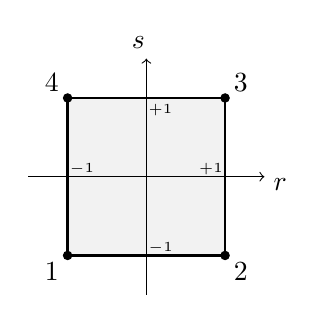
\begin{tikzpicture}
%\draw[step=0.5cm,gray,very thin] (0,0) grid (4,4); 
\draw[fill=gray!10,gray!10](1,1) rectangle (3,3);
\draw[thick] (1,1)--(3,1)--(3,3)--(1,3)--cycle;
\draw [->] (0.5,2) -- (3.5,2);
\draw [->] (2,0.5) -- (2,3.5);
\node[] at (3.7,1.9) {$r$};
\node[] at (1.9,3.7) {$s$};
\draw[black,fill=black] (1,1)   circle (1.5pt);
\draw[black,fill=black] (3,1)   circle (1.5pt);
\draw[black,fill=black] (3,3)   circle (1.5pt);
\draw[black,fill=black] (1,3)   circle (1.5pt);
\node[] at (0.8,0.8) {$1$};
\node[] at (0.8,3.2) {$4$};
\node[] at (3.2,0.8) {$2$};
\node[] at (3.2,3.2) {$3$};
\node[] at (1.18,2.1) {\tiny $-1$};
\node[] at (2.82,2.1) {\tiny $+1$};
\node[] at (2.18,1.1) {\tiny $-1$};
\node[] at (2.18,2.85) {\tiny $+1$};
\end{tikzpicture}
\end{center}



Note the counter-clockwise numbering\footnote{Note that in many of the python codes which 
are part of this project the numbering starts at 0.}.
This element is commonly called the reference element. How we go from the $(x,y)$ coordinate system 
to the $(r,s)$ once and vice versa will be dealt with later on.
The basis functions in the above reference element in the reduced 
coordinates system $(r,s)$ are given by:

\begin{mdframed}[backgroundcolor=blue!5]
\begin{eqnarray}
\bN_1(r,s)&=&0.25(1-r)(1-s) \nonumber\\
\bN_2(r,s)&=&0.25(1+r)(1-s) \nonumber\\
\bN_3(r,s)&=&0.25(1+r)(1+s) \nonumber\\
\bN_4(r,s)&=&0.25(1-r)(1+s) 
\end{eqnarray}
\end{mdframed}
These basis functions are the product of the linear basis functions of Section~\ref{sec:bf1}
in the $r$ direction and the $s$ direction.
The partial derivatives of these functions with respect to $r$ ans $s$ automatically follow:

\begin{mdframed}[backgroundcolor=blue!5]
\begin{align}
\frac{\partial \bN_1}{\partial r}(r,s)&= - 0.25(1-s) &
\frac{\partial \bN_1}{\partial s}(r,s)&= - 0.25(1-r) \nonumber\\
\frac{\partial \bN_2}{\partial r}(r,s)&= + 0.25(1-s) &
\frac{\partial \bN_2}{\partial s}(r,s)&= - 0.25(1+r) \nonumber\\
\frac{\partial \bN_3}{\partial r}(r,s)&= + 0.25(1+s) &
\frac{\partial \bN_3}{\partial s}(r,s)&= + 0.25(1+r) \nonumber\\
\frac{\partial \bN_4}{\partial r}(r,s)&= - 0.25(1+s) &
\frac{\partial \bN_4}{\partial s}(r,s)&= + 0.25(1-r) \nonumber
\end{align}
\end{mdframed}

Let us go back to Eq.~\eqref{bf01} and let us assume that the 
function $v(r,s)=C$ so that $v_i=C$ for $i=1,2,3,4$. 
It then follows that 
\[
v^h(r,s) = \sum_{i=1}^4 \bN_i(r,s)\;  v_i 
=C \sum_{i=1}^4 \bN_i(r,s)
=C [
\bN_1(r,s)
+\bN_2(r,s)
+\bN_3(r,s)
+\bN_4(r,s)]=C
\]
This is a very important property: if the $v$ function used to 
assign values at the vertices is constant, then 
the value of $v^h$ {\it anywhere} in the element is exactly $C$.
If we now turn to the derivatives of $v$ with respect to $r$ and $s$:
\[
\frac{\partial {v}^h}{\partial r}(r,s) 
= \sum_{i=1}^4 \frac{\partial \bN_i}{\partial r}(r,s)\;  v_i 
= C \sum_{i=1}^4 \frac{\partial \bN_i}{\partial r}(r,s) 
= C \left[ - 0.25(1-s)  + 0.25(1-s)  + 0.25(1+s)  - 0.25(1+s) \right] = 0 
\]

\[
\frac{\partial v^h}{\partial s}(r,s) 
= \sum_{i=1}^4 \frac{\partial \bN_i}{\partial s}(r,s)\;  v_i 
= C \sum_{i=1}^4 \frac{\partial \bN_i}{\partial s}(r,s) 
= C \left[ - 0.25(1-r) - 0.25(1+r) + 0.25(1+r) + 0.25(1-r) \right] = 0 
\]
We reassuringly find that the derivative of a constant field anywhere in the element is exactly zero.

If we now choose $v(r,s)=ar+bs$ with $a$ and $b$ two constant scalars, we find:
\begin{eqnarray}
v^h(r,s) 
&=& \sum_{i=1}^4 \bN_i(r,s)\;  v_i  \nn\\
&=& \sum_{i=1}^4 \bN_i(r,s) (ar_i+bs_i) \nn\\
&=& a \sum_{i=1}^4 \bN_i(r,s) r_i + b \sum_{i=1}^4 \bN_i(r,s) s_i \nn\\
&=& a \left[ 
 \frac14(1-r)(1-s)(-1)
+\frac14(1+r)(1-s)(+1)
+\frac14(1+r)(1+s)(+1)
+\frac14(1-r)(1+s)(-1) \right]  \nonumber\\
&+& b  
\left[ 
 \frac14(1-r)(1-s)(-1)
+\frac14(1+r)(1-s)(-1)
+\frac14(1+r)(1+s)(+1)
+\frac14(1-r)(1+s)(+1) \right]  \nonumber\\
&=& \frac{a}{4} \left[ 
-(1-r)(1-s)
+(1+r)(1-s)
+(1+r)(1+s)
-(1-r)(1+s) \right]  \nonumber\\
&+& \frac{b}{4}
\left[ 
-(1-r)(1-s)
-(1+r)(1-s)
+(1+r)(1+s)
+(1-r)(1+s) 
\right]  \nonumber\\
&=& ar+bs
\end{eqnarray}
This set of bilinear basis functions is therefore capable of exactly representing a bilinear field.
The derivatives are:
\begin{eqnarray}
\frac{\partial v^h}{\partial r}(r,s) 
&=& \sum_{i=1}^4 \frac{\partial \bN_i}{\partial r}(r,s)\;  v_i  \\
&=& a \sum_{i=1}^4 \frac{\partial \bN_i}{\partial r}(r,s) r_i 
+ b \sum_{i=1}^4 \frac{\partial \bN_i}{\partial r}(r,s) s_i \\
&=& a \left[
- \frac14(1-s)(-1) 
+ \frac14(1-s)(+1) 
+ \frac14(1+s)(+1) 
- \frac14(1+s)(-1) 
\right] \nonumber\\
&+&b \left[
- \frac14(1-s)(-1) 
+ \frac14(1-s)(-1) 
+ \frac14(1+s)(+1) 
- \frac14(1+s)(+1) 
\right] \nonumber\\
&=& \frac{a}{4} \left[
 (1-s)
+ (1-s)
+ (1+s)
+ (1+s)
\right] \nonumber\\
&+&\frac{b}{4} \left[
 (1-s)
- (1-s)
+ (1+s)
- (1+s)
\right] \nonumber\\
&=& a 
\end{eqnarray}
Here again, we find that the derivative of the bilinear field inside the element is exact: 
$\frac{\partial v^h}{\partial r} = \frac{\partial v}{\partial r}$.

However, following the same methodology as above, one can easily prove 
that this is no more true for polynomials of degree strictly higher than 1. 
This fact has serious consequences: if the solution to the problem at hand is 
for instance a parabola, the $Q_1$ basis functions cannot represent the solution properly, 
but only by approximating the parabola in each element by a line. As we will see 
later, $Q_2$ basis functions can remedy this problem by containing quadratic terms.

\begin{remark}
The $Q_1$ basis functions are first-order polynomials. We have seen that they can be used to compute
gradients. However they cannot be used to compute 2nd-order derivatives since their 2nd-order
derivative is identically zero.
\end{remark}




%%%%%%%%%%%%%%%%%%%%%%%%%%%%%%%%%%%%%%%%%%%%%%%%%%%%%%%%%%%%%%%%%%%%%%%%%%%%%%
\subsubsection{Biquadratic basis functions in 2D ($Q_2$)}\label{ss:q22d}
\index{general}{$Q_2$}

\begin{flushright} {\tiny {\color{gray} basis\_Q2\_2D.tex}} \end{flushright}
%~~~~~~~~~~~~~~~~~~~~~~~~~~~~~~~~~~~~~~~~~~~~~~~~~~~~~~~~~~~~~~~~~~~~~~~~~~~~~~~~~~~~~~~~~~~~~~~~~~

This element is part of the so-called Lagrange family \cite{raki00}. 
Inside an element the local numbering of the nodes is as follows\footnote{I have adopted here 
a numbering scheme starting at zero!}:

\begin{flushright} {\tiny {\color{gray} (tikz\_q22d.tex)}} \end{flushright}
%~~~~~~~~~~~~~~~~~~~~~~~~~~~~~~~~~~~~~~~~~~~~~~~~~~~~~~~~~~~~~~~~~~~~~~~~~~~~~~~~~~~~~~~~~~~~~~~~~~

\begin{center}
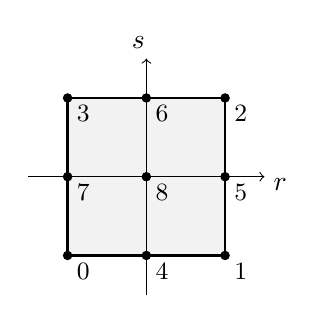
\begin{tikzpicture}
%\draw[step=0.5cm,gray,very thin] (0,0) grid (4,4); 
\draw[fill=gray!10,gray!10](1,1) rectangle (3,3);
\draw[thick] (1,1)--(3,1)--(3,3)--(1,3)--cycle;
\draw [->] (0.5,2) -- (3.5,2);
\draw [->] (2,0.5) -- (2,3.5);
\node[] at (3.7,1.9) {$r$};
\node[] at (1.9,3.7) {$s$};
\draw[black,fill=black] (1,1)   circle (1.5pt);
\draw[black,fill=black] (1,2)   circle (1.5pt);
\draw[black,fill=black] (1,3)   circle (1.5pt);
\draw[black,fill=black] (2,1)   circle (1.5pt);
\draw[black,fill=black] (2,2)   circle (1.5pt);
\draw[black,fill=black] (2,3)   circle (1.5pt);
\draw[black,fill=black] (3,1)   circle (1.5pt);
\draw[black,fill=black] (3,2)   circle (1.5pt);
\draw[black,fill=black] (3,3)   circle (1.5pt);
\node[] at (1.2,0.8) {\small $0$};
\node[] at (2.2,0.8) {\small $4$};
\node[] at (3.2,0.8) {\small $1$};
\node[] at (1.2,1.8) {\small $7$};
\node[] at (2.2,1.8) {\small $8$};
\node[] at (3.2,1.8) {\small $5$};
\node[] at (1.2,2.8) {\small $3$};
\node[] at (2.2,2.8) {\small $6$};
\node[] at (3.2,2.8) {\small $2$};
\end{tikzpicture}
\end{center}



Note that this numbering is also employed in Li \cite[p56]{li06}.
The polynomial representation of the function $\phi$ over this element is then
\[
\phi^h(r,s) = a + br + cs + drs + er^2 + fs^2 + gr^2s + hrs^2 + i r^2s^2 = \sum_{i=0}^8 \bN_i(r,s) \phi_i
\]
and one can show that the basis functions are:
\begin{mdframed}[backgroundcolor=blue!5]
\begin{eqnarray}
\bN_0(r,s)&=& \frac{1}{2}r(r-1)  \frac{1}{2}s(s-1)\nonumber\\
\bN_1(r,s)&=& \frac{1}{2}r(r+1)  \frac{1}{2}s(s-1)\nonumber\\
\bN_2(r,s)&=& \frac{1}{2}r(r+1)  \frac{1}{2}s(s+1)\nonumber\\
\bN_3(r,s)&=& \frac{1}{2}r(r-1)  \frac{1}{2}s(s+1)\nonumber\\
\bN_4(r,s)&=&     (1-r^2)  \frac{1}{2}s(s-1)\nonumber\\
\bN_5(r,s)&=& \frac{1}{2}r(r+1)      (1-s^2)\nonumber\\
\bN_6(r,s)&=&     (1-r^2)  \frac{1}{2}s(s+1)\nonumber\\
\bN_7(r,s)&=& \frac{1}{2}r(r-1)      (1-s^2)\nonumber\\
\bN_8(r,s)&=&     (1-r^2)      (1-s^2)\nonumber
\end{eqnarray}
\end{mdframed}

Note that we have $\bN_i(r_j,s_j)=\delta_{ij}$ and $\bN_i(r_i,s_i)=1$. 

Their derivatives are given by:
\begin{mdframed}[backgroundcolor=blue!5]
\begin{align}
\frac{\partial \bN_0}{\partial r}&= \frac{1}{2}(2r-1)  \frac{1}{2}s(s-1) & 
\frac{\partial \bN_0}{\partial s}&= \frac{1}{2}r(r-1)  \frac{1}{2}(2s-1)\nonumber\\
\frac{\partial \bN_1}{\partial r}&= \frac{1}{2}(2r+1)  \frac{1}{2}s(s-1) &
\frac{\partial \bN_1}{\partial s}&= \frac{1}{2}r(r+1)  \frac{1}{2}(2s-1)\nonumber\\
\frac{\partial \bN_2}{\partial r}&= \frac{1}{2}(2r+1)  \frac{1}{2}s(s+1) &
\frac{\partial \bN_2}{\partial s}&= \frac{1}{2}r(r+1)  \frac{1}{2}(2s+1)\nonumber\\
\frac{\partial \bN_3}{\partial r}&= \frac{1}{2}(2r-1)  \frac{1}{2}s(s+1) &
\frac{\partial \bN_3}{\partial s}&= \frac{1}{2}r(r-1)  \frac{1}{2}(2s+1)\nonumber\\
\frac{\partial \bN_4}{\partial r}&=       (-2r)  \frac{1}{2}s(s-1) &
\frac{\partial \bN_4}{\partial s}&=     (1-r^2)  \frac{1}{2}(2s-1)\nonumber\\
\frac{\partial \bN_5}{\partial r}&= \frac{1}{2}(2r+1)     (1-s^2)&
\frac{\partial \bN_5}{\partial s}&= \frac{1}{2}r(r+1)        (-2s)\nonumber\\
\frac{\partial \bN_6}{\partial r}&=       (-2r)  \frac{1}{2}s(s+1)&
\frac{\partial \bN_6}{\partial s}&=     (1-r^2)  \frac{1}{2}(2s+1)\nonumber\\
\frac{\partial \bN_7}{\partial r}&= \frac{1}{2}(2r-1)     (1-s^2)&
\frac{\partial \bN_7}{\partial s}&= \frac{1}{2}r(r-1)        (-2s)\nonumber\\
\frac{\partial \bN_8}{\partial r}&=       (-2r)     (1-s^2)&
\frac{\partial \bN_8}{\partial s}&=     (1-r^2)        (-2s)\nonumber
\end{align}
\end{mdframed}


%%%%%%%%%%%%%%%%%%%%%%%%%%%%%%%%%%%%%%%%%%%%%%%%%%%%%%%%%%%%%%%%%%%%%%%%%%%%%%
\subsubsection{Bicubic basis functions in 2D ($Q_3$)}
\index{general}{$Q_3$}

\begin{flushright} {\tiny {\color{gray} basis\_Q3\_2D.tex}} \end{flushright}
%~~~~~~~~~~~~~~~~~~~~~~~~~~~~~~~~~~~~~~~~~~~~~~~~~~~~~~~~~~~~~~~~~~~~~~~~~~~~~~~~~~~~~~~~~~~~~~~~~~

Inside an element the local numbering of the nodes is as follows:

\begin{flushright} {\tiny {\color{gray} (tikz\_q32d.tex)}} \end{flushright}
%~~~~~~~~~~~~~~~~~~~~~~~~~~~~~~~~~~~~~~~~~~~~~~~~~~~~~~~~~~~~~~~~~~~~~~~~~~~~~~~~~~~~~~~~~~~~~~~~~~


\begin{center}
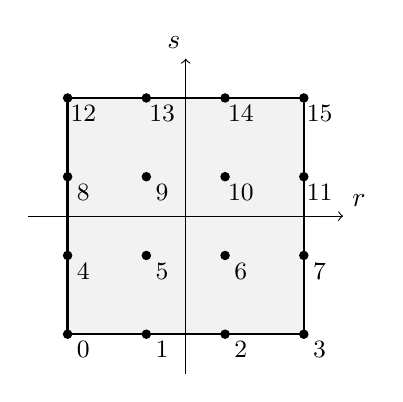
\begin{tikzpicture}
%\draw[step=0.5cm,gray,very thin] (0,0) grid (5,5); 
\draw[fill=gray!10,gray!10](1,1) rectangle (4,4);
\draw[thick] (1,1)--(4,1)--(4,4)--(1,4)--cycle;
\draw [->] (0.5,2.5) -- (4.5,2.5);
\draw [->] (2.5,0.5) -- (2.5,4.5);
\node[] at (4.7,2.7) {$r$};
\node[] at (2.35,4.7) {$s$};
\draw[black,fill=black] (1,1)   circle (1.5pt);
\draw[black,fill=black] (1,2)   circle (1.5pt);
\draw[black,fill=black] (1,3)   circle (1.5pt);
\draw[black,fill=black] (1,4)   circle (1.5pt);
\draw[black,fill=black] (2,1)   circle (1.5pt);
\draw[black,fill=black] (2,2)   circle (1.5pt);
\draw[black,fill=black] (2,3)   circle (1.5pt);
\draw[black,fill=black] (2,4)   circle (1.5pt);
\draw[black,fill=black] (3,1)   circle (1.5pt);
\draw[black,fill=black] (3,2)   circle (1.5pt);
\draw[black,fill=black] (3,3)   circle (1.5pt);
\draw[black,fill=black] (3,4)   circle (1.5pt);
\draw[black,fill=black] (4,1)   circle (1.5pt);
\draw[black,fill=black] (4,2)   circle (1.5pt);
\draw[black,fill=black] (4,3)   circle (1.5pt);
\draw[black,fill=black] (4,4)   circle (1.5pt);
\node[] at (1.2,0.8) {\small $0$};
\node[] at (2.2,0.8) {\small $1$};
\node[] at (3.2,0.8) {\small $2$};
\node[] at (4.2,0.8) {\small $3$};
\node[] at (1.2,1.8) {\small $4$};
\node[] at (2.2,1.8) {\small $5$};
\node[] at (3.2,1.8) {\small $6$};
\node[] at (4.2,1.8) {\small $7$};
\node[] at (1.2,2.8) {\small $8$};
\node[] at (2.2,2.8) {\small $9$};
\node[] at (3.2,2.8) {\small $10$};
\node[] at (4.2,2.8) {\small $11$};
\node[] at (1.2,3.8) {\small $12$};
\node[] at (2.2,3.8) {\small $13$};
\node[] at (3.2,3.8) {\small $14$};
\node[] at (4.2,3.8) {\small $15$};
\end{tikzpicture}
\end{center}



The 1D cubic basis functions are given by:
\begin{align}
\bN_1(r)&=(-1   +r +9r^2 - 9r^3)/16 & \bN_1(t)&=(-1   +t +9t^2 - 9t^3)/16 \nonumber\\
\bN_2(r)&=(+9 -27r -9r^2 +27r^3)/16 & \bN_2(t)&=(+9 -27t -9t^2 +27t^3)/16 \nonumber\\
\bN_3(r)&=(+9 +27r -9r^2 -27r^3)/16 & \bN_3(t)&=(+9 +27t -9t^2 -27t^3)/16 \nonumber\\
\bN_4(r)&=(-1   -r +9r^2 + 9r^3)/16 & \bN_4(t)&=(-1   -t +9t^2 + 9t^3)/16 \nonumber
\end{align}

The resulting basis functions are simply the tensor product of the above 1D ones:

\begin{mdframed}[backgroundcolor=blue!5]
\begin{eqnarray}
\bN_{01}(r,s)&=&\bN_1(r)\bN_1(s) = (-1   +r +9r^2 - 9r^3)/16 \cdot (-1  +t +9s^2 - 9s^3)/16 \nonumber\\
\bN_{02}(r,s)&=&\bN_2(r)\bN_1(s) = (+9 -27r -9r^2 +27r^3)/16 \cdot (-1  +t +9s^2 - 9s^3)/16 \nonumber\\
\bN_{03}(r,s)&=&\bN_3(r)\bN_1(s) = (+9 +27r -9r^2 -27r^3)/16 \cdot (-1  +t +9s^2 - 9s^3)/16 \nonumber\\
\bN_{04}(r,s)&=&\bN_4(r)\bN_1(s) = (-1   -r +9r^2 + 9r^3)/16 \cdot (-1  +t +9s^2 - 9s^3)/16 \nonumber\\
\bN_{05}(r,s)&=&\bN_1(r)\bN_2(s) = (-1   +r +9r^2 - 9r^3)/16 \cdot (9 -27s -9s^2 +27s^3)/16 \nonumber\\
\bN_{06}(r,s)&=&\bN_2(r)\bN_2(s) = (+9 -27r -9r^2 +27r^3)/16 \cdot (9 -27s -9s^2 +27s^3)/16 \nonumber\\
\bN_{07}(r,s)&=&\bN_3(r)\bN_2(s) = (+9 +27r -9r^2 -27r^3)/16 \cdot (9 -27s -9s^2 +27s^3)/16 \nonumber\\
\bN_{08}(r,s)&=&\bN_4(r)\bN_2(s) = (-1   -r +9r^2 + 9r^3)/16 \cdot (9 -27s -9s^2 +27s^3)/16 \nonumber\\
\bN_{09}(r,s)&=&\bN_1(r)\bN_3(s) = (-1   +r +9r^2 - 9r^3)/16 \cdot (9 +27t -9t^2 -27t^3)/16 \nn\\
\bN_{10}(r,s)&=&\bN_2(r)\bN_3(s) = (+9 -27r -9r^2 +27r^3)/16 \cdot (9 +27t -9t^2 -27t^3)/16 \nn\\
\bN_{11}(r,s)&=&\bN_3(r)\bN_3(s) = (+9 +27r -9r^2 -27r^3)/16 \cdot (9 +27t -9t^2 -27t^3)/16 \nn\\
\bN_{12}(r,s)&=&\bN_4(r)\bN_3(s) = (-1   -r +9r^2 + 9r^3)/16 \cdot (9 +27t -9t^2 -27t^3)/16 \nn\\
\bN_{13}(r,s)&=&\bN_1(r)\bN_4(s) = (-1   +r +9r^2 - 9r^3)/16 \cdot (-1   -t +9t^2 + 9t^3)/16\nn\\
\bN_{14}(r,s)&=&\bN_2(r)\bN_4(s) = (+9 -27r -9r^2 +27r^3)/16 \cdot (-1   -t +9t^2 + 9t^3)/16\nn\\
\bN_{15}(r,s)&=&\bN_3(r)\bN_4(s) = (+9 +27r -9r^2 -27r^3)/16 \cdot (-1   -t +9t^2 + 9t^3)/16\nn\\
\bN_{16}(r,s)&=&\bN_4(r)\bN_4(s) = (-1   -r +9r^2 + 9r^3)/16 \cdot (-1   -t +9t^2 + 9t^3)/16
\end{eqnarray}
\end{mdframed}

\begin{center}
\includegraphics[width=4cm]{images/basis_Q3_2D/N1}
\includegraphics[width=4cm]{images/basis_Q3_2D/N2}
\includegraphics[width=4cm]{images/basis_Q3_2D/N3}
\includegraphics[width=4cm]{images/basis_Q3_2D/N4}\\
\includegraphics[width=4cm]{images/basis_Q3_2D/N5}
\includegraphics[width=4cm]{images/basis_Q3_2D/N6}
\includegraphics[width=4cm]{images/basis_Q3_2D/N7}
\includegraphics[width=4cm]{images/basis_Q3_2D/N8}\\
\includegraphics[width=4cm]{images/basis_Q3_2D/N9}
\includegraphics[width=4cm]{images/basis_Q3_2D/N10}
\includegraphics[width=4cm]{images/basis_Q3_2D/N11}
\includegraphics[width=4cm]{images/basis_Q3_2D/N12}\\
\includegraphics[width=4cm]{images/basis_Q3_2D/N13}
\includegraphics[width=4cm]{images/basis_Q3_2D/N14}
\includegraphics[width=4cm]{images/basis_Q3_2D/N15}
\includegraphics[width=4cm]{images/basis_Q3_2D/N16}\\
{\captionfont Surface representation of the basis functions on the reference element.\\
{\color{gray} in images/basis\_Q3\_2D/ }}
\end{center}

The derivatives are trivial to obtain from the derivatives of the 1D basis functions, 
e.g.
\[
\frac{\partial \bN_{13}}{\partial r} = 
\frac{\partial \bN_{1}}{\partial r} \bN_4(s) 
\]

These basis functions are used in \stone 19.










%%%%%%%%%%%%%%%%%%%%%%%%%%%%%%%%%%%%%%%%%%%%%%%%%%%%%%%%%%%%%%%%%%%%%
\subsubsection{Eight node serendipity basis functions in 2D ($Q_2^{(8)}$)}
\label{sec:serendipity2D}
\index{general}{$Q_2^{(8)}$} 
\index{general}{Serendipity element}

\begin{flushright} {\tiny {\color{gray} basis\_Q28\_2D.tex}} \end{flushright}
%~~~~~~~~~~~~~~~~~~~~~~~~~~~~~~~~~~~~~~~~~~~~~~~~~~~~~~~~~~~~~~~~~~~~~~~~~~~~~~~~~~~~~~~~~~~~~~~~~~

The serendipity elements are those rectangular elements which have no
interior nodes (See for example Reddy \cite[p65]{reddybook2}).
Inside an element a possible local numbering of the nodes is as follows:

\input{tikz/tikz_serendipity2D}

The main difference with the $Q_2$ element resides in the fact that there is 
no node in the middle of the element.
The polynomial representation of the function $\phi$ over the element is then
\[
\phi_h(r,s) = a + br + cs + drs + er^2 + fs^2 + gr^2s + hrs^2
\]
Note that absence of the $r^2s^2$ term which was previously associated 
to the center node. We find that 
\begin{mdframed}[backgroundcolor=blue!5]
\begin{eqnarray}
\bN_0(r,s)&=& \frac{1}{4}(1-r)(1-s)(-r-s-1) \\
\bN_1(r,s)&=& \frac{1}{4}(1+r)(1-s)(r-s-1) \\
\bN_2(r,s)&=& \frac{1}{4}(1+r)(1+s)(r+s-1) \\
\bN_3(r,s)&=& \frac{1}{4}(1-r)(1+s)(-r+s-1) \\
\bN_4(r,s)&=& \frac{1}{2}(1-r^2)(1-s)  \\
\bN_5(r,s)&=& \frac{1}{2}(1+r)  (1-s^2)\\
\bN_6(r,s)&=& \frac{1}{2}(1-r^2)(1+s)  \\
\bN_7(r,s)&=& \frac{1}{2}(1-r)  (1-s^2)
\end{eqnarray}
\end{mdframed}

The basis functions at the mid side nodes are products of a 
second order polynomial parallel to side and 
a linear function perpendicular to the side
while basis functions for corner nodes are modifications of the bilinear
quadrilateral element.

\begin{center}
\includegraphics[width=4cm]{images/basis_Q28_2D/N1}
\includegraphics[width=4cm]{images/basis_Q28_2D/N2}
\includegraphics[width=4cm]{images/basis_Q28_2D/N3}
\includegraphics[width=4cm]{images/basis_Q28_2D/N4}\\
\includegraphics[width=4cm]{images/basis_Q28_2D/N5}
\includegraphics[width=4cm]{images/basis_Q28_2D/N6}
\includegraphics[width=4cm]{images/basis_Q28_2D/N7}
\includegraphics[width=4cm]{images/basis_Q28_2D/N8}\\
{\captionfont Surface representation of the basis functions on the reference element.
{\color{gray} in images/basis\_Q28\_2D/ }}
\end{center}



The first-order derivatives are given by:

\begin{mdframed}[backgroundcolor=blue!5]
\begin{eqnarray}
\frac{\partial \bN_0}{\partial r}(r,s)&=& -\frac{1}{4}(s-1)(2r+s)  \\
\frac{\partial \bN_1}{\partial r}(r,s)&=& -\frac{1}{4}(s-1)(2r-s)  \\
\frac{\partial \bN_2}{\partial r}(r,s)&=& \frac{1}{4}(s+1)(2r+s)  \\
\frac{\partial \bN_3}{\partial r}(r,s)&=& \frac{1}{4}(s+1)(2r-s)  \\
\frac{\partial \bN_4}{\partial r}(r,s)&=& r(s-1)  \\
\frac{\partial \bN_5}{\partial r}(r,s)&=& \frac{1}{2} (1-s^2)  \\
\frac{\partial \bN_6}{\partial r}(r,s)&=& -r(s+1)  \\
\frac{\partial \bN_7}{\partial r}(r,s)&=& -\frac{1}{2} (1-s^2)  
\end{eqnarray}
\end{mdframed}

\begin{mdframed}[backgroundcolor=blue!5]
\begin{eqnarray}
\frac{\partial \bN_0}{\partial s}(r,s)&=& -\frac{1}{4}(r-1)(r+2s) \\
\frac{\partial \bN_1}{\partial s}(r,s)&=& -\frac{1}{4}(r+1)(r-2s) \\
\frac{\partial \bN_2}{\partial s}(r,s)&=&  \frac{1}{4}(r+1)(r+2s) \\
\frac{\partial \bN_3}{\partial s}(r,s)&=&  \frac{1}{4}(r-1)(r-2s) \\
\frac{\partial \bN_4}{\partial s}(r,s)&=& - \frac{1}{2}(1-r^2)\\
\frac{\partial \bN_5}{\partial s}(r,s)&=&  -(r+1)s \\
\frac{\partial \bN_6}{\partial s}(r,s)&=& \frac{1}{2} (1-r^2)\\
\frac{\partial \bN_7}{\partial s}(r,s)&=&  (r-1)s
\end{eqnarray}
\end{mdframed}
These basis functions are used in \stone 52.













%%%%%%%%%%%%%%%%%%%%%%%%%%%%%%%%%%%%%%%%%%%%%%%%%%%%%%%%%%%%%%%%%%%%%
\subsubsection{Eight node serendipity basis functions in 2D ($QH8-C1$)}
\label{sec:serendipity2Db}
\index{general}{$QH8-C1$} \index{general}{Serendipity element}

This element is proposed in Zhang \& Xiang (2020) \cite{zhxi20}. Two remarks
must be made: 1) Eq.~(29) of their publication which is the definition
of the basis functions contains an error\footnote{
Answer from the author: "N5 to N8 is missing an A in the denominator and 
the calculation program does not have this problem"}. 2) The authors use a rather 
uncommon and annoying rotated numbering:
\begin{verbatim}
      y
      |
2=====5=====1             3=====6=====2
|           |             |           |   (r_0,s_0)=(-1,-1)   (r_4,s_4)=( 0,-1)
|           |             |           |   (r_1,s_1)=(+1,-1)   (r_5,s_5)=(+1, 0)
6           8--x          7     +     5   (r_2,s_2)=(+1,+1)   (r_6,s_6)=( 0,+1)
|           |             |           |   (r_3,s_3)=(-1,+1)   (r_7,s_7)=(-1, 0)
|           |             |           |    
3=====7=====4             0=====4=====1
Zhang & Xiang             our numbering
\end{verbatim}

For each element they define (their numbering):
\begin{eqnarray}
A   &=& \frac{1}{2} [ (x_1-x_3)(y_2-y_4)-(x_2-x_4)(y_1-y_3) ] \nn\\
m_x &=& (x_1-x_4)(y_2-y_3)-(x_2-x_3)(y_1-y_4) \nn\\
m_y &=& (x_3-x_4)(y_1-y_2)-(x_1-x_2)(y_3-y_4) \nn
\end{eqnarray}

Note that $A$ is the area of the element, and that in the case when 
the element is a rectangle then $m_x=m_y=0$.

\begin{eqnarray}
\bN_1(r,s)&=& n_1(r,s) +(m_x^2 - m_xm_y + m_y^2)\frac{E(r,s)}{D} \nn\\
\bN_2(r,s)&=& n_2(r,s) +(m_x^2 + m_xm_y + m_y^2)\frac{E(r,s)}{D} \nn\\
\bN_3(r,s)&=& n_3(r,s) +(m_x^2 - m_xm_y + m_y^2)\frac{E(r,s)}{D} \nn\\
\bN_4(r,s)&=& n_4(r,s) +(m_x^2 + m_xm_y + m_y^2)\frac{E(r,s)}{D} \nn\\
\bN_5(r,s)&=& n_5(r,s) -m_x(2Am_x+m_y^2)\frac{E(r,s)}{AD} \nn\\
\bN_6(r,s)&=& n_6(r,s) -m_y(2Am_y+m_x^2)\frac{E(r,s)}{AD} \nn\\
\bN_7(r,s)&=& n_7(r,s) +m_x(-2Am_x+m_y^2)\frac{E(r,s)}{AD} \nn\\
\bN_8(r,s)&=& n_8(r,s) +m_y(-2Am_y+m_x^2)\frac{E(r,s)}{AD} \nn
\end{eqnarray}
with 
\[
E(r,s)=(1-r^2)(1-s^2)
\qquad
D=4(4A^2+m_x^2+m_y^2)
\]
and where the $n_i$ functions are the basis functions of the 'regular' 
8-node element (see Section~\ref{sec:serendipity2D}).

This is implemented in \stone 52.

\todo[inline]{not finished. SHOW CONSISTENCY !! like in paper
email sent to author about mistake.  }








%%%%%%%%%%%%%%%%%%%%%%%%%%%%%%%%%%%%
\subsubsection{Biquartic basis functions in 2D ($Q_4$)}
\index{general}{$Q_4$}

Inside an element the local numbering of the nodes is as follows:

\begin{flushright} {\tiny {\color{gray} (tikz\_q42d.tex)}} \end{flushright}
%~~~~~~~~~~~~~~~~~~~~~~~~~~~~~~~~~~~~~~~~~~~~~~~~~~~~~~~~~~~~~~~~~~~~~~~~~~~~~~~~~~~~~~~~~~~~~~~~~~


\begin{center}
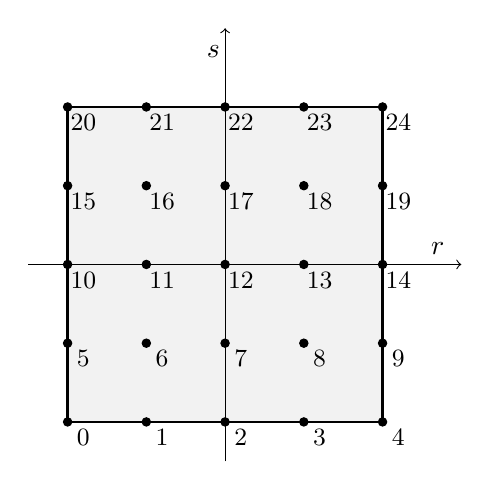
\begin{tikzpicture}
%\draw[step=0.5cm,gray,very thin] (0,0) grid (5,5); 
\draw[fill=gray!10,gray!10](1,1) rectangle (5,5);
\draw[thick] (1,1)--(5,1)--(5,5)--(1,5)--cycle;
\draw [->] (0.5,3) -- (6,3);
\draw [->] (3,0.5) -- (3,6);
\node[] at (5.7,3.2) {$r$};
\node[] at (2.85,5.7) {$s$};
\draw[black,fill=black] (1,1)   circle (1.5pt);
\draw[black,fill=black] (1,2)   circle (1.5pt);
\draw[black,fill=black] (1,3)   circle (1.5pt);
\draw[black,fill=black] (1,4)   circle (1.5pt);
\draw[black,fill=black] (1,5)   circle (1.5pt);

\draw[black,fill=black] (2,1)   circle (1.5pt);
\draw[black,fill=black] (2,2)   circle (1.5pt);
\draw[black,fill=black] (2,3)   circle (1.5pt);
\draw[black,fill=black] (2,4)   circle (1.5pt);
\draw[black,fill=black] (2,5)   circle (1.5pt);

\draw[black,fill=black] (3,1)   circle (1.5pt);
\draw[black,fill=black] (3,2)   circle (1.5pt);
\draw[black,fill=black] (3,3)   circle (1.5pt);
\draw[black,fill=black] (3,4)   circle (1.5pt);
\draw[black,fill=black] (3,5)   circle (1.5pt);

\draw[black,fill=black] (4,1)   circle (1.5pt);
\draw[black,fill=black] (4,2)   circle (1.5pt);
\draw[black,fill=black] (4,3)   circle (1.5pt);
\draw[black,fill=black] (4,4)   circle (1.5pt);
\draw[black,fill=black] (4,5)   circle (1.5pt);

\draw[black,fill=black] (5,1)   circle (1.5pt);
\draw[black,fill=black] (5,2)   circle (1.5pt);
\draw[black,fill=black] (5,3)   circle (1.5pt);
\draw[black,fill=black] (5,4)   circle (1.5pt);
\draw[black,fill=black] (5,5)   circle (1.5pt);

\node[] at (1.2,0.8) {\small $0$};
\node[] at (2.2,0.8) {\small $1$};
\node[] at (3.2,0.8) {\small $2$};
\node[] at (4.2,0.8) {\small $3$};
\node[] at (5.2,0.8) {\small $4$};

\node[] at (1.2,1.8) {\small $5$};
\node[] at (2.2,1.8) {\small $6$};
\node[] at (3.2,1.8) {\small $7$};
\node[] at (4.2,1.8) {\small $8$};
\node[] at (5.2,1.8) {\small $9$};

\node[] at (1.2,2.8) {\small $10$};
\node[] at (2.2,2.8) {\small $11$};
\node[] at (3.2,2.8) {\small $12$};
\node[] at (4.2,2.8) {\small $13$};
\node[] at (5.2,2.8) {\small $14$};

\node[] at (1.2,3.8) {\small $15$};
\node[] at (2.2,3.8) {\small $16$};
\node[] at (3.2,3.8) {\small $17$};
\node[] at (4.2,3.8) {\small $18$};
\node[] at (5.2,3.8) {\small $19$};

\node[] at (1.2,4.8) {\small $20$};
\node[] at (2.2,4.8) {\small $21$};
\node[] at (3.2,4.8) {\small $22$};
\node[] at (4.2,4.8) {\small $23$};
\node[] at (5.2,4.8) {\small $24$};

\end{tikzpicture}
\end{center}



%.....................................................................
\subsubsection{Linear basis functions for triangles in 2D ($P_1$)}\label{ss:p1}
\index{general}{$P_1$}

\begin{flushright} {\tiny {\color{gray} basis\_P1\_2D.tex}} \end{flushright}
%~~~~~~~~~~~~~~~~~~~~~~~~~~~~~~~~~~~~~~~~~~~~~~~~~~~~~~~~~~~~~~~~~~~~~~~~~~~~~~~~~~~~~~~~~~~~~~~~~~

Here we do not start from a reference element but consider instead a generic triangle:

\begin{flushright} {\tiny {\color{gray} (tikz\_P1.tex)}} \end{flushright}
%~~~~~~~~~~~~~~~~~~~~~~~~~~~~~~~~~~~~~~~~~~~~~~~~~~~~~~~~~~~~~~~~~~~~~~~~~~~~~~~~~~~~~~~~~~~~~~~~~~

\begin{center}
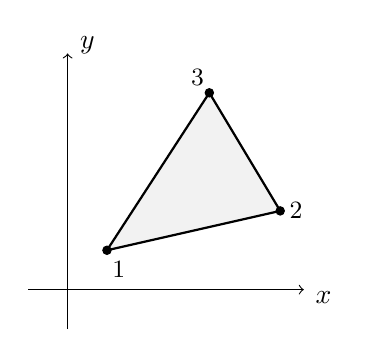
\begin{tikzpicture}
%\draw[step=0.5cm,gray,very thin] (0,0) grid (4,4); 
\draw[fill=gray!10,gray!10](1,1) (1,1)--(3.2,1.5)--(2.3,3)--cycle;
\draw[thick] (1,1)--(3.2,1.5)--(2.3,3)--cycle;
\draw [->] (0,0.5) -- (3.5,0.5);
\draw [->] (0.5,0) -- (0.5,3.5);
\node[] at (3.75,0.4) {$x$};
\node[] at (0.75,3.6) {$y$};
\draw[black,fill=black] (1,1)   circle (1.5pt);
\draw[black,fill=black] (3.2,1.5)   circle (1.5pt);
\draw[black,fill=black] (2.3,3)   circle (1.5pt);
\node[] at (1.15,0.75) {\small $1$};
\node[] at (3.4,1.5) {\small $2$};
\node[] at (2.15,3.2) {\small $3$};
\end{tikzpicture}
\end{center}




This is the simplest 2D element, which is also called linear triangular element.
Velocities (or displacements) $(u^h,v^h)$ in the element are interpolated from nodal velocities
$(u_i,v_i)$ using basis functions $\bN_i$ as follows,
\begin{small}
\[
\vec\upnu^h=
\left(
\begin{array}{c}
u^h(x,y) \\v^h(x,y)
\end{array}
\right)
=
\left(
\begin{array}{c}
\sum\limits_{i=1}^3 \bN_i(x,y) u_i \\
\sum\limits_{i=1}^3 \bN_i(x,y) v_i
\end{array}
\right)
=
\left(
\begin{array}{cccccc}
\bN_1(x,y) & 0 & \bN_2(x,y) & 0 & \bN_3(x,y) & 0\\
0 & \bN_1(x,y) & 0 & \bN_2(x,y) & 0 & \bN_3(x,y)\\
\end{array}
\right)
\cdot
\left(
\begin{array}{c}
u_1 \\ v_1 \\ u_2 \\ v_2 \\ u_3 \\ v_3
\end{array}
\right)
\]
\end{small}

For this element, we have three nodes at the vertices of the triangle, which are 
numbered around the element in the counterclockwise direction. 
Each node has two degrees of freedom (i.e. it can move in the $x$ and $y$ directions). 
The velocities $u^h$ and $v^h$ are assumed to be linear functions within the element, that is, 
\begin{eqnarray}
u^h(x,y)&=&b_1 +b_2x+b_3y \nn\\
v^h(x,y)&=&b_4 +b_5x+b_6y
\end{eqnarray}
where $b_i$ are constants to be determined and which depend on the triangle shape.
Note that the strain rate components are then given by
\begin{eqnarray}
\dot\varepsilon_{xx}(\vec\upnu)&=&b_2  \nn\\
\dot\varepsilon_{yy}(\vec\upnu)&=&b_6  \nn\\
\dot\varepsilon_{xy}(\vec\upnu)&=&(b_3+b_5)/2 \nn
\end{eqnarray}
and are constant throughout the element.

The velocities should satisfy the following six equations (when it is evaluated at a node we should 
recover the nodal velocity):
\begin{eqnarray}
u_1 &=& u^h(x_1,y_1)= b_1 + b_2x_1+b_3y_1 \nn\\
u_2 &=& u^h(x_2,y_2)= b_1 + b_2x_2+b_3y_2 \nn\\
u_3 &=& u^h(x_3,y_3)= b_1 + b_2x_3+b_3y_3 \nn\\
v_1 &=& v^h(x_1,y_1)= b_4 + b_5x_1+b_6y_1 \nn\\
v_2 &=& v^h(x_2,y_2)= b_4 + b_5x_2+b_6y_2 \nn\\
v_3 &=& v^h(x_3,y_3)= b_4 + b_5x_3+b_6y_3 \nn
\end{eqnarray}
Let us focus on the three equations with the $u$ component of the velocity.
These can be re-written:
\[
\left(
\begin{array}{c}
u_1 \\ u_2 \\ u_3  
\end{array}
\right)
=
\left(
\begin{array}{ccc}
1 & x_1 & y_1 \\
1 & x_2 & y_2 \\
1 & x_3 & y_3 \\
\end{array}
\right)
\cdot
\left(
\begin{array}{c}
b_1 \\ b_2 \\ b_3  
\end{array}
\right)
\]
In order to obtain $b_1,b_2,b_3$ we need to solve this system, or simply to compute the
inverse of the $3\times 3$ ${\bm M}$ matrix, as explained in Appendix~\ref{sec:inv3x3}.
We define $D={\rm det}({\bm M})$ and we get
\[
\left(
\begin{array}{c}
b_1 \\ b_2 \\ b_3  
\end{array}
\right)
=
\frac{1}{D}
\tilde{\bm M}
\cdot
\left(
\begin{array}{c}
u_1 \\ u_2 \\ u_3  
\end{array}
\right)
%\qquad
%{\rm and}
%\qquad
%\left(
%\begin{array}{c}
%b_4 \\ b_5 \\ b_6  
%\end{array}
%\right)
%=
%\frac{1}{D}
%\tilde{\bm M}
%\cdot
%\left(
%\begin{array}{c}
%v_1 \\ v_2 \\ v_3  
%\end{array}
%\right)
\]
The matrix $\tilde{\bm M}$ is given by:
\[
\tilde{\bm M}
%=
%\left(
%\begin{array}{ccc}
%  x_2y_3-x_3y_2  & -(y_3-y_2) &   x_3-x_2 \\
%-(x_1y_3-x_3y_1) &   y_3-y_1  & -(x_3-x_1) \\
%  x_1y_2-x_2y_1  & -(y_2-y_1) &   x_2-x_1
%\end{array}
%\right)
=
\left(
\begin{array}{ccc}
x_2y_3-x_3y_2 & x_3y_1-x_1y_3 & x_1y_2-x_2y_1 \\
y_2-y_3 & y_3-y_1  & y_1-y_2 \\
x_3-x_2 & x_1-x_3 & x_2-x_1 
\end{array}
\right)
\]
so that 
\begin{eqnarray}
b_1 &=& \frac1D [ (x_2y_3-x_3y_2)u_1 + (x_3y_1-x_1y_3)u_2 + (x_1y_2-x_2y_1)u_3 ] \nn\\
b_2 &=& \frac1D [ (y_2-y_3)u_1 + (y_3-y_1)u_2 + (y_1-y_2)u_3 ] \nn\\
b_3 &=& \frac1D [ (x_3-x_2)u_1 + (x_1-x_3)u_2 + (x_2-x_1)u_3 ]
\end{eqnarray}
We then have
\begin{eqnarray}
u^h(x,y) 
&=& b_1 + b_2 x + b_3 y \nn\\
&=&\frac1D [(x_2y_3-x_3y_2)u_1 + (x_3y_1-x_1y_3)u_2 + (x_1y_2-x_2y_1)u_3 ] \nn\\
&+&\frac1D [(y_2-y_3)u_1 + (y_3-y_1)u_2 + (y_1-y_2)u_3]x \nn\\
&+&\frac1D [(x_3-x_2)u_1 + (x_1-x_3)u_2 + (x_2-x_1)u_3]y \nn\\
&=&\frac1D [(x_2y_3-x_3y_2) + (y_2-y_3)x + (x_3-x_2)y]u_1\nn\\ 
&+&\frac1D [(x_3y_1-x_1y_3) + (y_3-y_1) x + (x_1-x_3) y]u_2 \nn\\
&+&\frac1D [(x_1y_2-x_2y_1) + (y_1-y_2) x + (x_2-x_1) y]u_3\nn\\
&=& \bN_1(x,y) u_1 + \bN_2(x,y) u_2 + \bN_3(x,y) u_3
\end{eqnarray}
with the linear basis functions are given by:
\begin{eqnarray}
\bN_1(x,y) &=& \frac{1}{D}[(x_2y_3-x_3y_2) + (y_2-y_3)x + (x_3-x_2)y] \nn\\
\bN_2(x,y) &=& \frac{1}{D}[(x_3y_1-x_1y_3) + (y_3-y_1)x + (x_1-x_3)y] \nn\\
\bN_3(x,y) &=& \frac{1}{D}[(x_1y_2-x_2y_1) + (y_1-y_2)x + (x_2-x_1)y] \nn
\end{eqnarray}
We can then easily verify that for example
\begin{eqnarray}
\bN_2(x_1,y_1)&=& \frac{1}{D}[(x_3y_1-x_1y_3) + (y_3-y_1)x_1 + (x_1-x_3)y_1] = 0 \\
\bN_2(x_2,y_2)&=& \frac{1}{D}[(x_3y_1-x_1y_3) + (y_3-y_1)x_2 + (x_1-x_3)y_2] = 1 \\
\bN_2(x_3,y_3)&=& \frac{1}{D}[(x_3y_1-x_1y_3) + (y_3-y_1)x_3 + (x_1-x_3)y_3] = 0 
\end{eqnarray}
Note that the area $A$ of the triangle is given by:
\[
A=\frac{1}{2}D = \frac{1}{2}
\left|
\begin{array}{ccc}
1 & x_1 & y_1 \\
1 & x_2 & y_2 \\
1 & x_3 & y_3 
\end{array}
\right|
\]

\noindent If we now consider the reference element in the reduced coordinates space $(r,s)$:

\begin{flushright} {\tiny {\color{gray} (tikz\_P1ref.tex)}} \end{flushright}
%~~~~~~~~~~~~~~~~~~~~~~~~~~~~~~~~~~~~~~~~~~~~~~~~~~~~~~~~~~~~~~~~~~~~~~~~~~~~~~~~~~~~~~~~~~~~~~~~~~


\begin{center}
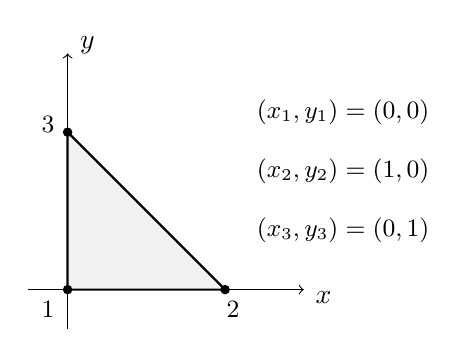
\begin{tikzpicture}
%\draw[step=0.5cm,gray,very thin] (0,0) grid (4,4); 
\draw[fill=gray!10,gray!10] (0.5,0.5)--(2.5,0.5)--(0.5,2.5)--cycle;
\draw[thick] (0.5,0.5)--(2.5,0.5)--(0.5,2.5)--cycle;
\draw [->] (0,0.5) -- (3.5,0.5);
\draw [->] (0.5,0) -- (0.5,3.5);
\node[] at (3.75,0.4) {$x$};
\node[] at (0.75,3.6) {$y$};
\draw[black,fill=black] (0.5,0.5)   circle (1.5pt);
\draw[black,fill=black] (2.5,0.5)   circle (1.5pt);
\draw[black,fill=black] (0.5,2.5)   circle (1.5pt);
\node[] at (0.25,0.25) {\small $1$};
\node[] at (2.6,0.25) {\small $2$};
\node[] at (0.25,2.6) {\small $3$};
\node[] at (4,2.75) {\small $(x_1,y_1)=(0,0)$};
\node[] at (4,2) {\small $(x_2,y_2)=(1,0)$};
\node[] at (4,1.25) {\small $(x_3,y_3)=(0,1)$};
\end{tikzpicture}
\end{center}



The basis polynomial is then
\[
f(r,s) = a + br + cs 
\]
and the basis functions:
\begin{mdframed}[backgroundcolor=blue!5]
\begin{eqnarray}
\bN_0(r,s) &=& 1-r-s \\
\bN_1(r,s) &=& r \\
\bN_2(r,s) &=& s 
\end{eqnarray}
\end{mdframed}
Once again we can verify that $\bN_i(x_j,y_j)=\delta_{ij}$ and $\sum\limits_i \bN_i(r,s)=1$.


Coming back to the basis functions given for a generic triangle, we have
\begin{eqnarray}
\bN_1(x,y) &=& \frac{1}{D}[(x_2y_3-x_3y_2) + (y_2-y_3)x + (x_3-x_2)y] \nn\\
\bN_2(x,y) &=& \frac{1}{D}[(x_3y_1-x_1y_3) + (y_3-y_1)x + (x_1-x_3)y] \nn\\
\bN_3(x,y) &=& \frac{1}{D}[(x_1y_2-x_2y_1) + (y_1-y_2)x + (x_2-x_1)y] \nn
\end{eqnarray}
or, introducing the notations $x_{ij}=x_i-x_j$ and $y_{ij}=y_i-y_j$:
\begin{eqnarray}
\bN_1(x,y) &=& \frac{1}{D}[(x_2y_3-x_3y_2) + y_{23} x + x_{32} y] \nn\\
\bN_2(x,y) &=& \frac{1}{D}[(x_3y_1-x_1y_3) + y_{31} x + x_{13} y] \nn\\
\bN_3(x,y) &=& \frac{1}{D}[(x_1y_2-x_2y_1) + y_{12} x + x_{21} y] \nn
\end{eqnarray}
with $D=2|T|$ with $|T|$ being the area of the triangle.



The gradient matrix is then given by (see for example \cite{koko07}) 
\[
{\bm B} = 
\frac{1}{2|T|}
\begin{pmatrix}
\partial_x \bN_1 & 0 & \partial_x \bN_2 & 0 & \partial_x \bN_3 & 0 \\
0 & \partial_y \bN_1 & 0 & \partial_y \bN_2 & 0 & \partial_y \bN_3 \\
\partial_y \bN_1 & \partial_x \bN_1 &
\partial_y \bN_2 & \partial_x \bN_2 &
\partial_y \bN_3 & \partial_x \bN_3 
\end{pmatrix}
= \frac{1}{2|T|} \tilde{\bm B}
\]
with 
\[
\tilde{\bm B}=
\begin{pmatrix}
y_{23} & 0 & y_{31} & 0 & y_{12} & 0 \\
0 & x_{32} & 0 & x_{13} & 0 & x_{21} \\
x_{32} & y_{23} & x_{13} & y_{31} & x_{21} & y_{12}
\end{pmatrix}
\]

{\it What follows is written specifically for the $P_1$ element 
used in the context of elasticity and originates in \cite{koko07}.}

We can also rewrite the element displacement vector
\[
\vec{u}_e = (u_1, v_1, u_2, v_2, u_3, v_3)^T
\]
in a non-standard form
\[
\vec{u}_e = (u_1, u_2, u_3, v_1, v_2, v_3)^T
\]
Then the corresponding gradient matrix is 
\[
\tilde{\bm B}=
\begin{pmatrix}
y_{23}  & y_{31}  & y_{12} & 0 & 0 & 0 \\
0 & 0 & 0 & x_{32}  & x_{13}  & x_{21} \\
x_{32} & x_{13} & x_{21} & y_{23} &  y_{31}  & y_{12}
\end{pmatrix}
\]
We have 
\[
{\bm C} =
\begin{pmatrix}
\lambda + 2 \mu & \lambda & 0 \\
\lambda & \lambda + 2 \mu & 0 \\
0 & 0 & \mu
\end{pmatrix}
=
\begin{pmatrix}
\tilde\lambda  & \lambda & 0 \\
\lambda & \tilde\lambda  & 0 \\
0 & 0 & \mu
\end{pmatrix}
\]
Then 



\begin{landscape}
\begin{eqnarray}
&&
{\bm B}^T \cdot {\bm C} \cdot {\bm B} \nn\\
&=& \frac{1}{4|T|^2} \tilde{\bm B}^T \cdot {\bm C} \cdot \tilde{\bm B} \nn\\
&=& \frac{1}{4|T|^2} \tilde{\bm B}^T \cdot 
\begin{pmatrix}
\tilde\lambda  & \lambda & 0 \\
\lambda & \tilde\lambda  & 0 \\
0 & 0 & \mu
\end{pmatrix}
\cdot 
\begin{pmatrix}
y_{23}  & y_{31}  & y_{12} & 0 & 0 & 0 \\
0 & 0 & 0 & x_{32}  & x_{13}  & x_{21} \\
x_{32} & x_{13} & x_{21} & y_{23} &  y_{31}  & y_{12}
\end{pmatrix} \nn\\
&=& \frac{1}{4|T|^2} \tilde{\bm B}^T \cdot 
\begin{pmatrix}
\tilde\lambda y_{23} & \tilde\lambda y_{31} & \tilde\lambda y_{12} & \lambda x_{32} & \lambda x_{13} & \lambda x_{21} \\
\lambda y_{23} &  \lambda y_{31} &  \lambda y_{12} & \tilde\lambda x_{32} & \tilde\lambda x_{13} & \tilde\lambda x_{21} \\
\mu x_{32} &    \mu x_{13} & \mu x_{21} & \mu y_{23} &    \mu y_{31} & \mu y_{12}  
\end{pmatrix} \nn\\
&=&
\frac{1}{4|T|^2} 
\begin{pmatrix}
y_{23} & 0 & x_{32} \\
y_{31} & 0 & x_{13} \\
y_{12} & 0 & x_{21} \\
0 & x_{32} & y_{23} \\
0 & x_{13} & y_{31} \\
0 & x_{21} & y_{12} 
\end{pmatrix}
\cdot
\begin{pmatrix}
\tilde\lambda y_{23} & \tilde\lambda y_{31} & \tilde\lambda y_{12} & \lambda x_{32} & \lambda x_{13} & \lambda x_{21} \\
\lambda y_{23} &  \lambda y_{31} &  \lambda y_{12} & \tilde\lambda x_{32} & \tilde\lambda x_{13} & \tilde\lambda x_{21} \\
\mu x_{32} &    \mu x_{13} & \mu x_{21} & \mu y_{23} &    \mu y_{31} & \mu y_{12}  
\end{pmatrix} \nn\\
&=&
\frac{1}{4|T|^2} 
\begin{pmatrix}
\tilde\lambda y_{23}^ 2 + \mu x_{32}^2 &
\tilde\lambda y_{23}y_{31} + \mu x_{32}x_{13} &
\tilde\lambda y_{23}y_{12} + \mu x_{32}x_{21} &
\lambda y_{23}x_{32} + \mu x_{32}y_{23} &
\lambda y_{23}x_{13} + \mu x_{32}y_{31} &
\lambda y_{23}x_{21} + \mu x_{32}y_{12}  
\\
\tilde\lambda y_{31}y_{23} + \mu x_{13}x_{32} &
\tilde\lambda y_{31}^2 + \mu x_{13}^2 &
\tilde\lambda y_{31}y_{12} + \mu x_{13}x_{21} &
\lambda y_{31}x_{32} + \mu x_{13}y_{23}  &
\lambda y_{31}x_{13} + \mu x_{13}y_{31}  &
\lambda y_{31}x_{21} + \mu x_{13}y_{12}  
\\
\tilde\lambda y_{12}y_{23} + \mu x_{21}x_{32} &
\tilde\lambda y_{12}y_{31} + \mu x_{21}x_{13} &
\tilde\lambda y_{12}^2 + \mu x_{21}^2 &
\lambda y_{12}x_{32} + \mu x_{21}y_{23}  &
\lambda y_{12}x_{13} + \mu x_{21}y_{31}  &
\lambda y_{12}x_{21} + \mu x_{21}y_{12}  
\\
. & .& . &
\tilde\lambda x_{32}^2 + \mu y_{23}^2 &
\tilde\lambda x_{32}x_{13} + \mu y_{23}y_{31} &
\tilde\lambda x_{32}x_{21} + \mu y_{23}y_{12} 
\\
. & . & . & 
\tilde\lambda x_{13}x_{32} + \mu y_{31}y_{23} &
\tilde\lambda x_{13}^2 + \mu y_{31}^2 &
\tilde\lambda x_{13}x_{21} + \mu y_{31}y_{12} 
\\
. & . & . &
\tilde\lambda x_{21}x_{32} + \mu y_{12}y_{23} &
\tilde\lambda x_{21}x_{13} + \mu y_{12}y_{31} &
\tilde\lambda x_{21}^2 + \mu y_{12}^2 
\end{pmatrix} 
\nn\\
&=& \frac{1}{4|T|^2} 
\begin{pmatrix}
\K_{xx} & \K_{xy} \\
\K_{yx} & \K_{yy}
\end{pmatrix}
\end{eqnarray}
\end{landscape}

with
\begin{eqnarray}
\K_{xx} &=&  
\begin{pmatrix}
\tilde\lambda y_{23}^ 2 + \mu x_{32}^2 &
\tilde\lambda y_{23}y_{31} + \mu x_{32}x_{13} &
\tilde\lambda y_{23}y_{12} + \mu x_{32}x_{21} \\
\tilde\lambda y_{31}y_{23} + \mu x_{13}x_{32} &
\tilde\lambda y_{31}^2 + \mu x_{13}^2 &
\tilde\lambda y_{31}y_{12} + \mu x_{13}x_{21} \\
\tilde\lambda y_{12}y_{23} + \mu x_{21}x_{32} &
\tilde\lambda y_{12}y_{31} + \mu x_{21}x_{13} &
\tilde\lambda y_{12}^2 + \mu x_{21}^2 &
\end{pmatrix}
\nn\\
\K_{yy} &=&  
\begin{pmatrix}
\tilde\lambda x_{32}^2 + \mu y_{23}^2 &
\tilde\lambda x_{32}x_{13} + \mu y_{23}y_{31} &
\tilde\lambda x_{32}x_{21} + \mu y_{23}y_{12} 
\\
\tilde\lambda x_{13}x_{32} + \mu y_{31}y_{23} &
\tilde\lambda x_{13}^2 + \mu y_{31}^2 &
\tilde\lambda x_{13}x_{21} + \mu y_{31}y_{12} 
\\
\tilde\lambda x_{21}x_{32} + \mu y_{12}y_{23} &
\tilde\lambda x_{21}x_{13} + \mu y_{12}y_{31} &
\tilde\lambda x_{21}^2 + \mu y_{12}^2 
\end{pmatrix}
\nn\\
\K_{xy} = \K_{yx}^T &=&
\begin{pmatrix}
\lambda y_{23}x_{32} + \mu x_{32}y_{23} &
\lambda y_{23}x_{13} + \mu x_{32}y_{31} &
\lambda y_{23}x_{21} + \mu x_{32}y_{12}  
\\
\lambda y_{31}x_{32} + \mu x_{13}y_{23}  &
\lambda y_{31}x_{13} + \mu x_{13}y_{31}  &
\lambda y_{31}x_{21} + \mu x_{13}y_{12}  
\\
\lambda y_{12}x_{32} + \mu x_{21}y_{23}  &
\lambda y_{12}x_{13} + \mu x_{21}y_{31}  &
\lambda y_{12}x_{21} + \mu x_{21}y_{12}  
\end{pmatrix}
\end{eqnarray}

If we now introduce the vectors
\[
\vec{x} = 
\begin{pmatrix}
x_{32} \\ x_{13} \\ x_{21} 
\end{pmatrix}
\qquad \text{and}
\qquad
\vec{y}=
\begin{pmatrix}
y_{23} \\ y_{31} \\ y_{12}
\end{pmatrix}
\]
then 
\begin{eqnarray}
\K_{xx} &=&  (\lambda+2\mu) \vec{y}\vec{y}^T + \mu \vec{x}\vec{x}^T \nn\\
\K_{yy} &=&  (\lambda+2\mu) \vec{x}\vec{x}^T + \mu \vec{y}\vec{y}^T \nn\\
\K_{xy} &=& \lambda \vec{y}\vec{x}^T  + \mu \vec{x} \vec{y}^T \nn
\end{eqnarray}

In the end 
\begin{eqnarray}
\K 
&=& \int_T {\bm B}^T \cdot {\bm C} \cdot {\bm B} dV \nn\\
&=& \int_T \frac{1}{4|T|^2} \tilde{\bm B}^T \cdot {\bm C} \cdot \tilde {\bm B} dV \nn\\
&=&  \frac{1}{4|T|^2}  \tilde{\bm B}^T \cdot {\bm C} \cdot \tilde {\bm B} \int_T dV \nn\\
&=&  \frac{1}{4|T|}  \tilde{\bm B}^T \cdot {\bm C} \cdot \tilde {\bm B} 
\end{eqnarray}

This means that one can compute elemental matrices for each triangle
without using Gauss integration (as long as the coefficients are 
constant within the triangle).

Whether the same approach can be taken in 3d needs to be looked at ...











%.....................................................................
\subsubsection{Linear basis functions for quadrilaterals in 2D ($P_1$)}\label{ss:lbfq2D}
\index{general}{$P_1$}

\begin{flushright} {\tiny {\color{gray} basis\_Pm1\_2D.tex}} \end{flushright}
%~~~~~~~~~~~~~~~~~~~~~~~~~~~~~~~~~~~~~~~~~~~~~~~~~~~~~~~~~~~~~~~~~~~~~~~~~~~~~~~~~~~~~~~~~~~~~~~~~~

On the reference element $\Omega=[-1,1]\times[-1,1]$ we have three nodes placed as follows:

\input{tikz/tikz_pm1_2D}

Let us assume that the function $f(r,s)$ is to be approximated on $[-1,1]\times[-1,1]$ by 
\[
f^h(r,s)=a+br+cs
\]
Note that this is a linear function, not a bilinear one. 
The function $f^h$ then must fulfill:
\begin{eqnarray}
f^h(r_1,s_1)&=&a \;\;\;\;\;\; =f_1    \nn\\
f^h(r_2,s_2)&=&a+\frac{b}{2}=f_2 \nn\\
f^h(r_3,s_3)&=&a+\frac{c}{2}=f_3 \nn
\end{eqnarray}
This leads to : 
\[
a=f_1
\quad
\quad
b=2(f_2-f_1)
\quad
\quad
c=2(f_3-f_1)
\]
Then
\[
f(r,s)=f_1 + 2(f_2-f_1) r + 2(f_3-f_1) s
\]
or, 
\[
f(r) = \sum_{i=1}^3 N_i(r,s) f_i
\]
with
\begin{mdframed}[backgroundcolor=blue!5]
\begin{eqnarray}
\bN_1(r) &=& 1-2(r+s)  \nonumber\\
\bN_2(r) &=& 2r   \nonumber\\
\bN_3(r) &=& 2s
\end{eqnarray}
\end{mdframed}

Note that we could also have placed the nodes at a different location: 

\begin{flushright} {\tiny {\color{gray} (tikz\_pm1\_2D\_bis.tex)}} \end{flushright}
%~~~~~~~~~~~~~~~~~~~~~~~~~~~~~~~~~~~~~~~~~~~~~~~~~~~~~~~~~~~~~~~~~~~~~~~~~~~~~~~~~~~~~~~~~~~~~~~~~~

\begin{center}
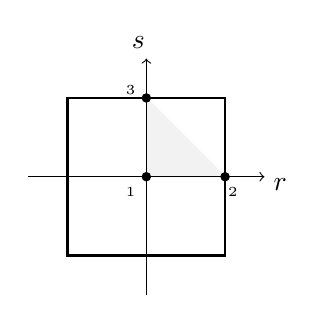
\begin{tikzpicture}
%\draw[step=0.5cm,gray,very thin] (0,0) grid (4,4); 
\draw[fill=gray!10,gray!10](2,2)--(3,2)--(2,3)--cycle;
\draw[thick] (1,1)--(3,1)--(3,3)--(1,3)--cycle;
\draw [->] (0.5,2) -- (3.5,2);
\draw [->] (2,0.5) -- (2,3.5);
\node[] at (3.7,1.9) {$r$};
\node[] at (1.9,3.7) {$s$};
\draw[black,fill=black] (2,2)   circle (1.5pt);
\draw[black,fill=black] (3,2)   circle (1.5pt);
\draw[black,fill=black] (2,3)   circle (1.5pt);
\node[] at (1.8,1.8) {\tiny $1$};
\node[] at (3.1,1.8) {\tiny $2$};
\node[] at (1.8,3.1) {\tiny $3$};
\end{tikzpicture}
\end{center}



and we would then have
\begin{mdframed}[backgroundcolor=blue!5]
\begin{eqnarray}
\bN_1(r) &=& 1-r-s  \nonumber\\
\bN_2(r) &=& r   \nonumber\\
\bN_3(r) &=& s
\end{eqnarray}
\end{mdframed}








%.....................................................................
\subsubsection{Enriched linear basis functions in triangles ($P_1^+$)}
\index{general}{$P_1^+$}

As we will see in Section~\ref{pair:mini} the above $P_1$ can be enriched 
with a so-called bubble function.
The \index{general}{Bubble Function} bubble function of the MINI element 
is described in \cite{arbf84} as being $\lambda_1\lambda_2\lambda_3$
where $\lambda_i$ are the so-called barycentric 
coordinates\footnote{\url{https://en.wikipedia.org/wiki/Barycentric\_coordinate\_system }}.
\index{general}{Barycentric Coordinates}

\begin{eqnarray}
\lambda_1 &=& \frac{(y2-y3)(x-x3)+(x3-x2)(y-y3)}{(y2-y3)(x1-x3)+(x3-x2)(y1-y3)} \nn\\
\lambda_2 &=& \frac{(y3-y1)(x-x3)+(x1-x3)(y-y3)}{(y2-y3)(x1-x3)+(x3-x2)(y1-y3)} \nn\\
\lambda_3 &=& 1-\lambda_1-\lambda_2 \nn
\end{eqnarray}

\begin{center}
\includegraphics[width=12cm]{images/mini/minielement2}\\
{\small representation of the element in the real coordinate system $(x,y)$
and in the reduced coordinate system $(r,s)$}
\end{center}

\begin{center}
\includegraphics[width=5cm]{images/mini/barycoord}\\
{\small Barycentric coordinates ($\lambda _{1},\lambda _{2},\lambda _{3}$) on an equilateral triangle and on a right triangle.}
\end{center}

In the reference triangle, the barycentric coordinates write
\begin{eqnarray}
\lambda_1 &=& \frac{(s_2-s_3)(r-r_3)+(r_3-r_2)(s-s_3)}{(s_2-s_3)(r_1-r_3)+(r_3-r_2)(s_1-s_3)} = \frac{(-1)(r)+(-1)(s-1)}{(-1)(0)+(-1)(-1)} = -r-s+1  \nn\\
\lambda_2 &=& \frac{(s3-s1)(r-r3)+(r1-r3)(s-s3)}{(s2-s3)(r1-r3)+(r3-r2)(s1-s3)} = \frac{(1)(r)+(0)(s-1)}{(-1)(0)+(-1)(-1)} = r \nn\\
\lambda_3 &=& 1-\lambda_1-\lambda_2 = 1 - (-r-s+1) - r = s \nn
\end{eqnarray}
As we have seen before the bubble function is given by $\lambda_1\lambda_2\lambda_3 = (1-r-s)rs$
and the polynomial form for the basis functions is given by:
\[
f(r,s) =a+br+cs + d (1-r-s)rs
\]
Setting the location of the bubble at $r=s=1/3$, i.e. $\lambda_1\lambda_2\lambda_3 = 1/3$, 
we then have 
\begin{eqnarray}
f(r_1,s_1)&=&f_1 = a+br_1+cs_1 + d (1-r_1-s_1)r_1s_1 = a \nn\\
f(r_2,s_2)&=&f_2 = a+br_2+cs_2 + d (1-r_2-s_2)r_2s_2 = a + b \nn\\
f(r_3,s_3)&=&f_3 = a+br_3+cs_3 + d (1-r_3-s_3)r_3s_3 = a + c \nn\\
f(r_4,s_4)&=&f_4 = a+br_4+cs_4 + d (1-r_4-s_4)r_4s_4 = a + \frac{b}{3} + \frac{c}{3} + \frac{1}{27} \nn
\end{eqnarray}
where point 4 is the location of the bubble.
This yields
\[
a=f_1 
\quad\quad\qquad
b=f_2-a = f_2-f_1
\quad\quad\qquad
c=f_3-a = f_3-f_1
\]
and
\[
d=27(f_4-a-\frac{b}{3} - \frac{c}{3}) = 27 (f_4 - f_1 - \frac{f_2-f_1}{3} - \frac{f_3-f_1}{3} )
=27(f_4 - \frac{f_1}{3}  - \frac{f_2}{3}  - \frac{f_3}{3} )
\] 

Finally
\begin{eqnarray}
f(r,s) 
&=&a+br+cs + d (1-r-s)rs \nn\\
&=& f_1 + (f_2-f_1)r + (f_3-f_1)s + 27(f_4 - \frac{f_1}{3}  - \frac{f_2}{3}  - \frac{f_3}{3} ) (1-r-s)rs \nn\\
&=& [1-r-s-9(1-r-s)rs] f_1 + [r-9(1-r-s)rs ]f_2 + [s-9(1-r-s)rs ]f_3 + [27(1-r-s)rs]f_4 \nn
\end{eqnarray}
so that 
\[
f(r,s)=\sum_{i=1}^4 N_i(r,s) f_i
\]
with 
%\begin{mdframed}[backgroundcolor=blue!15]
\begin{eqnarray}
N_1(r,s) &=& 1-r-s-9(1-r-s)rs \nn\\
N_2(r,s) &=& r-9(1-r-s)rs \nn\\
N_3(r,s) &=& s-9(1-r-s)rs \nn\\
N_4(r,s) &=& 27(1-r-s)rs \nn
\end{eqnarray}
%\end{mdframed}
It is trivial to verify that $\sum_i N_i =1$ for all values of $r,s$
and the gradients of the basis functions are:
\begin{eqnarray}
\frac{\partial N_1}{\partial r}(r,s) &=& -1 - 9(1-2r-s)s \\ 
\frac{\partial N_2}{\partial r}(r,s) &=&  +1 - 9(1-2r-s)s \\ 
\frac{\partial N_3}{\partial r}(r,s) &=&  - 9(1-2r-s)s \\ 
\frac{\partial N_4}{\partial r}(r,s) &=&  27(1-2r-s)s \\ 
\\
\frac{\partial N_1}{\partial s}(r,s) &=& -1 - 9(1-r-2s)r \\ 
\frac{\partial N_2}{\partial s}(r,s) &=&    - 9(1-r-2s)r \\ 
\frac{\partial N_3}{\partial s}(r,s) &=& +1 - 9(1-r-2s)r \\ 
\frac{\partial N_4}{\partial s}(r,s) &=&     27(1-r-2s)r 
\end{eqnarray}

We have two coordinate systems for the element: the global coordinates $(x,y)$ 
and the natural coordinates $(r,s)$. Inside the element, the relation between the two is given by
\begin{eqnarray}
x &=& N_1 x_1 + N_2 x_2 + N_3 x_3 + N_4 x_4 = \sum_i N_i(r,s) x_i\nn\\
y &=& N_1 y_1 + N_2 y_2 + N_3 y_3 + N_4 y_4 = \sum_i N_i(r,s) y_i
\end{eqnarray}
or,
\begin{eqnarray}
x &=& [ 1-r-s-9(1-r-s)rs] x_1 + [r-9(1-r-s)rs] x_2 + [s-9(1-r-s)rs] x_3 + [27(1-r-s)rs] x_4 \nn\\
&=& x_1 -r (x_1-x_2) -s (x_1-x_3) + (1-r-s)rs (-9 x_1 - 9 x_2  -9 x_3 +27 x_4)  \nn\\
&=& x_1 -r (x_1-x_2) -s (x_1-x_3) + (1-r-s)rs (-9 x_1 - 9 x_2  -9 x_3 +27 (x_1+x_2+x_3)/3) \nn\\ 
&=& x_1 -r (x_1-x_2) -s (x_1-x_3) \nn\\ 
&=& x_1 -r x_{12} -s x_{13} \nn\\ 
y &=& [ 1-r-s-9(1-r-s)rs] y_1 + [r-9(1-r-s)rs] y_2 + [s-9(1-r-s)rs] y_3 + [27(1-r-s)rs] y_4 \nn\\
&=& y_1 -r (y_1-y_2) -s (y_1-y_3) + (1-r-s)rs (-9 y_1 - 9 y_2  -9 y_3 +27 y_4)  \nn\\
&=& y_1 -r (y_1-y_2) -s (y_1-y_3) + (1-r-s)rs (-9 y_1 - 9 y_2  -9 y_3 +27 (y_1+y_2+y_3)/3) \nn\\ 
&=& y_1 -r (y_1-y_2) -s (y_1-y_3) \nn \\
&=& y_1 -r y_{12} -s y_{13} \nn 
\end{eqnarray}




























%%%%%%%%%%%%%%%%%%%%%%%%%%%%%%%%%%%%
\subsubsection{Quadratic basis functions for triangles in 2D ($P_2$)}
\index{general}{$P_2$}

\begin{verbatim}
2            
|\
| \        (r_0,s_0)=(0,0) (r_3,s_3)=(1/2,0)
5   4      (r_1,s_1)=(1,0) (r_4,s_4)=(1/2,1/2)
|     \    (r_2,s_2)=(0,1) (r_5,s_5)=(0,1/2)
|      \ 
0===3===1
\end{verbatim}
The basis polynomial is then
\[
f(r,s) = c_1 + c_2 r + c_3 s + c_4  r^2 + c_5 rs  + c_6 s^2
\]
We have 
\begin{eqnarray}
f_1 = f(r_1,s_1) &=& c_1 \nonumber\\
f_2 = f(r_2,s_2) &=& c_1 + c_2 + c_4\nonumber\\
f_3 = f(r_3,s_3) &=& c_1 + c_3 + c_6\nonumber\\
f_4 = f(r_4,s_4) &=& c_1 + c_2/2 + c_4/4\nonumber\\
f_5 = f(r_5,s_5) &=& c_1 + c_2/2 + c_3/2 \nonumber\\
                 &+& c_4/4 + c_5/4 + c_6/4\nonumber\\
f_6 = f(r_6,s_6) &=& c_1 + c_3/2 + c_6/4\nonumber
\end{eqnarray}

This can be cast as ${\bm f}={\bm A}\cdot {\bm c}$ where ${\bm A}$ is a 6x6 matrix:
\[
{\bm A}=
\left(
\begin{array}{cccccc}
1&0   &  0  & 0   & 0   & 0\\
1&1   &  0  & 1   & 0   & 0\\
1&0   &  1  & 0   & 0   & 1\\
1&1/2 &  0  & 1/4 & 0   & 0\\
1&1/2 &  1/2& 1/4 & 1/4 & 1/4\\
1&0   &  1/2& 0   & 0   & 1/4
\end{array}
\right)
\]
It is rather trivial to compute the inverse of this matrix:
\[
{\bm A}^{-1}=
\left(
\begin{array}{cccccc}
1  & 0 & 0  & 0  & 0 & 0  \\
-3 & -1& 0  & 4  & 0 & 0 \\
-3 & 0 & -1 & 0  & 0 & 4 \\
2  & 2 & 0  & -4 & 0 & 0  \\
4  & 0 & 0  & -4 & 4 & -4 \\
2  & 0 & 2  & 0  & 0 & -4
\end{array}
\right)
\]
In the end, one obtains:
\begin{eqnarray}
f(r,s) 
&=& f_1 + (-3f_1-f_2+4f_4) r + (-3f_1-f_3+4f_6)s \nonumber\\
&& +(2f_1+2f_2-4f_4)r^2 + (4f_1-4f_4+4f_5-4f_6) rs \nn\\
&&+ (2f_1+2f_3-4f_6)s^2 \nonumber\\
&=& \sum_{i=1}^6 N_i(r,s) f_i
\end{eqnarray}
with
\begin{mdframed}[backgroundcolor=blue!5]
\begin{eqnarray}
N_1(r,s) &=& 1-3r-3s+2r^2+4rs+2s^2 \nonumber\\
N_2(r,s) &=& -r+2r^2 \nonumber\\
N_3(r,s) &=& -s+2s^2 \nonumber\\
N_4(r,s) &=& 4r-4r^2-4rs \nonumber\\
N_5(r,s) &=& 4rs \nonumber\\
N_6(r,s) &=& 4s-4rs-4s^2 \nonumber
\end{eqnarray}
\end{mdframed}

The derivatives are as follows:
\begin{eqnarray}
\frac{\partial N_1}{\partial r}(r,s) &=&  -3+4r+4s \nn\\ 
\frac{\partial N_2}{\partial r}(r,s) &=&  -1+4r\nn\\ 
\frac{\partial N_3}{\partial r}(r,s) &=&  0\nn\\ 
\frac{\partial N_4}{\partial r}(r,s) &=&  4-8r-4s\nn\\ 
\frac{\partial N_5}{\partial r}(r,s) &=&  4s\nn\\ 
\frac{\partial N_6}{\partial r}(r,s) &=&  -4s\nn
\end{eqnarray}

\begin{eqnarray}
\frac{\partial N_1}{\partial s}(r,s) &=&  -3+4r+4s\nn\\ 
\frac{\partial N_2}{\partial s}(r,s) &=&  0\nn\\ 
\frac{\partial N_3}{\partial s}(r,s) &=&  -1+4s\nn\\ 
\frac{\partial N_4}{\partial s}(r,s) &=&  -4r\nn\\ 
\frac{\partial N_5}{\partial s}(r,s) &=&  4r\nn\\ 
\frac{\partial N_6}{\partial s}(r,s) &=&  4-4r-8s\nn
\end{eqnarray}



%.....................................................................
\subsubsection{Enriched quadratic basis functions in triangles ($P_2^+$)}
\index{general}{$P_2^+$}

This is used by the Crouzeix-Raviart element, see Section~\ref{sec:crouzeix-raviart}. 
\index{general}{Crouzeix-Raviart}

\begin{verbatim}
03             (r_1,s_1)=(0,0)
||\\           (r_2,s_2)=(1,0)
|| \\          (r_3,s_3)=(0,1)
||  \\         (r_4,s_4)=(1/2,0)
06   05        (r_5,s_5)=(1/2,1/2)
|| 07 \\       (r_6,s_6)=(0,1/2)
||     \\      (r_7,s_7)=(1/3,1/3)
01==04==02    
\end{verbatim}

The basis functions are given by:
\todo[inline]{find reference}

\begin{mdframed}[backgroundcolor=blue!5]
\begin{eqnarray}
N_1(r,s) &=&  (1-r-s)(1-2r-2s+ 3rs) \\
N_2(r,s) &=& r (2 r -1 + 3s-3rs-3s^2 ) \\
N_3(r,s) &=& s (2s -1 + 3r-3r^2-3rs )\\
N_4(r,s) &=& 4(1-r-s)r(1 -3s ) \\
N_5(r,s) &=& 4rs [-2+3r+3s]\\
N_6(r,s) &=& 4(1-r-s)s(1-3r)\\
N_7(r,s) &=& 27 (1-r-s)rs 
\end{eqnarray}
\end{mdframed}
It is then easy to verify that for all basis functions we have 
$N_i(r_j,s_j)=\delta_{ij}$ where $j$ denotes one of the seven nodes. 

The derivatives are as follows:
\begin{eqnarray}
\frac{\partial N_1}{\partial r}(r,s) &=& r(4-6s)-3s^2+7s-3\\
\frac{\partial N_2}{\partial r}(r,s) &=& r(4-6s)-3s^2+3s-1\\
\frac{\partial N_3}{\partial r}(r,s) &=& -3s(2r+s-1)  \\
\frac{\partial N_4}{\partial r}(r,s) &=& 4(3s-1)(2r+s-1) \\
\frac{\partial N_5}{\partial r}(r,s) &=& 4s(6r+3s-2) \\
\frac{\partial N_6}{\partial r}(r,s) &=& 4s(6r+3s-4)\\
\frac{\partial N_7}{\partial r}(r,s) &=& -27s(2r+s-1)
\end{eqnarray}

\begin{eqnarray}
\frac{\partial N_1}{\partial s}(r,s) &=& -3r^2+r(7-6s)+4s-3\\
\frac{\partial N_2}{\partial s}(r,s) &=& -3r(r+2s-1)\\
\frac{\partial N_3}{\partial s}(r,s) &=& -3r^2+r(3-6s)+4s-1 \\
\frac{\partial N_4}{\partial s}(r,s) &=& 4r(3r+6s-4)  \\
\frac{\partial N_5}{\partial s}(r,s) &=& 4r(3r+6s-2) \\
\frac{\partial N_6}{\partial s}(r,s) &=& 4(3r-1)(r+2s-1)\\
\frac{\partial N_7}{\partial s}(r,s) &=& -27r(r+2s-1)
\end{eqnarray}


Note that the basis functions can also be expressed as a function of the barycentric coordinates, 
as in the MILAMIN code \cite{daks08} or in Cuvelier \etal, 1986 \cite{cuss86}\footnote{Note
that the numbering of the nodes in the book is different with respect to the one above. }

\begin{verbatim}
03          
||\\        
|| \\       
||  \\      
05   04     
|| 07 \\    
||     \\   
01==06==02    
\end{verbatim}

\begin{eqnarray}
N_1(\lambda_1,\lambda_2,\lambda_3) &=& \eta_1(2\eta_1-1)+ 3\eta_1\eta_2\eta_3\\
N_2(\lambda_1,\lambda_2,\lambda_3) &=& \eta_2(2\eta_2-1)+ 3\eta_1\eta_2\eta_3\\
N_3(\lambda_1,\lambda_2,\lambda_3) &=& \eta_3(2\eta_3-1)+ 3\eta_1\eta_2\eta_3\\
N_4(\lambda_1,\lambda_2,\lambda_3) &=& 4\eta_2\eta_3 - 12\eta_1\eta_2\eta_3\\
N_5(\lambda_1,\lambda_2,\lambda_3) &=& 4\eta_1\eta_3 - 12\eta_1\eta_2\eta_3\\
N_6(\lambda_1,\lambda_2,\lambda_3) &=& 4\eta_1\eta_2 - 12\eta_1\eta_2\eta_3\\
N_7(\lambda_1,\lambda_2,\lambda_3) &=& 27\eta_1\eta_2\eta_3 
\end{eqnarray}

\todo[inline]{
VERIFY that when $\eta_1=1-r-s$, $\eta_2=r$ and $\eta_3=s$ we find the above $r,s$ basis functions
}


%1-4*eta1+3*eta1*eta3-3*eta2*eta3 ...
%-1+4*eta2+3*eta1*eta3-3*eta2*eta3 ...
%3*eta1*eta3-3*eta2*eta3 ...
%4*eta3+12*eta2*eta3-12*eta1*eta3 ...
%-4*eta3+12*eta2*eta3-12*eta1*eta3 ...
%4*eta1-4*eta2+12*eta2*eta3-12*eta1*eta3 ...
%-27*eta2*eta3+27*eta1*eta3

%1-4*eta1+3*eta1*eta2-3*eta2*eta3 ...
%+3*eta1*eta2-3*eta2*eta3 ...
%-1+4*eta3+3*eta1*eta2-3*eta2*eta3 ...
%4*eta2-12*eta1*eta2+12*eta2*eta3 ...
%4*eta1-4*eta3-12*eta1*eta2+12*eta2*eta3 ...
%-4*eta2-12*eta1*eta2+12*eta2*eta3 ...
%27*eta1*eta2-27*eta2*eta3];  







%%%%%%%%%%%%%%%%%%%%%%%%%%%%%%%%%%%%
\subsubsection{Cubic basis functions for triangles ($P_3$)}
\index{general}{$P_3$}

\begin{verbatim}
2
|\          (r_0,s_0)=(0,0)   (r_5,s_5)=(2/3,1/3)
|  \        (r_1,s_1)=(1,0)   (r_6,s_6)=(1/3,2/3)
7   6       (r_2,s_2)=(0,1)   (r_7,s_7)=(0,2/3)
|    \      (r_3,s_3)=(1/3,0) (r_8,s_8)=(0,1/3)
8  9   5    (r_4,s_4)=(2/3,0) (r_9,s_9)=(1/3,1/3)
|       \ 
0==3==4==1
\end{verbatim}
The basis polynomial is then
\[
f(r,s) = c_1 + c_2r + c_3s + c_4 r^2 + c_5 rs + c_6 s^2 + c_7 r^3 +c_8 r^2s + c_9 rs^2 + c_{10}s^3
\]
\begin{eqnarray}
N_0(r,s) &=& \frac{9}{2}(1-r-s)\left(\frac13-r-s\right)\left(\frac23-r-s\right) \\
N_1(r,s) &=& \frac{9}{2}r\left(r-\frac13\right)\left(r-\frac23 \right) \\
N_2(r,s) &=& \frac{9}{2}s\left(s-\frac13\right)\left(s-\frac23\right) \\
N_3(r,s) &=& \frac{27}{2}(1-r-s)r \left(\frac23-r-s\right) \\
N_4(r,s) &=& \frac{27}{2}(1-r-s)r\left(r-\frac13\right) \\
N_5(r,s) &=& \frac{27}{2}rs\left(r-\frac13\right) \\
N_6(r,s) &=& \frac{27}{2}rs\left(r-\frac23\right) \\
N_7(r,s) &=& \frac{27}{2}(1-r-s)s\left(s-\frac13\right) \\
N_8(r,s) &=& \frac{27}{2}(1-r-s)s \left(\frac23-r-s\right) \\
N_9(r,s) &=& 27 rs(1-r-s)
\end{eqnarray}



%..........................................................................
\subsubsection{Enriched linear basis functions in quadrilaterals ($Q_1^+$) -WIP} \label{ss:quadmini}
\index{general}{$Q_1^+$}

\begin{verbatim}
4===========3
|           |   (r_1,s_1)=(-1,-1)
|           |   (r_2,s_2)=(1,-1)
|     5     |   (r_3,s_3)=(1,1)
|           |   (r_4,s_4)=(-1,1)
|           |   (r_5,s_5)=(0,0)
1===========2
\end{verbatim}

\begin{itemize}
\item 
In Bai (1997) \cite{bai97}: "It is well known that the equal-order bilinear velocity-bilinear 
continuous pressure element - the $Q_1\times Q_1$, element - exhibits a certain spurious pressure mode.
In the paper we propose a new stabilized $Q_1\times Q_1$ combination for the velocity and
pressure with three internal degrees of freedom added to the velocity space, that is, one degree of
freedom for each component of the velocity and one degree of freedom shared by both components of
the velocity."

Two versions are proposed, if I understand it correctly.
The first one is given in Eq.~7 (three extra dofs: $u_5$, $v_5$, $w$):
\begin{eqnarray}
u^h(r,s) &=& \sum_{i=1}^4 N_i (r,s) u_i + \left[ u_5 - \frac{w}{4}(1-s) \right] (1-r^2)(1-s^2) \nonumber\\
v^h(r,s) &=& \sum_{i=1}^4 N_i (r,s) v_i + \left[ v_5 - \frac{w}{4}(1-r) \right] (1-r^2)(1-s^2) 
\end{eqnarray}
The second one in Eq.23 (four extra dofs: $u_5$, $v_5$, $u_6$, $v_6$):
\begin{eqnarray}
u^h(r,s) &=& \sum_{i=1}^4 N_i (r,s) u_i + \left[ u_5 +u_6(r+s) \right] (1-r^2)(1-s^2) \nonumber\\
v^h(r,s) &=& \sum_{i=1}^4 N_i (r,s) v_i + \left[ v_5 +v_6(r+s) \right] (1-r^2)(1-s^2) 
\end{eqnarray}

\item In Franca \etal (2007) \cite{fros07}: 
"Stabilized finite element method for Stokes equations with piecewise continuous 
bilinear approximations for both velocity and pressure variables. The velocity
field is enriched with piecewise polynomial bubble functions with null average at element
edges."

It looks like they are proposing (see their Eq.~2.6):
\begin{eqnarray}
u^h(r,s) &=& \sum_{i=1}^4 N_i (r,s) u_i + (\alpha + \gamma s)\frac{1}{2}(r^2+s^2-\frac43) \nn\\ 
v^h(r,s) &=& \sum_{i=1}^4 N_i (r,s) v_i + (\beta + \gamma r) \frac{1}{2}(r^2+s^2-\frac43)  
\end{eqnarray}

\item In Kwon \& Park \cite{kwpa14}: 
"We introduce a new stable MINI-element pair for incompressible Stokes equations on
quadrilateral meshes, which uses the smallest number of bubbles for the velocity. The pressure is 
discretized with the $P_1$-midpoint-edge-continuous elements and each component of the velocity field is
done with the standard $Q_1$-conforming elements enriched by one bubble a quadrilateral."

\item  In Lamichhane (2017) \cite{lami17}: "We consider a quadrilateral MINI
finite element for approximating the solution
of Stokes equations using a quadrilateral mesh. We use the standard bilinear finite
element space enriched with element-wise defined bubble functions for the velocity
and the standard bilinear finite element space for the pressure space. With a simple
modification of the standard bubble function we show that a single bubble function is
sufficient to ensure the inf-sup condition.
This is a refinement of \cite{bai97} where the author enriches the velocity space with
more than a single vector bubble function per element. In this article we show that 
with a small modification of the standard bubble function we can get the stability just 
by using a single vector bubble function per element."

\input{lamichhane2D}

\end{itemize}


\Literature Mons \& Roge (1992) \cite{moro92}, 
Li \etal (2009) \cite{lihc09}, Knobloch \& Tobiska (2000) \cite{knto00}, 
Franca \etal (1993) \cite{frha93}, Idelsohn \etal (1995) \cite{idsn95}.





\newpage
%-----------------------------------------------------------------
\subsubsection{The rotated $Q_1$} \label{ss:rq1}
\index{general}{$\tilde{Q}_1$}

The nodes are not on the corners of the element but in the middle of the
element edges:

\begin{flushright} {\tiny {\color{gray} (tikz\_RTQ1P0.tex)}} \end{flushright}
%~~~~~~~~~~~~~~~~~~~~~~~~~~~~~~~~~~~~~~~~~~~~~~~~~~~~~~~~~~~~~~~~~~~~~~~~~~~~~~~~~~~~~~~~~~~~~~~~~~

\begin{center}
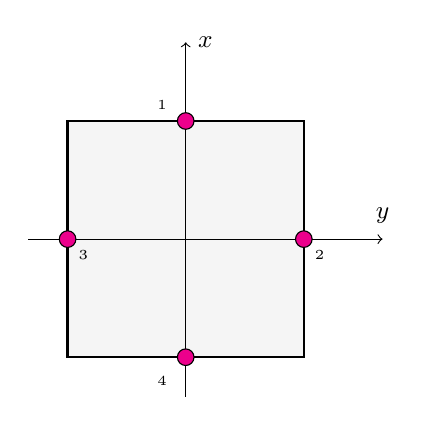
\begin{tikzpicture}
%\draw[step=1cm,gray,very thin] (0,0) grid (8,8); %background grid

\draw[thick,fill=gray!8] (1,1) -- (4,1) -- (4,4) -- (1,4) -- cycle;

\node[] at (1.2,2.3) {\tiny 3};
\node[] at (4.2,2.3) {\tiny 2};
\node[] at (2.2,.7) {\tiny 4};
\node[] at (2.2,4.2) {\tiny 1};

\draw[->] (0.5,2.5)--(5,2.5);
\draw[->] (2.5,0.5)--(2.5,5);

\draw[black,fill=magenta] (1,2.5)   circle (3pt);
\draw[black,fill=magenta] (4,2.5)   circle (3pt);
\draw[black,fill=magenta] (2.5,1)   circle (3pt);
\draw[black,fill=magenta] (2.5,4)   circle (3pt);

\node[] at (5,2.8) {\small $y$};
\node[] at (2.75,5) {\small $x$};
\end{tikzpicture}
\end{center}




\begin{verbatim}
+======3======+
|             |
|      s      |
|      |      |
4      +--r   2
|             |
|             |
|             |
+======1======+
\end{verbatim}

There are two types of basis functions: the Middle Point (MP) variant
such that $N_i({\bm r}_j)=\delta_{ij}$ and the Mid Value (MV) variant
such that $\frac{1}{|\Gamma_i|} \int_{\Gamma_i} N_j d\Gamma = \delta_{ij}$.

%.............................................
\paragraph{The Middle Point (MP) variant}. 
We have $\tilde{Q}_1=span \{ 1,r,s,r^2-s^2 \}$
so a function $f \in \tilde{Q}_1$  is such that 
\begin{equation}
f(r,s)= a + b r + c s + d(r^2-s^2 )
\label{nonpsf}
\end{equation}

This function must be so that 
\begin{eqnarray}
f_1 &=& f(r=0 ,s=-1) = a -c -d \\
f_2 &=& f(r=+1,s=0)  = a +b +d \\
f_3 &=& f(r=0 ,s=+1) = a +c -d \\
f_4 &=& f(r=-1,s=0)  = a -b +d 
\end{eqnarray}
and then 
\[
\left(
\begin{array}{c}
f_A \\ f_b \\ f_C \\ f_D
\end{array}
\right)
=
\left(
\begin{array}{cccc}
1 &0 &-1 &-1 \\
1 &1 &0 &1 \\
1 &0 &1 &-1 \\
1 &-1 &0 &1
\end{array}
\right)
\left(
\begin{array}{c}
a \\ b \\ c \\ d
\end{array}
\right)
\]
This system can easily be solved, $a,b,c,d$ are then replaced in Eq.~\eqref{nonpsf},
which yields 
\begin{eqnarray}
f(r,t) &=& N_1(r,s)f_1 +N_2(r,s)f_1 + N_3(r,s)f_3 +N_4(r,s)f_4
\end{eqnarray}
inside the element with
\begin{mdframed}[backgroundcolor=blue!5]
\begin{eqnarray}
N_1(r,s) &=& \frac{1}{4} (1-2s-(r^2-s^2)) \nonumber\\
N_2(r,s) &=& \frac{1}{4} (1+2r+(r^2-s^2)) \nonumber\\
N_3(r,s) &=& \frac{1}{4} (1+2s-(r^2-s^2)) \nonumber\\
N_4(r,s) &=& \frac{1}{4} (1-2r+(r^2-s^2)) \nonumber
\end{eqnarray}
\end{mdframed}
We of course recover the partition of unity property, i.e. $\sum N_i(r,s)=1$ for any coordinate $r,s$ inside 
the reference element.

\begin{remark}
These basis functions have been independently proposed by Donea \etal. \cite{dogm81}. The authors
prove herein that this element is checkerboard-free (although they do no show any example
of simulation carried out with this element).
\end{remark}

\begin{eqnarray}
\frac{\partial N_1}{\partial r} &=& \frac{1}{2}(-r)\\
\frac{\partial N_2}{\partial r} &=& \frac{1}{2}(1+r)\\
\frac{\partial N_3}{\partial r} &=& \frac{1}{2}(-r)\\
\frac{\partial N_4}{\partial r} &=& \frac{1}{2}(-1+r)
\end{eqnarray}

\begin{eqnarray}
\frac{\partial N_1}{\partial s} &=& \frac{1}{2}(-1+s)\\
\frac{\partial N_2}{\partial s} &=& \frac{1}{2}(-s)\\
\frac{\partial N_3}{\partial s} &=& \frac{1}{2}(1+s)\\
\frac{\partial N_4}{\partial s} &=& \frac{1}{2}(-s)
\end{eqnarray}

\begin{center}
\includegraphics[width=6cm]{images/rannacherturek/N1}
\includegraphics[width=6cm]{images/rannacherturek/N2}\\
\includegraphics[width=6cm]{images/rannacherturek/N3}
\includegraphics[width=6cm]{images/rannacherturek/N4}\\
{\captionfont Graphical representation of the $\tilde{Q}_1$ basis functions}
\end{center}

%......................................
\paragraph{The Mid Value (MV) variant}. 

These basis functions are implemented in deal.II
\footnote{\url{https://www.dealii.org/8.5.0/doxygen/deal.II/polynomials_rannacher_turek_8cc_source.html}}
for $x\in[0,1]$ and $y\in[0,1]$:

\begin{eqnarray}
N_1(x,y) &=&  0.75 + 1.5x - 2.5y -1.5(x^2-y^2) \quad bottom\\
N_2(x,y) &=& -0.25 - 0.5x + 1.5y +1.5(x^2-y^2) \quad right\\
N_3(x,y) &=& -0.25 + 1.5x - 0.5y -1.5(x^2-y^2) \quad top\\
N_4(x,y) &=&  0.75 - 2.5x + 1.5y +1.5(x^2-y^2) \quad left
\end{eqnarray}
We then proceed to rewrite these for $r\in[-1,1]$ and $t\in[-1:1]$:
\begin{mdframed}[backgroundcolor=blue!5]
\begin{eqnarray}
N_1(r,s) &=& \frac{1}{4} -\frac{1}{2}s - \frac{3}{8}(r^2-s^2) \quad bottom \\
N_2(r,s) &=& \frac{1}{4} +\frac{1}{2}r + \frac{3}{8}(r^2-s^2) \quad right \\
N_3(r,s) &=& \frac{1}{4} +\frac{1}{2}s - \frac{3}{8}(r^2-s^2) \quad top \\
N_4(r,s) &=& \frac{1}{4} -\frac{1}{2}r + \frac{3}{8}(r^2-s^2) \quad left
\end{eqnarray}
\end{mdframed}
It is easy to verify that these functions verify the property
\[
\frac{1}{|\Gamma_i|} \int_{\Gamma_i} N_j d\Gamma = \delta_{ij}
\]

These basis functions are used in \cite{shzh06} and mentioned in John \cite[p.722]{john16}.

\begin{eqnarray}
\frac{\partial N_1}{\partial r} &=& -\frac{3}{4}r \nonumber\\
\frac{\partial N_2}{\partial r} &=& \frac{1}{2}+\frac{3}{4}r \nonumber\\
\frac{\partial N_3}{\partial r} &=& -\frac{3}{4}r \nonumber\\
\frac{\partial N_4}{\partial r} &=& -\frac{1}{2}+\frac{3}{4}r \nonumber
\end{eqnarray}

\begin{eqnarray}
\frac{\partial N_1}{\partial t} &=& -\frac{1}{2}+\frac{3}{4}t \nonumber\\
\frac{\partial N_2}{\partial t} &=& -\frac{3}{4}t \nonumber\\
\frac{\partial N_3}{\partial t} &=& \frac{1}{2}+\frac{3}{4}t \nonumber\\
\frac{\partial N_4}{\partial t} &=& -\frac{3}{4}t \nonumber
\end{eqnarray}


\newpage
%-----------------------------------------------------------------------------
\subsubsection{The 2D enriched $Q_1^+\times P_0$ of Fortin} \label{ss:Q1pP02D}

We here consider the enriched $Q_1\times P_0$ element introduced first by 
Fortin (1981) \cite{fort81}.
The layout of the degrees of freedom is as follows:

\begin{flushright} {\tiny {\color{gray} (tikz\_q1pp02D.tex)}} \end{flushright}
%~~~~~~~~~~~~~~~~~~~~~~~~~~~~~~~~~~~~~~~~~~~~~~~~~~~~~~~~~~~~~~~~~~~~~~~~~~~~~~~~~~~~~~~~~~~~~~~~~~

\begin{center}
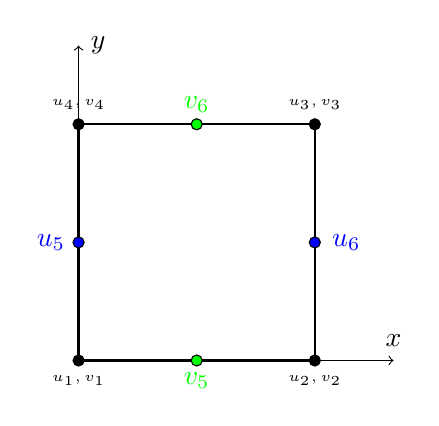
\begin{tikzpicture}
%\draw[fill=gray!23,gray!23](0,0) rectangle (6,5);
%\draw[step=0.5cm,gray,very thin] (0,0) grid (6,5); %background grid

\draw[thick] (1,.5) -- (4,.5) -- (4,3.5) -- (1,3.5) -- cycle; %front

\draw[thin,->] (4,0.5) -- (5,0.5); %x
\draw[thin,->] (1,3.5) -- (1,4.5); %y
\node[] at (5,0.75) {$x$};
\node[] at (1.25,4.5) {$y$};

\draw[black,fill=black] (1,.5)   circle (2pt);
\draw[black,fill=black] (4,.5)   circle (2pt);
\draw[black,fill=black] (4,3.5)   circle (2pt);
\draw[black,fill=black] (1,3.5)   circle (2pt);

\node[] at (1,0.25) {\tiny $u_1,v_1$};
\node[] at (4,0.25) {\tiny $u_2,v_2$};
\node[] at (4,3.75) {\tiny $u_3,v_3$};
\node[] at (1,3.75) {\tiny $u_4,v_4$};

\draw[black,fill=blue] (1,2) circle (2pt); 
\draw[black,fill=blue] (4,2) circle (2pt); 
\node[] at (0.65,2) {\color{blue} $u_5$};
\node[] at (4.4,2) {\color{blue} $u_{6}$};

\draw[black,fill=green] (2.5,0.5) circle (2pt); 
\draw[black,fill=green] (2.5,3.5) circle (2pt); 
\node[] at (2.5,0.25) {\color{green} $v_5$};
\node[] at (2.5,3.75) {\color{green} $v_{6}$};

\end{tikzpicture}\\
\end{center}


\noindent The approximation of the velocity components $u$ and $v$ inside the element is
\[
u^h(r,s) = a^u \; N_1(r,s) + b^u \;  N_2(r,s) + c^u \; N_3(r,s) +d^u \; N_4(r,s) 
+ d\; b_5^u(r,s) + e\; b_{6}^u(r,s)
\]
\[
v^h(r,s) = a^v \; N_1(r,s) + b^v \;  N_2(r,s) + c^v \; N_3(r,s) +d^v \; N_4(r,s) 
+ d^v b_5^v(r,s) + e^v b_{6}^v(r,s)
\]
where $N_{1,2,3,4}$ are the standard $Q_1$ basis functions in 2D and with 
\[
b_5^u(r,s) = \frac{1}{2}(1-r)(1-s^2)
\qquad
b_6^u(r,s) = \frac{1}{2}(1+r)(1-s^2)
\]
and
\[
b_5^v(r,s) = \frac{1}{2}(1-r^2)(1-s)
\qquad
b_6^v(r,s) = \frac{1}{2}(1-r^2)(1+s)
\]
In the end one arrives at

\begin{mdframed}[backgroundcolor=blue!5]
\begin{eqnarray}
{N}_1^u(r,s) &=&  N_1(r,s) - \frac{1}{2} b_5^u(r,s)\nn\\
{N}_2^u(r,s) &=&  N_2(r,s) - \frac{1}{2} b_6^u(r,s)\nn\\
{N}_3^u(r,s) &=&  N_3(r,s) - \frac{1}{2} b_6^u(r,s)\nn\\
{N}_4^u(r,s) &=&  N_4(r,s) - \frac{1}{2} b_5^u(r,s)\nn\\
{N}_5^u(r,s) &=&  b_5^u(r,s) \nn\\
{N}_6^u(r,s) &=&  b_6^u(r,s) \nn\\
\nn\\
{N}_1^v(r,s) &=&  N_1(r,s) - \frac{1}{2} b_5^v(r,s)\nn\\
{N}_2^v(r,s) &=&  N_2(r,s) - \frac{1}{2} b_5^v(r,s)\nn\\
{N}_3^v(r,s) &=&  N_3(r,s) - \frac{1}{2} b_6^v(r,s)\nn\\
{N}_4^v(r,s) &=&  N_4(r,s) - \frac{1}{2} b_6^v(r,s)\nn\\
{N}_5^v(r,s) &=&  b_5^v(r,s) \nn\\
{N}_6^v(r,s) &=&  b_6^v(r,s) 
\end{eqnarray}
\end{mdframed}

We can check for the zero-th order consistency: Let $u(r,s)=C$, then 
\begin{eqnarray}
u^h(r,s) 
= \sum_{i=1}^6 N_i^u(r,s) u_i 
= C \sum_{i=1}^6 N_i^u(r,s) 
= C \sum_{i=1}^4 N_i(r,s)  
= C
\end{eqnarray}



\newpage
%-----------------------------------------------------------------------------
\subsubsection{The DSSY element} \label{ss:dssy_2D}
This element is often reffered to as the 'DSSY' element becaus of the 
four authors of the original paper: Douglas, Santos, sheen and Ye (1999) \cite{doss99}.

The non-conforming finite element space i$Q_l$ is defined based on the 
reference square element on $[-1,1]^2$ :
\[
Q_l = \text{Span} \left\{ 1, r, s, \theta_l(r)-\theta_l(s)  \right\}
\qquad l=1,\; \text{or} \; 2
\]
with
\begin{eqnarray}
\theta_1(r)  &=& r^2-\frac53r^4  \nn\\
\theta_1'(r) &=& 2r-\frac{20}{3}r^3  \nn\\
\theta_2(r)  &=& r^2-\frac{25}{6} r^4 + \frac72 r^6 \\ 
\theta_2'(r) &=& 2r-\frac{50}{3} r^3 + 21 r^5
\end{eqnarray}
The dimension of $Q_l$ is four and the $\theta_l$ functions look like:
\begin{center}
\includegraphics[width=7cm]{images/dssy/theta1}
\includegraphics[width=7cm]{images/dssy/theta2}
\end{center}
We have:
\begin{itemize}
\item $\theta_1(r=-1)=\theta_1(r=+1)=-\frac23$, $\theta_1(r=0)=0$ 
\item $\theta_2(r=-1)=\theta_2(r=+1)=\frac13$, $\theta_2(r=0)=0$ 
\end{itemize}
The nodes are situated at the mid-edges of the quadrilateral:

\input{tikz_dssy2D}

The basis function corresponding to the node (1, 0) is given by
\begin{mdframed}[backgroundcolor=blue!5]
\begin{eqnarray}
N_1(r,s)^{(l)} &=& \frac{1}{4} - \frac{1}{2} r + \frac{\theta_l(r)-\theta_l(s)}{4 \theta_l(1)}  \nn\\
N_2(r,s)^{(l)} &=& \frac{1}{4} + \frac{1}{2} r + \frac{\theta_l(r)-\theta_l(s)}{4 \theta_l(1)}  \nn\\
N_3(r,s)^{(l)} &=& \frac{1}{4} - \frac{1}{2} s - \frac{\theta_l(r)-\theta_l(s)}{4 \theta_l(1)}  \nn\\
N_4(r,s)^{(l)} &=& \frac{1}{4} + \frac{1}{2} s - \frac{\theta_l(r)-\theta_l(s)}{4 \theta_l(1)}  
\end{eqnarray}
\end{mdframed}
We can easily verify that $\sum_i N_i(r,s,t)=1$ and that $N_i(\vec{r}_j)=\delta_{ij}$:
\begin{eqnarray}
N_1^{(l)}(r_1,s_1) 
&=& \frac{1}{4} -\frac{1}{2} (-1) + \frac{\theta_l(-1)-\theta_l(0)}{4 \theta_l(1)}  
= \frac{1}{4} +\frac{1}{2}  + \frac{\theta_l(-1)}{4 \theta_l(1)}  
= \frac{1}{4} +\frac{1}{2}  + \frac{1}{4}   = 1 \nn\\
N_1^{(l)}(r_2,s_2)
&=& \frac{1}{4} -\frac{1}{2} (+1) + \frac{\theta_l(+1)-\theta_l(0)}{4 \theta_l(1)}  
= \frac{1}{4} -\frac{1}{2} + \frac{\theta_l(+1)}{4 \theta_l(1)}  
= \frac{1}{4} -\frac{1}{2} + \frac{1}{4}   = 0 \nn\\
N_1^{(l)}(r_3,s_3)
&=& \frac{1}{4} -\frac{1}{2} (0) + \frac{\theta_l(0)-\theta_l(-1)}{4 \theta_l(1)}  
= \frac14 -\frac14  = 0 \nn\\
N_1^{(l)}(r_4,s_4)
&=& \frac{1}{4} -\frac{1}{2} (0) + \frac{\theta_l(0)-\theta_l(+1)}{4 \theta_l(1)}  
= \frac14 -\frac14  = 0 \nn\\
N_2^{(l)}(r_1,s_1) 
&=& \frac{1}{4} + \frac{1}{2} (-1) + \frac{\theta_l(-1)-\theta_l(0)}{4 \theta_l(1)}  
= \frac14 -\frac12 + \frac14 = 0 \nn\\
N_2^{(l)}(r_2,s_2)
&=& \frac{1}{4} + \frac{1}{2} (+1) + \frac{\theta_l(+1)-\theta_l(0)}{4 \theta_l(1)}  
= \frac14 + \frac12 + \frac14 =1 \nn\\
N_2^{(l)}(r_3,s_3)
&=& \frac{1}{4} + \frac{1}{2} (0) + \frac{\theta_l(0)-\theta_l(-1)}{4 \theta_l(1)}  
= \frac14 - \frac14 = 0 \nn\\
N_2^{(l)}(r_4,s_4)
&=& \frac{1}{4} + \frac{1}{2} (0) + \frac{\theta_l(0)-\theta_l(+1)}{4 \theta_l(1)}  
= \frac14 - \frac14 = 0 \nn\\
N_3^{(l)}(r_1,s_1)
&=& \frac{1}{4} - \frac{1}{2} (0) - \frac{\theta_l(-1)-\theta_l(0)}{4 \theta_l(1)} 
= \frac14 -\frac14 = 0\nn\\
N_3^{(l)}(r_2,s_2)
&=& \frac{1}{4} - \frac{1}{2} (0) - \frac{\theta_l(+1)-\theta_l(0)}{4 \theta_l(1)} 
= \frac14 -\frac14 = 0\nn\\
N_3^{(l)}(r_3,s_3)
&=& \frac{1}{4} - \frac{1}{2} (-1) - \frac{\theta_l(0)-\theta_l(-1)}{4 \theta_l(1)} 
= \frac14 +\frac12 + \frac14 = 1\nn\\
N_3^{(l)}(r_4,s_4)
&=& \frac{1}{4} - \frac{1}{2} (+1) - \frac{\theta_l(0)-\theta_l(+1)}{4 \theta_l(1)} 
= \frac14 -\frac12 + \frac14 = 0\nn\\
N_4^{(l)}(r_1,s_1)
&=& \frac{1}{4} + \frac{1}{2} (0) - \frac{\theta_l(-1)-\theta_l(0)}{4 \theta_l(1)}  
= \frac14 -\frac14 =0\nn\\
N_4^{(l)}(r_2,s_2)
&=& \frac{1}{4} + \frac{1}{2} (0) - \frac{\theta_l(+1)-\theta_l(0)}{4 \theta_l(1)}  
= \frac14 -\frac14 =0\nn\\
N_4^{(l)}(r_3,s_3)
&=& \frac{1}{4} + \frac{1}{2} (-1) - \frac{\theta_l(0)-\theta_l(-1)}{4 \theta_l(1)}  
= \frac14 -\frac12 +\frac14 = 0 \nn\\
N_4^{(l)}(r_4,s_4)
&=& \frac{1}{4} + \frac{1}{2} (1) - \frac{\theta_l(0)-\theta_l(1)}{4 \theta_l(1)}  
= \frac14 +\frac12 +\frac14 = 1 \nn
\end{eqnarray}

The basis functions can also be explicitely written for $\theta_1$ as in Cai \etal \cite{cady99}:
\begin{eqnarray}
N_1(r,s)^{(l)} 
&=& \frac{1}{4} - \frac{1}{2} r - \frac38 \left[\left( r^2-\frac53r^4 \right) - \left(s^2-\frac53s^4 \right) \right] \nn\\
N_2(r,s)^{(l)} 
&=& \frac{1}{4} + \frac{1}{2} r - \frac38 \left[\left( r^2-\frac53r^4 \right) - \left(s^2-\frac53s^4 \right) \right] \nn\\
N_3(r,s)^{(l)} 
&=& \frac{1}{4} - \frac{1}{2} s + \frac38 \left[\left( r^2-\frac53r^4 \right) - \left(s^2-\frac53s^4 \right) \right] \nn\\
N_4(r,s)^{(l)} 
&=& \frac{1}{4} + \frac{1}{2} s + \frac38 \left[\left( r^2-\frac53r^4 \right) - \left(s^2-\frac53s^4 \right) \right] 
\end{eqnarray}

The derivatives of the basis functions are as follows:
\begin{eqnarray}
\partial_r N_1(r,s)^{(l)} &=&  - \frac{1}{2}  + \frac{\theta_l'(r)}{4 \theta_l(1)}  \nn\\
\partial_r N_2(r,s)^{(l)} &=&  + \frac{1}{2}  + \frac{\theta_l'(r)}{4 \theta_l(1)}  \nn\\
\partial_r N_3(r,s)^{(l)} &=&  - \frac{\theta_l'(r)}{4 \theta_l(1)}  \nn\\
\partial_r N_4(r,s)^{(l)} &=&  - \frac{\theta_l'(r)}{4 \theta_l(1)}  
\end{eqnarray}

\begin{eqnarray}
\partial_s N_1(r,s)^{(l)} &=&   -\frac{\theta_l'(s)}{4 \theta_l(1)}  \nn\\
\partial_s N_2(r,s)^{(l)} &=&   -\frac{\theta_l'(s)}{4 \theta_l(1)}  \nn\\
\partial_s N_3(r,s)^{(l)} &=&   - \frac{1}{2} + \frac{\theta_l'(s)}{4 \theta_l(1)}  \nn\\
\partial_s N_4(r,s)^{(l)} &=&   + \frac{1}{2} + \frac{\theta_l'(s)}{4 \theta_l(1)}  
\end{eqnarray}





\Literature: 
Jeon \etal (2013) \cite{jens13},
Bangerth \etal (2017) \cite{baks17},
Sheen (2020) \cite{shee20}













 %-----------
\newpage
\subsection{Elements and basis functions in 3D} 

%%%%%%%%%%%%%%%%%%%%%%%%%%%%%%%%%%%%%%%%%%%%%%%%%%%%%%%
\subsubsection{Linear basis functions in tetrahedra ($P_1$)}
\index{$P_1$}


\begin{verbatim}
(r_0,s_0) = (0,0,0)
(r_1,s_1) = (1,0,0)
(r_2,s_2) = (0,2,0)
(r_3,s_3) = (0,0,1)
\end{verbatim}

The basis polynomial is given by
\[
f(r,s,t)=c_0 + c_1 r + c_2 s + c_3 t
\]

\begin{eqnarray}
f_1 &=& f(r_1,s_1,t_1) = c_0 \\
f_2 &=& f(r_2,s_2,t_2) = c_0 + c_1\\
f_3 &=& f(r_3,s_3,t_3) = c_0 + c_2\\
f_4 &=& f(r_4,s_4,t_4) = c_0 + c_3
\end{eqnarray}

which yields:
\[
c_0=f_1
\quad
\quad
c_1=f_2-f_1
\quad
\quad
c_2=f_3-f_1
\quad
\quad
c_3=f_4-f_1
\]

\begin{eqnarray}
f(r,s,t) 
&=& c_0 + c_1 r + c_2 s + c_3 t \nonumber\\
&=& f_1 + (f_2-f_1) r + (f_3-f_1) s + (f_4-f_1) t \nonumber\\
&=& f_1 (1-r-s-t) + f_2 r + f_3 s + f_4 t \nonumber\\
&=& \sum_i N_i(r,s,t) f_i \nonumber
\end{eqnarray}

Finally,

\begin{mdframed}[backgroundcolor=blue!5]
\begin{eqnarray}
N_1(r,s,t) &=& 1-r-s-t \nonumber\\
N_2(r,s,t) &=& r \nonumber\\
N_3(r,s,t) &=& s \nonumber\\
N_4(r,s,t) &=& t \nonumber
\end{eqnarray}
\end{mdframed}









%%%%%%%%%%%%%%%%%%%%%%%%%%%%%%%%%%%%%%%%%%%%%%%%%%%%%%%
\subsubsection{Triquadratic basis functions in 3D ($Q_2$)}
\index{$Q_2$}

\begin{eqnarray}
N_{1}&=& 0.5r(r-1)  \;0.5s(s-1)\; 0.5t(t-1)  \nonumber\\
N_{2}&=& 0.5r(r+1)  \;0.5s(s-1)\; 0.5t(t-1)  \nonumber\\
N_{3}&=& 0.5r(r+1)  \;0.5s(s+1)\; 0.5t(t-1)  \nonumber\\
N_{4}&=& 0.5r(r-1)  \;0.5s(s+1)\; 0.5t(t-1)  \nonumber\\
N_{5}&=& 0.5r(r-1)  \;0.5s(s-1)\; 0.5t(t+1)  \nonumber\\
N_{6}&=& 0.5r(r+1)  \;0.5s(s-1)\; 0.5t(t+1)  \nonumber\\
N_{7}&=& 0.5r(r+1)  \;0.5s(s+1)\; 0.5t(t+1)  \nonumber\\
N_{8}&=& 0.5r(r-1)  \;0.5s(s+1)\; 0.5t(t+1)  \nonumber\\
N_{9}&=& (1.-r^2)   \;0.5s(s-1)\; 0.5t(t-1)  \nonumber\\
N_{10}&=& 0.5r(r+1) \;(1-s^2)  \; 0.5t(t-1)  \nonumber\\
N_{11}&=& (1.-r^2)  \;0.5s(s+1)\; 0.5t(t-1)  \nonumber\\
N_{12}&=& 0.5r(r-1) \;(1-s^2)  \; 0.5t(t-1)  \nonumber\\
N_{13}&=& (1.-r^2)  \;0.5s(s-1)\; 0.5t(t+1)  \nonumber\\
N_{14}&=& 0.5r(r+1) \;(1-s^2)  \; 0.5t(t+1)  \nonumber\\
N_{15}&=& (1.-r^2)  \;0.5s(s+1)\; 0.5t(t+1)  \nonumber\\
N_{16}&=& 0.5r(r-1) \;(1-s^2)  \; 0.5t(t+1)  \nonumber\\
N_{17}&=& 0.5r(r-1) \;0.5s(s-1)\; (1-t^2)  \nonumber\\
N_{18}&=& 0.5r(r+1) \;0.5s(s-1)\; (1-t^2)  \nonumber\\
N_{19}&=& 0.5r(r+1) \;0.5s(s+1)\; (1-t^2)  \nonumber\\
N_{20}&=& 0.5r(r-1) \;0.5s(s+1)\; (1-t^2)  \nonumber\\
N_{21}&=& (1-r^2)   \;(1-s^2)  \; 0.5t(t-1)  \nonumber\\
N_{22}&=& (1-r^2)   \;0.5s(s-1)\; (1-t^2)  \nonumber\\
N_{23}&=& 0.5r(r+1) \;(1-s^2)  \; (1-t^2)  \nonumber\\
N_{24}&=& (1-r^2)   \;0.5s(s+1)\; (1-t^2)  \nonumber\\
N_{25}&=& 0.5r(r-1) \;(1-s^2)  \; (1-t^2)  \nonumber\\
N_{26}&=& (1-r^2)   \;(1-s^2)  \; 0.5t(t+1)  \nonumber\\
N_{27}&=& (1-r^2)   \;(1-s^2)  \; (1-t^2)  \nonumber
\end{eqnarray}

 %-------------------------------
\subsection{Low order elements recap} Let us assume a Cartesian domain discretised in $nel_x \times nel_y$
elements in 2D and $nel_x \times nel_y \times nel_z$ elements in 3D.
Focusing only on the total number of velocity dofs (the values indicated after the 
arrows are the limits when $nel_x=nel_y=nel_z >> 1$):

\begin{itemize}

\item $Q_1 \times P_0$, $Q_1 \times Q_1$
\begin{align}
ndof_{2D}&= 2 (nel_x+1) \cdot (nel_y+1) 
& \rightarrow  2 \cdot nel_x^2   \\
ndof_{3D}&= 3 (nel_x+1) \cdot (nel_y+1) \cdot (nel_z+1)
& \rightarrow 3 \cdot nel_x^3 
\end{align}

\item $Q_2 \times P_{-1}$, $Q_2 \times Q_1$
\begin{eqnarray}
ndof_{2D}      &=&2 (2nel_x+1) \cdot (2nel_y+1) 
\qquad \rightarrow \qquad 8 \cdot nel_x^2   \nonumber\\
ndof_{3D}&=&3 (2nel_x+1) \cdot (2nel_y+1) \cdot (2nel_z+1)
\qquad \rightarrow \qquad 24 \cdot nel_x^3 \nonumber
\end{eqnarray}


\item $Q_1^+ \times P_0$

\begin{eqnarray}
ndof_{2D}     &=&2 (nel_x+1) \cdot (nel_y+1) + (nel_x+1)\cdot nel_y + nel_x\cdot(nel_y+1)
\qquad \rightarrow \qquad 4 \cdot nel_x^2   \nonumber\\
ndof_{3D}&=&3 (nel_x+1) \cdot (nel_y+1) \cdot (nel_z+1) \nonumber\\
&+&  (nel_x+1)\cdot nel_y \cdot nel_z + nelx\cdot (nel_y+1) \cdot nelz + nelx\cdot nely \cdot (nel_z+1)
\quad \rightarrow \quad 6 \cdot nel_x^3 \nonumber
\end{eqnarray}

\item $Q_1 \times Q_1$+1 bubble

\begin{eqnarray}
ndof_{2D}&=& 2[(nel_x+1) \cdot (nel_y+1)  + \cdot nelx\cdot nely ]
\quad \rightarrow \quad 4 \cdot nel_x^2 \nonumber
\end{eqnarray}

%\item $Q_1^+ \times Q_1$
%\begin{eqnarray}
%ndof_{2D}  &=&2 [ (nel_x+1) \cdot (nel_y+1) + nel_x \cdot nel_y ]
%\qquad \rightarrow \qquad 4 \cdot nel_x^2   \nonumber
%ndof_{3D}  &=&3 [ (nel_x+1) \cdot (nel_y+1) \cdot (nel_z+1) + nel_x \cdot nel_y \cdot nel_z ]
%\qquad \rightarrow \qquad 6 \cdot nel_x^3 \nonumber
%\end{eqnarray}

\item $Q_1 \times Q_1$+2 bubbles

\begin{eqnarray}
ndof_{3D}&=& 3[(nel_x+1) \cdot (nel_y+1) \cdot  (nel_z+1) + 2\cdot nelx\cdot nely \cdot nelz]
\quad \rightarrow \quad 9 \cdot nel_x^3 \nonumber
\end{eqnarray}


\item Rannacher-turek or DSSY:

\begin{eqnarray}
ndof_{2D}&=& 2[(nel_y+1) \cdot nel_x+nel_y\cdot(nel_x+1)  ] 
\quad\rightarrow \quad 4 \cdot nel_x^2 \nonumber\nn\\
ndof_{3D}&=& 3[ nel_x\cdot (nel_y+1)\cdot nel_z + (nel_x+1) \cdot nel_y\cdot nel_z  +nel_x\cdot nel_y\cdot (nel_z+1) ]  
\quad \rightarrow \quad 9 \cdot nel_x^3 \nonumber
\end{eqnarray}
 

\end{itemize}


If we now assume $nel_x=nel_y=nel_z$, we can then plot the values above as a function of $nel_x$:
\begin{center}
\includegraphics[width=7.5cm]{images/elements/ndof2D.pdf}
\includegraphics[width=7.5cm]{images/elements/ndof3D.pdf}
\end{center}

We see that the $Q_1^+\times Q_1$ and $Q_1^+ \times P_0$ actually 
yield the same number of velocity dofs. 

Simply based on the dof count and wishing for a (bi/tri)linear approximation 
for pressure, we must conclude that the $Q_1\times Q_1$+2 bubbles is the most desirable 
since it is also LBB stable.

\begin{center}
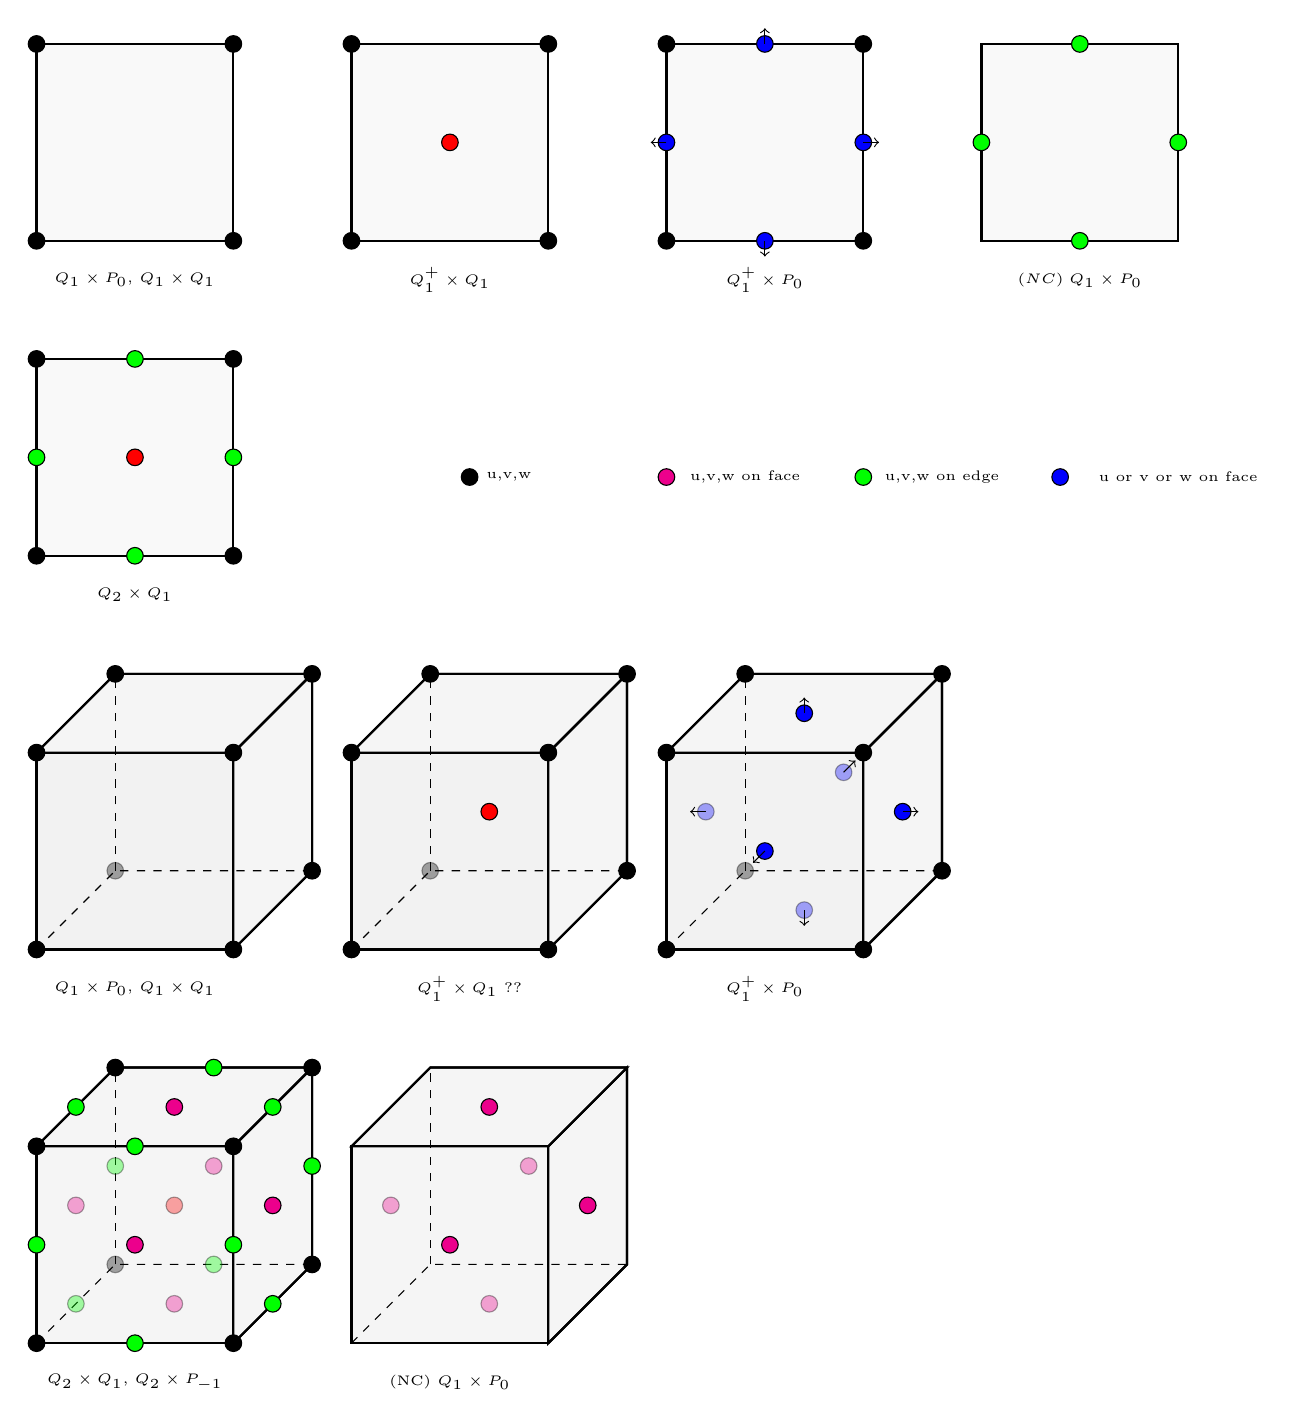
\begin{tikzpicture}
%\draw[fill=gray!23,gray!23](0,0) rectangle (20,10);
%\draw[step=0.5cm,gray,very thin] (0,0) grid (18,18); %background grid

%%%%%%%%%%%%%%%%%%%%%%%%%%%%%%%%%%%%%%%%%%%%%%%%%%%%%%%%%%%%%%%%%%%%
%bottom row
%%%%%%%%%%%%%%%%%%%%%%%%%%%%%%%%%%%%%%%%%%%%%%%%%%%%%%%%%%%%%%%%%%%%
\draw[thick,fill=gray!8] (1,1) -- (3.5,1) -- (3.5,3.5) -- (1,3.5) -- cycle;
\draw[thick,fill=gray!8] (5,1) -- (7.5,1) -- (7.5,3.5) -- (5,3.5) -- cycle;
%\draw[thick,fill=gray!8] (9,1) -- (11.5,1) -- (11.5,3.5) -- (9,3.5) -- cycle;
%\draw[thick,fill=gray!8] (13,1) -- (15.5,1) -- (15.5,3.5) -- (13,3.5) -- cycle;

%right sides
\draw[thick,fill=gray!8] (3.5,1) -- (4.5,2) -- (4.5,4.5) -- (3.5,3.5) -- cycle;
\draw[thick,fill=gray!8] (7.5,1) -- (8.5,2) -- (8.5,4.5) -- (7.5,3.5) -- cycle;
%\draw[thick,fill=gray!8] (11.5,1) -- (12.5,2) -- (12.5,4.5) -- (11.5,3.5) -- cycle;
%\draw[thick,fill=gray!8] (15.5,1) -- (16.5,2) -- (16.5,4.5) -- (15.5,3.5) -- cycle;

%tops
\draw[thick,fill=gray!8] (1,3.5) -- (3.5,3.5) -- (4.5,4.5) -- (2,4.5) -- cycle;
\draw[thick,fill=gray!8] (5,3.5) -- (7.5,3.5) -- (8.5,4.5) -- (6,4.5) -- cycle;
%\draw[thick,fill=gray!8] (9,3.5) -- (11.5,3.5) -- (12.5,4.5) -- (10,4.5) -- cycle;
%\draw[thick,fill=gray!8] (13,3.5) -- (15.5,3.5) -- (16.5,4.5) -- (14,4.5) -- cycle;

\draw[thick] (1,3.5) -- (2,4.5) -- (4.5,4.5) -- (4.5,2) -- (3.5,1);
\draw[thick] (5,3.5) -- (6,4.5) -- (8.5,4.5) -- (8.5,2) -- (7.5,1);
%\draw[thick] (9,3.5) -- (10,4.5) -- (12.5,4.5) -- (12.5,2) -- (11.5,1);
%\draw[thick] (13,3.5) -- (14,4.5) -- (16.5,4.5) -- (16.5,2) -- (15.5,1);

\draw[thick] (3.5,3.5) -- (4.5,4.5) ;
\draw[thick] (7.5,3.5) -- (8.5,4.5) ;
%\draw[thick] (11.5,3.5) -- (12.5,4.5) ;
%\draw[thick] (15.5,3.5) -- (16.5,4.5) ;

\draw[dashed] (1,1) -- (2,2) -- (4.5,2) ;\draw[dashed] (2,2) -- (2,4.5);
\draw[dashed] (5,1) -- (6,2) -- (8.5,2) ;\draw[dashed] (6,2) -- (6,4.5);
%\draw[dashed] (9,1) -- (10,2) -- (12.5,2) ;\draw[dashed] (10,2) -- (10,4.5);
%\draw[dashed] (13,1) -- (14,2) -- (16.5,2) ;\draw[dashed] (14,2)--(14,4.5);

\draw[black,fill=black] (1,1)   circle (3pt);
\draw[black,fill=black] (3.5,1)   circle (3pt);
\draw[black,fill=black] (3.5,3.5)   circle (3pt);
\draw[black,fill=black] (1,3.5)   circle (3pt);
\draw[black,fill=black] (2,4.5)   circle (3pt);
\draw[black,fill=black] (4.5,4.5)   circle (3pt);
\draw[black,fill=black] (4.5,2)   circle (3pt);
\draw[black,fill=black,opacity=0.35] (2,2)   circle (3pt);

%\draw[black,fill=black] (5,1)   circle (3pt);
%\draw[black,fill=black] (7.5,1)   circle (3pt);
%\draw[black,fill=black] (7.5,3.5)   circle (3pt);
%\draw[black,fill=black] (5,3.5)   circle (3pt);
%\draw[black,fill=black] (6,4.5)   circle (3pt);
%\draw[black,fill=black] (8.5,4.5)   circle (3pt);
%\draw[black,fill=black] (8.5,2)   circle (3pt);
%\draw[black,fill=black,opacity=0.35] (6,2)   circle (3pt);

%\draw[black,fill=black] (9,1)   circle (3pt);
%\draw[black,fill=black] (11.5,1)   circle (3pt);
%\draw[black,fill=black] (11.5,3.5)   circle (3pt);
%\draw[black,fill=black] (9,3.5)   circle (3pt);
%\draw[black,fill=black] (10,4.5)   circle (3pt);
%\draw[black,fill=black] (12.5,4.5)   circle (3pt);
%\draw[black,fill=black] (12.5,2)   circle (3pt);
%\draw[black,fill=black,opacity=0.35] (10,2)   circle (3pt);

%\draw[black,fill=black] (13,1)   circle (3pt);
%\draw[black,fill=black] (15.5,1)   circle (3pt);
%\draw[black,fill=black] (15.5,3.5)   circle (3pt);
%\draw[black,fill=black] (13,3.5)   circle (3pt);
%\draw[black,fill=black] (14,4.5)   circle (3pt);
%\draw[black,fill=black] (16.5,4.5)   circle (3pt);
%\draw[black,fill=black] (16.5,2)   circle (3pt);
%\draw[black,fill=black,opacity=0.35] (14,2)   circle (3pt);


%%%%%%%%%%%%%%%%%%%%%%%%%%%%%%%%%%%%%%%%%%%%%%%%%%%%%%%%%%%%%%%%%%%%
%3rd row 
%%%%%%%%%%%%%%%%%%%%%%%%%%%%%%%%%%%%%%%%%%%%%%%%%%%%%%%%%%%%%%%%%%%%

\draw[thick,fill=gray!5] (1,15) -- (3.5,15) -- (3.5,17.5) -- (1,17.5) -- cycle;
\draw[thick,fill=gray!5] (5,15) -- (7.5,15) -- (7.5,17.5) -- (5,17.5) -- cycle;
\draw[thick,fill=gray!5] (9,15) -- (11.5,15) -- (11.5,17.5) -- (9,17.5) -- cycle;
\draw[thick,fill=gray!5] (13,15) -- (15.5,15) -- (15.5,17.5) -- (13,17.5) -- cycle;

\draw[black,fill=black] (1,15)   circle (3pt);
\draw[black,fill=black] (3.5,15)   circle (3pt);
\draw[black,fill=black] (1,17.5)   circle (3pt);
\draw[black,fill=black] (3.5,17.5)   circle (3pt);
\node[] at (2.25,14.5) {\tiny $Q_1\times P_0$, $Q_1\times Q_1$};


\draw[black,fill=black] (5,15)   circle (3pt);
\draw[black,fill=black] (7.5,15)   circle (3pt);
\draw[black,fill=black] (5,17.5)   circle (3pt);
\draw[black,fill=black] (7.5,17.5)   circle (3pt);
\node[] at (6.25,14.5) {\tiny $Q_1^+\times Q_1$};
\draw[black,fill=red] (6.25,16.25)   circle (3pt);

\draw[black,fill=black] (9,15)   circle (3pt);
\draw[black,fill=black] (11.5,15)   circle (3pt);
\draw[black,fill=black] (9,17.5)   circle (3pt);
\draw[black,fill=black] (11.5,17.5)   circle (3pt);
\node[] at (10.25,14.5) {\tiny $Q_1^+\times P_0$};

\draw[black,fill=blue] (9,16.25)   circle (3pt);
\draw[black,fill=blue] (11.5,16.25)   circle (3pt);
\draw[black,fill=blue] (10.25,15)   circle (3pt);
\draw[black,fill=blue] (10.25,17.5)   circle (3pt);

\draw[fill=blue,->] (9,16.25) -- (8.8,16.25); 
\draw[fill=blue,->] (11.5,16.25) -- (11.7,16.25); 
\draw[fill=blue,->] (10.25,15) -- (10.25,14.8); 
\draw[fill=blue,->] (10.25,17.5) -- (10.25,17.7); 


\draw[black,fill=green] (14.25,15)   circle (3pt);
\draw[black,fill=green] (14.25,17.5)   circle (3pt);
\draw[black,fill=green] (13,16.25)   circle (3pt);
\draw[black,fill=green] (15.5,16.25)   circle (3pt);
\node[] at (14.25,14.5) {\tiny $(NC)\; Q_1\times P_0$};

%%%%%%%%%%%%%%%%%%%%%%%%%%%%%%%%%%%%%%%%%%%%%%%%%%%%%%%%%%%%%%%%%%%%
%2nd row 
%%%%%%%%%%%%%%%%%%%%%%%%%%%%%%%%%%%%%%%%%%%%%%%%%%%%%%%%%%%%%%%%%%%%

\draw[thick,fill=gray!5] (1,11) -- (3.5,11) -- (3.5,13.5) -- (1,13.5) -- cycle;
%\draw[thick,fill=gray!5] (5,11) -- (7.5,11) -- (7.5,13.5) -- (5,13.5) -- cycle;
%\draw[thick,fill=gray!5] (9,11) -- (11.5,11) -- (11.5,13.5) -- (9,13.5) -- cycle;
%\draw[thick,fill=gray!5] (13,11) -- (15.5,11) -- (15.5,13.5) -- (13,13.5) -- cycle;

\draw[black,fill=black] (1,11)   circle (3pt);
\draw[black,fill=green] (2.25,11)   circle (3pt);
\draw[black,fill=black] (3.5,11)   circle (3pt);
\draw[black,fill=green] (1,12.25)   circle (3pt);
\draw[black,fill=red] (2.25,12.25)   circle (3pt);
\draw[black,fill=green] (3.5,12.25)   circle (3pt);
\draw[black,fill=black] (1,13.5)   circle (3pt);
\draw[black,fill=green] (2.25,13.5)   circle (3pt);
\draw[black,fill=black] (3.5,13.5)   circle (3pt);
\node[] at (2.25,10.5) {\tiny $Q_2\times Q_1$};



%%%%%%%%%%%%%%%%%%%%%%%%%%%%%%%%%%%%%%%%%%%%%%%%%%%%%%%%%%%%%%%%%%%%
%1st row 
%%%%%%%%%%%%%%%%%%%%%%%%%%%%%%%%%%%%%%%%%%%%%%%%%%%%%%%%%%%%%%%%%%%%
\draw[thick,fill=gray!10] (1,6) -- (3.5,6) -- (3.5,8.5) -- (1,8.5) -- cycle;
\draw[thick,fill=gray!10] (5,6) -- (7.5,6) -- (7.5,8.5) -- (5,8.5) -- cycle;
\draw[thick,fill=gray!10] (9,6) -- (11.5,6) -- (11.5,8.5) -- (9,8.5) -- cycle;
%\draw[thick,fill=gray!10] (13,6) -- (15.5,6) -- (15.5,8.5) -- (13,8.5) -- cycle;

%right sides
\draw[thick,fill=gray!8] (3.5,6) -- (4.5,7) -- (4.5,9.5) -- (3.5,8.5) -- cycle;
\draw[thick,fill=gray!8] (7.5,6) -- (8.5,7) -- (8.5,9.5) -- (7.5,8.5) -- cycle;
\draw[thick,fill=gray!8] (11.5,6) -- (12.5,7) -- (12.5,9.5) -- (11.5,8.5) -- cycle;
%\draw[thick,fill=gray!8] (15.5,6) -- (16.5,7) -- (16.5,9.5) -- (15.5,8.5) -- cycle;

%tops
\draw[thick,fill=gray!8] (1,8.5) -- (3.5,8.5) -- (4.5,9.5) -- (2,9.5) -- cycle;
\draw[thick,fill=gray!8] (5,8.5) -- (7.5,8.5) -- (8.5,9.5) -- (6,9.5) -- cycle;
\draw[thick,fill=gray!8] (9,8.5) -- (11.5,8.5) -- (12.5,9.5) -- (10,9.5) -- cycle;
%\draw[thick,fill=gray!8] (13,8.5) -- (15.5,8.5) -- (16.5,9.5) -- (14,9.5) -- cycle;


\draw[thick] (1,8.5) -- (2,9.5) -- (4.5,9.5) -- (4.5,7) -- (3.5,6);
\draw[thick] (5,8.5) -- (6,9.5) -- (8.5,9.5) -- (8.5,7) -- (7.5,6);
\draw[thick] (9,8.5) -- (10,9.5) -- (12.5,9.5) -- (12.5,7) -- (11.5,6);
%\draw[thick] (13,8.5) -- (14,9.5) -- (16.5,9.5) -- (16.5,7) -- (15.5,6);

\draw[thick] (3.5,8.5) -- (4.5,9.5) ;
\draw[thick] (7.5,8.5) -- (8.5,9.5) ;
\draw[thick] (11.5,8.5) -- (12.5,9.5) ;
%\draw[thick] (15.5,8.5) -- (16.5,9.5) ;

\draw[dashed] (1,6) -- (2,7) -- (4.5,7)    ;\draw[dashed] (2,7) -- (2,9.5);
\draw[dashed] (5,6) -- (6,7) -- (8.5,7)    ;\draw[dashed] (6,7) -- (6,9.5);
\draw[dashed] (9,6) -- (10,7) -- (12.5,7)  ;\draw[dashed] (10,7) -- (10,9.5);
%\draw[dashed] (13,6) -- (14,7) -- (16.5,7) ;\draw[dashed] (14,7) -- (14,9.5);

\draw[black,fill=black] (1,6)   circle (3pt);
\draw[black,fill=black] (3.5,6)   circle (3pt);
\draw[black,fill=black] (3.5,8.5)   circle (3pt);
\draw[black,fill=black] (1,8.5)   circle (3pt);
\draw[black,fill=black] (2,9.5)   circle (3pt);
\draw[black,fill=black] (4.5,9.5)   circle (3pt);
\draw[black,fill=black] (4.5,7)   circle (3pt);
\draw[black,fill=black,opacity=0.35] (2,7)   circle (3pt);

\draw[black,fill=black] (5,6)   circle (3pt);
\draw[black,fill=black] (7.5,6)   circle (3pt);
\draw[black,fill=black] (7.5,8.5)   circle (3pt);
\draw[black,fill=black] (5,8.5)   circle (3pt);
\draw[black,fill=black] (6,9.5)   circle (3pt);
\draw[black,fill=black] (8.5,9.5)   circle (3pt);
\draw[black,fill=black] (8.5,7)   circle (3pt);
\draw[black,fill=black,opacity=0.35] (6,7)   circle (3pt);

\draw[black,fill=black] (9,6)   circle (3pt);
\draw[black,fill=black] (11.5,6)   circle (3pt);
\draw[black,fill=black] (11.5,8.5)   circle (3pt);
\draw[black,fill=black] (9,8.5)   circle (3pt);
\draw[black,fill=black] (10,9.5)   circle (3pt);
\draw[black,fill=black] (12.5,9.5)   circle (3pt);
\draw[black,fill=black] (12.5,7)   circle (3pt);
\draw[black,fill=black,opacity=0.35] (10,7)   circle (3pt);

%\draw[black,fill=black] (13,5)   circle (2pt);
%\draw[black,fill=black] (15.5,5)   circle (2pt);
%\draw[black,fill=black] (15.5,7.5)   circle (2pt);
%\draw[black,fill=black] (13,7.5)   circle (2pt);
%\draw[black,fill=black] (14,8.5)   circle (2pt);
%\draw[black,fill=black] (16.5,8.5)   circle (2pt);
%\draw[black,fill=black] (16.5,6)   circle (2pt);
%\draw[black,fill=black,opacity=0.35] (14,6)   circle (2pt);


\node[] at (2.25,5.5) {\tiny $Q_1\times P_0$, $Q_1\times Q_1$};


\node[] at (6.5,5.5) {\tiny $Q_1^+\times Q_1$ ??};
\draw[black,fill=red] (6.75,7.75)   circle (3pt);

\node[] at (10.25,5.5) {\tiny $Q_1^+\times P_0$};
\draw[black,fill=blue,opacity=0.35] (9.5,7.75)   circle (3pt);
\draw[black,fill=blue] (12,7.75)   circle (3pt);
\draw[black,fill=blue,opacity=0.35] (10.75,6.5)   circle (3pt);
\draw[black,fill=blue] (10.75,9)   circle (3pt);
\draw[black,fill=blue] (10.25,7.25)   circle (3pt);
\draw[black,fill=blue,opacity=0.35] (11.25,8.25)   circle (3pt);

\draw[fill=blue,->] (9.5,7.75) -- (9.3,7.75); 
\draw[fill=blue,->] (12,7.75) -- (12.2,7.75); 
\draw[fill=blue,->] (10.75,6.5) -- (10.75,6.3); 
\draw[fill=blue,->] (10.75,9) -- (10.75,9.2); 
\draw[fill=blue,->] (10.25,7.25)  -- (10.1,7.1) ;
\draw[fill=blue,->] (11.25,8.25)  -- (11.4,8.4) ;

\node[] at (2.25,0.5) {\tiny $Q_2\times Q_1$, $Q_2\times P_{-1}$};

\draw[black,fill=red,opacity=0.35] (2.75,2.75)   circle (3pt);

\draw[black,fill=magenta,opacity=0.35] (1.5,2.75)   circle (3pt);
\draw[black,fill=magenta] (4,2.75)   circle (3pt);
\draw[black,fill=magenta,opacity=0.35] (2.75,1.5)   circle (3pt);
\draw[black,fill=magenta] (2.75,4)   circle (3pt);
\draw[black,fill=magenta] (2.25,2.25)   circle (3pt);
\draw[black,fill=magenta,opacity=0.35] (3.25,3.25)   circle (3pt);

\draw[black,fill=green] (1,2.25)   circle (3pt);
\draw[black,fill=green] (3.5,2.25)   circle (3pt);
\draw[black,fill=green,opacity=0.35] (2,3.25)   circle (3pt);
\draw[black,fill=green] (4.5,3.25)   circle (3pt);
\draw[black,fill=green,opacity=0.35] (1.5,1.5)   circle (3pt);
\draw[black,fill=green] (4,1.5)   circle (3pt);
\draw[black,fill=green] (2.25,1)   circle (3pt);
\draw[black,fill=green,opacity=0.35] (3.25,2)   circle (3pt);
\draw[black,fill=green] (1.5,4)   circle (3pt);
\draw[black,fill=green] (4,4)   circle (3pt);
\draw[black,fill=green] (2.25,3.5)   circle (3pt);
\draw[black,fill=green] (3.25,4.5)   circle (3pt);

\node[] at (6.25,0.5) {\tiny (NC) $Q_1\times P_0$};
\draw[black,fill=magenta,opacity=0.35] (5.5,2.75)   circle (3pt);
\draw[black,fill=magenta] (8,2.75)   circle (3pt);
\draw[black,fill=magenta,opacity=0.35] (6.75,1.5)   circle (3pt);
\draw[black,fill=magenta] (6.75,4)   circle (3pt);
\draw[black,fill=magenta] (6.25,2.25)   circle (3pt);
\draw[black,fill=magenta,opacity=0.35] (7.25,3.25)   circle (3pt);

\draw[black,fill=black]   (6.5,12) circle (3pt); \node[] at (7,12) {\tiny u,v,w};
\draw[black,fill=magenta] (9,12) circle (3pt); \node[] at (10,12) {\tiny u,v,w on face};
\draw[black,fill=green] (11.5,12) circle (3pt); \node[] at (12.5,12) {\tiny u,v,w on edge};
\draw[black,fill=blue] (14,12) circle (3pt); \node[] at (15.5,12) {\tiny u or v or w on face};

%\draw[black,fill=blue] (1,3.5) circle (2pt); \node[] at (1,3.7) {\tiny \color{blue} 60};

%\draw[black,fill=green](14.75,4.75) circle (2pt);\node[] at (14.75,4.95){\tiny\color{green}121};

%\draw[black,fill=red] (6.25,4.75) circle (2pt); \node[] at (6.25,4.95) {\tiny \color{red} 148};

%\node[] at (1.5,2.75) {\tiny \color{magenta} (0)};


%\draw[thick,->] (0,3) -- (0,4); %x
%\draw[thick,->] (0,3) -- (1,2.5); %y
%\node[] at (1,2.125) {$y$};
%\node[] at (0.25,4) {$z$};

\end{tikzpicture}
\end{center}

Add DSSY, RT, Q1Q1+2 bubbles

\vspace{.5cm}

\begin{tabular}{llll}
\hline
2D &  \\ 
Rannacher-Turek & NCQ1P0 & \stone 77 & pb with buoyancy-driven flow \\
Lamichhane      & Q1+Q1  & \stone 72, \stone 74  & \\ 
DSSY            &        & \stone 77  pb with buoyancy-driven flow \\
Fortin          &        & \stone 80 \\
\hline
\hline
3D & \\
Rannacher-Turek & NCQ1P0  & \elefant &  \\
Lamichhane      & Q1+Q1   & \stone  & Does not work \\ 
DSSY & \\
Fortin & & \stone 81 \\
\hline
\end{tabular}
 %-------------------------------------
\newpage
\subsection{On the meaning of basis functions} \begin{flushright} {\tiny {\color{gray} basis\_functions\_meaning.tex.tex}} \end{flushright}
%~~~~~~~~~~~~~~~~~~~~~~~~~~~~~~~~~~~~~~~~~~~~~~~~~~~~~~~~~~~~~~~~~~~~~~~~~~~~~~~~~~~~~~~~~~~~~~~~~~


\subsubsection{In one dimension}

Let us consider a 1D domain subdivided in 3 elements. We then consider the four linear basis functions 
attached to each node. On the following sketch these are not depicted on a single element with 
reduced coordinates but instead for the whole domain in the natural coordinate $x$:



\begin{flushright} {\tiny {\color{gray} (tikz\_basisfunctions.tex)}} \end{flushright}
%~~~~~~~~~~~~~~~~~~~~~~~~~~~~~~~~~~~~~~~~~~~~~~~~~~~~~~~~~~~~~~~~~~~~~~~~~~~~~~~~~~~~~~~~~~~~~~~~~~

\begin{center}
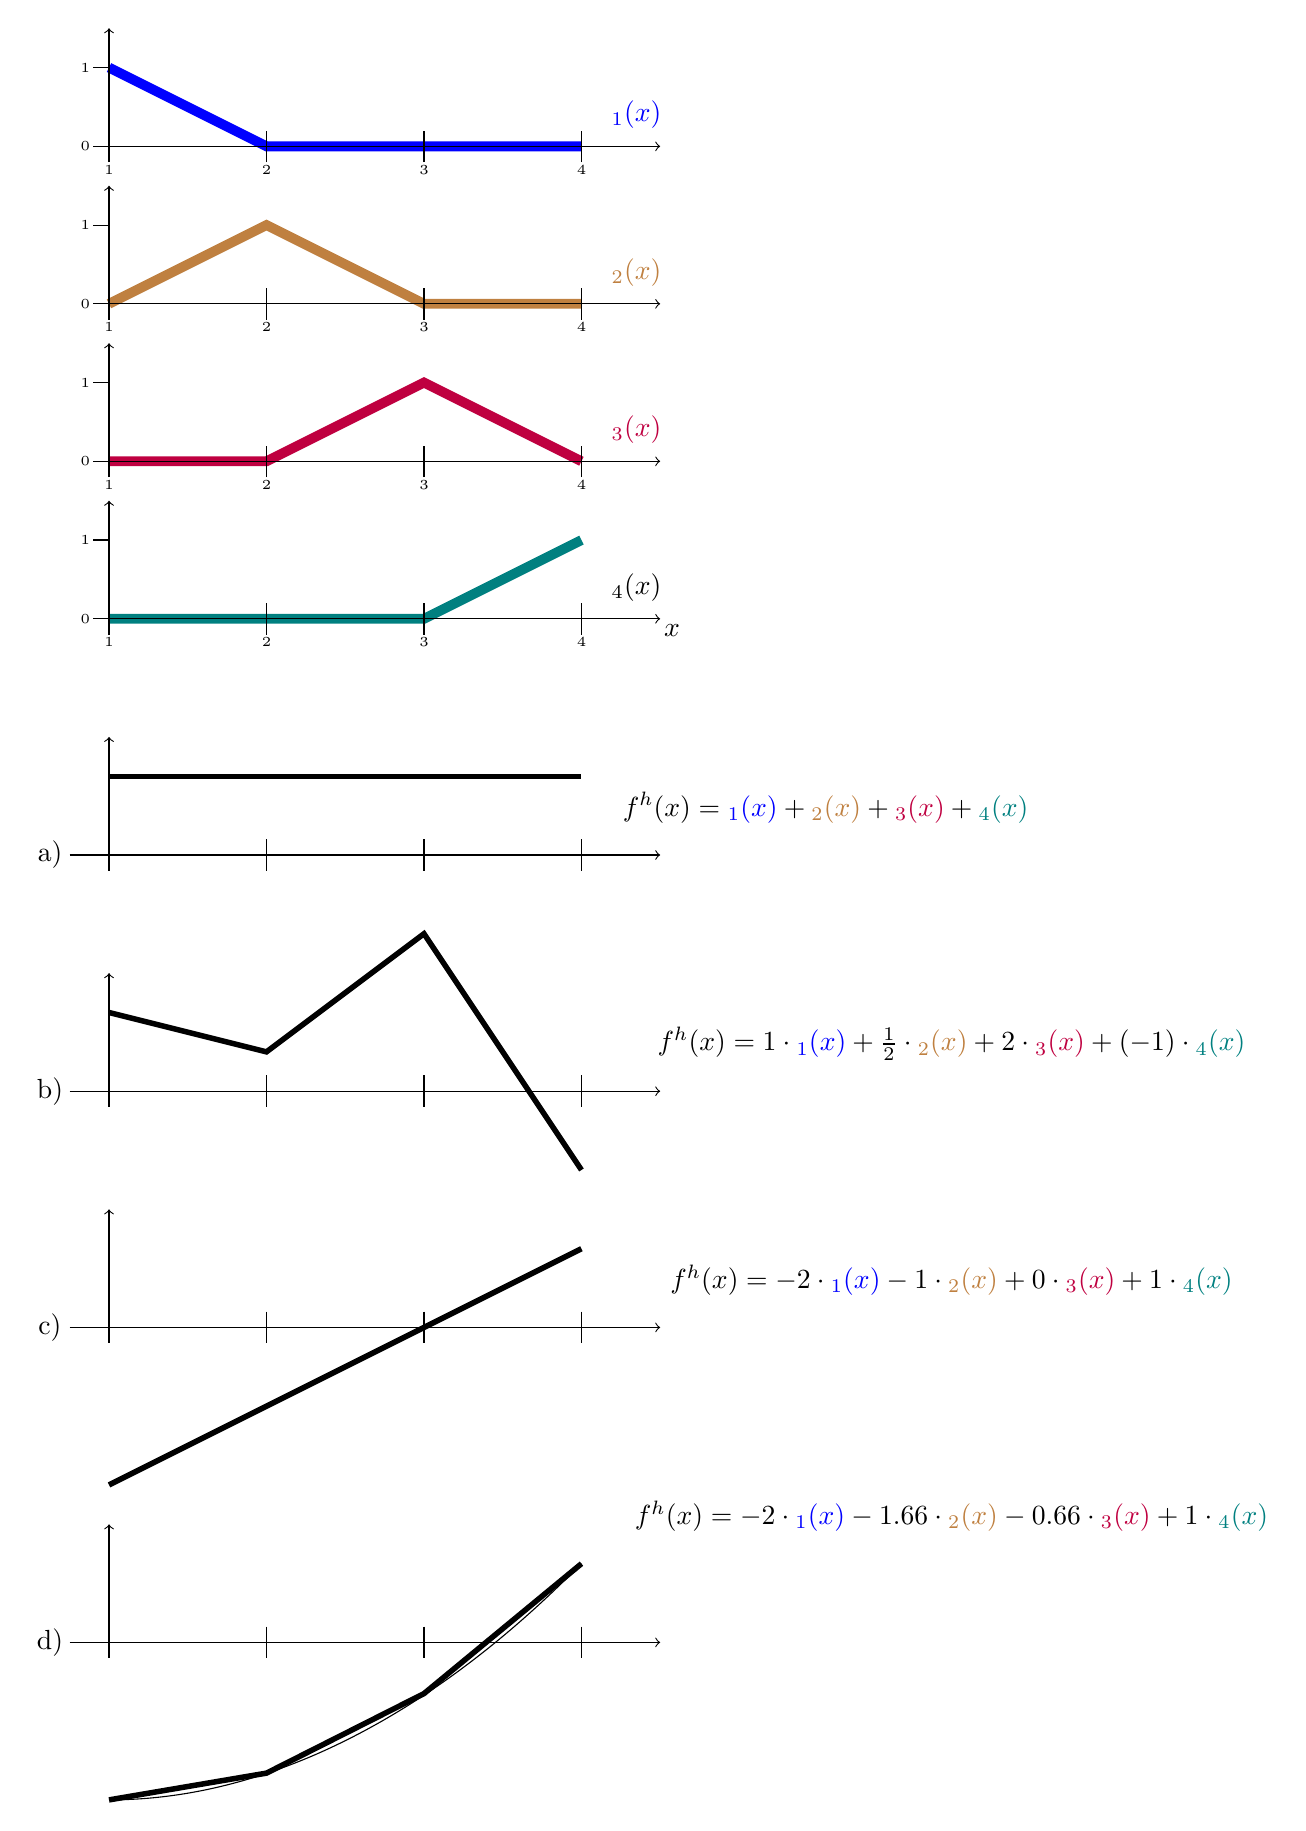
\begin{tikzpicture}
%\draw[step=0.5cm,gray,very thin] (0,-15) grid (15,10); 

%N1
\node[] at (7.7,7.4) {\color{blue}$\bN_1(x)$};
\draw[line width=1.25mm,color=blue] (1,8)--(3,7)--(5,7)--(7,7);
\draw [->] (0.8,7) -- (8,7);
\draw [->] (1,7) -- (1,8.5);
\draw [-] (1,6.8) -- (1,7.2);
\draw [-] (3,6.8) -- (3,7.2);
\draw [-] (5,6.8) -- (5,7.2);
\draw [-] (7,6.8) -- (7,7.2);

%N2
\node[] at (7.7,5.4) {\color{brown} $\bN_2(x)$};
\draw[line width=1.25mm,color=brown] (1,5)--(3,6)--(5,5)--(7,5);
\draw [->] (0.8,5) -- (8,5);
\draw [->] (1,5) -- (1,6.5);
\draw [-] (1,4.8) -- (1,5.2);
\draw [-] (3,4.8) -- (3,5.2);
\draw [-] (5,4.8) -- (5,5.2);
\draw [-] (7,4.8) -- (7,5.2);

%N3
\node[] at (7.7,3.4) {\color{purple}$\bN_3(x)$};
\draw[line width=1.25mm,color=purple] (1,3)--(3,3)--(5,4)--(7,3);
\draw [->] (0.8,3) -- (8,3);
\draw [->] (1,3) -- (1,4.5);
\draw [-] (1,2.8) -- (1,3.2);
\draw [-] (3,2.8) -- (3,3.2);
\draw [-] (5,2.8) -- (5,3.2);
\draw [-] (7,2.8) -- (7,3.2);

%N4
\node[] at (7.7,1.4) {$\bN_4(x)$};
\draw[line width=1.25mm,color=teal] (1,1)--(5,1)--(7,2);
\draw [->] (0.8,1) -- (8,1);
\draw [->] (1,1) -- (1,2.5);
\draw [-] (1,0.8) -- (1,1.2);
\draw [-] (3,0.8) -- (3,1.2);
\draw [-] (5,0.8) -- (5,1.2);
\draw [-] (7,0.8) -- (7,1.2);

\node[] at (8.15,0.85) {$x$};


\node[] at (1,6.7) {\tiny $1$};
\node[] at (3,6.7) {\tiny $2$};
\node[] at (5,6.7) {\tiny $3$};
\node[] at (7,6.7) {\tiny $4$};

\node[] at (1,4.7) {\tiny $1$};
\node[] at (3,4.7) {\tiny $2$};
\node[] at (5,4.7) {\tiny $3$};
\node[] at (7,4.7) {\tiny $4$};

\node[] at (1,2.7) {\tiny $1$};
\node[] at (3,2.7) {\tiny $2$};
\node[] at (5,2.7) {\tiny $3$};
\node[] at (7,2.7) {\tiny $4$};

\node[] at (1,0.7) {\tiny $1$};
\node[] at (3,0.7) {\tiny $2$};
\node[] at (5,0.7) {\tiny $3$};
\node[] at (7,0.7) {\tiny $4$};

\draw [-] (0.8,8) -- (1,8); \node[] at (0.7,7) {\tiny $0$}; \node[] at (0.7,8) {\tiny $1$};
\draw [-] (0.8,6) -- (1,6); \node[] at (0.7,5) {\tiny $0$}; \node[] at (0.7,6) {\tiny $1$};
\draw [-] (0.8,4) -- (1,4); \node[] at (0.7,3) {\tiny $0$}; \node[] at (0.7,4) {\tiny $1$};
\draw [-] (0.8,2) -- (1,2); \node[] at (0.7,1) {\tiny $0$}; \node[] at (0.7,2) {\tiny $1$};



\node[] at (0.25,-2) {a)};
\node[] at (10.1,-1.4) {$f^h(x)={\color{blue}\bN_1(x)}+{\color{brown} \bN_2(x)}
+{\color{purple}\bN_3(x)}+{\color{teal}\bN_4(x)}$};
\draw[line width=0.7mm] (1,-1)--(7,-1);
\draw [->] (0.5,-2) -- (8,-2);
\draw [->] (1,-2) -- (1,-0.5);
\draw [-] (1,-1.8) -- (1,-2.2);
\draw [-] (3,-1.8) -- (3,-2.2);
\draw [-] (5,-1.8) -- (5,-2.2);
\draw [-] (7,-1.8) -- (7,-2.2);

\node[] at (0.25,-5) {b)};
\node[] at (11.7,-4.4) {$f^h(x)=1\cdot {\color{blue}\bN_1(x)}+\frac12\cdot {\color{brown} \bN_2(x)}
+2\cdot {\color{purple}\bN_3(x)}+(-1)\cdot {\color{teal}\bN_4(x)}$};
\draw [->] (0.5,-5) -- (8,-5);
\draw [->] (1,-5) -- (1,-3.5);
\draw [-] (1,-4.8) -- (1,-5.2);
\draw [-] (3,-4.8) -- (3,-5.2);
\draw [-] (5,-4.8) -- (5,-5.2);
\draw [-] (7,-4.8) -- (7,-5.2);
\draw[line width=0.7mm] (1,-4)--(3,-4.5)--(5,-3)--(7,-6);

\node[] at (0.25,-8) {c)};
\node[] at (11.7,-7.4) {$f^h(x)=-2\cdot {\color{blue}\bN_1(x)}-1\cdot {\color{brown} \bN_2(x)}
+0\cdot {\color{purple}\bN_3(x)}+1\cdot {\color{teal}\bN_4(x)}$};
\draw [->] (0.5,-8) -- (8,-8);
\draw [->] (1,-8) -- (1,-6.5);
\draw [-] (1,-7.8) -- (1,-8.2);
\draw [-] (3,-7.8) -- (3,-8.2);
\draw [-] (5,-7.8) -- (5,-8.2);
\draw [-] (7,-7.8) -- (7,-8.2);
\draw[line width=0.7mm] (1,-10)--(3,-9)--(5,-8)--(7,-7);

\node[] at (0.25,-12) {d)};
\draw [->] (0.5,-12) -- (8,-12);
\draw [->] (1,-12) -- (1,-10.5);
\draw [-] (1,-11.8) -- (1,-12.2);
\draw [-] (3,-11.8) -- (3,-12.2);
\draw [-] (5,-11.8) -- (5,-12.2);
\draw [-] (7,-11.8) -- (7,-12.2);
\draw (1,-14) parabola (7,-11);
\draw[line width=0.7mm] (1,-14)--(3,-13.66)--(5,-12.65)--(7,-11);
\node[] at (11.7,-10.4) {$f^h(x)=-2\cdot {\color{blue}\bN_1(x)}-1.66\cdot {\color{brown} \bN_2(x)}
-0.66\cdot {\color{purple}\bN_3(x)}+1\cdot {\color{teal}\bN_4(x)}$};


\end{tikzpicture}
\end{center}





The four cases a,b,c,d are examples of combinations of these basis functions:
\[
f_h(x)=\sum_{i=1}^4 N_i(x) f_i
\]
Where $f_i$ are the values associated to the four nodes. 
We assume that the distance $h$ between nodes is 1.

Example a) illustrates the fact that the sum of all basis functions must be strictly equal to one everywhere
in the domain. Failing to do so would mean that the basis functions cannot represent a constant field (see
Section~\ref{ss:q12d}). 

Example b) illustrates a somewhat random combination of the basis functions, yielding a broken line. 

Example c) illustrates the fact that these linear basis functions can exactly represent a
linear function. When $f(x)=x-2$, then $f_1=f(0)=-2$, $f_2=f(1)=-1$, $f_3=f(2)=0$ and $f_4=f(3)=+1$, 
then $f_h(x)$ is exactly $f(x)$ on the domain.

Example d) illustrates the fact that linear basis functions cannot represent a parabola. Smaller and 
smaller elements will do an increasingly better job and will get closer to the curve but a 
systematic error will subsist.  


Note that these drawings are trivial to produce since $N_i(x_j)=\delta_{ij}$ by definition, so that 
$f_h(x_j)=f_j$.

%........................................................................
\subsubsection{In two dimensions}



 %-------------------
